\documentclass[11pt,partial,draft,doublespace]{aucklandthesis}
%
% This is a template for University of Auckland theses.
%
% Written by Alistair Kwan, June 2016
% 
%
% Options:
%	10pt, 11pt, 12pt: size of main text
% 	examcopy: asserts confidentiality for examination copies
%	partial: thesis partial fulfils degree requirements
%	singlespace, onehalfspace, doublespace: line spacing
%	oneside: format for single-sided printing
%	draft: adds 'draft' and date to footer
%

%%%% Packages introduced by me, not included with the template
\usepackage[normalem]{ulem}
\usepackage{amsmath}
\usepackage[binary-units]{siunitx}

%
% Add, delete or un-comment packages below as required.
%

\usepackage[utf8]{inputenc}
\usepackage[T1]{fontenc}

% Readability options
%
\usepackage{booktabs} % for table rules
\usepackage{microtype} % for improved justification

\usepackage{graphicx} % for inserting graphics files
\usepackage{appendix} % for appendices

% Typeface options — choose one if desired
% or choose a different typeface to accommmodate character sets
% as needed for East Asian and other languages.
%
% Consider compiling using the XeLaTeX engine if you have more extreme
% typeface needs, e.g. for multiple languages, or a need for symbols particular
% to a typeface.
%
% See also the LaTeX Symbols List at
% https://http://www.ctan.org/pkg/comprehensive
%
% \usepackage{mathptmx} % Times New Roman, including mathematics
% \usepackage{mathpazo} % Palatino with mathematics support
% \usepackage{fourier} % Utopia, a serif typeface with Fourier mathematics
% \usepackage{gentium} % a contemporary serif typeface
% \usepackage{libertine} % a softer-feeling serif typeface; also installs sans-serif font Biolinum
% \usepackage{fouriernc} % Century Schoolbook with Fourier maths
% \usepackage{mathpple} % Palatino with Fourier maths


% To set the sans serif font (for \sffamily):
%\usepackage[scaled]{helvet} % Nimbus, like Helvetica
%\usepackage{universalis} % Universalis
%\usepackage{avant} % URW Gothic, like Avant Garde
%\usepackage{PTSansNarrow}
%\usepackage{AlegreyaSans} % Alegreya Sans

% To set the mathematics font:
%\usepackage{eulervm} % Euler, based on a Zapf design

% To set the (usually monospaced) typewriter font:
%\usepackage[ttdefault=true]{AnonymousPro}
%\usepackage[scaled]{beramono}
%\usepackage{inconsolata}
%\usepackage{sourcecodepro}

%\usepackage{cjk} % for Chinese, Japanese, Korean

\usepackage{tabularx} % For easier table formatting.

% \usepackage[nottoc]{tocbibind} % Controls the table of contents
%   nottoc: don't list table of contents inside itself
%   section: go as far as section-level headings

% Automated bibliography
%
\usepackage[
	style=numeric-comp, 
% 	citestyle=authortitle,
	backend=biber,
	sorting=nyt,
	sortcites=true,
	]
	{biblatex}
	\addbibresource{bib/stereo.bib}
	\addbibresource{bib/compmodels.bib}
	\addbibresource{bib/psystems.bib}
	\addbibresource{bib/languages.bib}
% bibliography{bibliography1.bib, bibliography2.bib} % Specify bibliography files 
% bibliography{bib/stereo.bib, Mendeley.bib}

% The below was copied verbatim from https://tex.stackexchange.com/a/154875 on 9 December 2019, and then modified to reverse the ordering of the URL and DOI fields.  The purpose of it is to suppress the use of the URL field if the DOI field is defined - thus avoiding the many instances where the URL is printed, but is just a link to the DOI (besides which, in the PDF the DOI becomes a link to the DOI site).  It seems to work for my purposes.
\DeclareSourcemap{
  \maps[datatype=bibtex]{
    \map{
      \step[fieldsource=doi,final]
      \step[fieldset=url,null]
    }  
  }
}

\usepackage{hyperref} % for formatting web addresses and other URLs
\urlstyle{same} % try also tt, sf if this option doesn't produce clear enough output

%%% All the glossaries stuff was put here, since the Glossaries documentation says it should be used after hyperref.

\usepackage[acronym,noredefwarn,toc]{glossaries}
\setacronymstyle{long-short}
\makeglossaries

% The below was taken from https://tex.stackexchange.com/a/562932.  It is used in the glossary.tex file, but placed here because I'm not sure putting it in the glossary file won't b0rk things.  It was originally called 'newdefineabbreviation', but I changed it because that was irritatingly long.
% #1 - reference e.g. api
% #2 - Short e.g. API
% #3 - Full name e.g. Application Programming Interface
% #4 - Description
\newcommand{\newdefacr}[4]
{
    % Glossary entry
    \newglossaryentry{#1-glossary}
    {
        text={#2},
        long={#3},
        name={\glsentrylong{#1-glossary} (\glsentrytext{#1-glossary})},
        description={#4}
    }

    % Acronym
    \newglossaryentry{#1}
    {
        type=\acronymtype,
        name={\glsentrytext{#1-glossary}}, % Short
        description={\glsentrylong{#1-glossary}}, % Full name
        first={\glsentryname{#1-glossary}\glsadd{#1-glossary}},
        see=[Glossary:]{#1-glossary} % Reference to corresponding glossary entry
    }
}

\loadglsentries{glossary}

\begin{document}

% \newcommand{\cml}{Concurrent~ML}
% \newcommand{\csp}{Communicating Sequential Processes}
\newcommand{\fsharp}{F\nolinebreak\hspace{-.05em}\raisebox{.3ex}{\tiny{\textbf{\#}}}}
\newcommand{\cps}{cP~systems}

% ====================================================
%
% FRONTMATTER
%
% Arabic pagination, starting with the title page
% which is counted but not numbered
%
% ====================================================

% Specify the title page content
\title{Message Passing-Based Stereo Matching Algorithms in cP~systems and Concurrent~ML}
%\subtitle{Using functional programming to make life simpler and promote efficiency}
\author{James Cooper}
\degreesought{Doctor of Philosophy} 
\degreediscipline{Computer Science}
\degreecompletionyear{2021}

% Print the title page
\maketitle

% Abstract, up to 350 words
\begin{abstract}
    
% \Gls{mc}, also known as \gls{ps}, is a field of theoretical computer science initially inspired by the principles of the interactions of chemicals within, and their movements through, the membranes of biological cells.  An important property of most types of \gls{ps} is that they are inherently concurrent, with the contents of every membrane evolving simultaneously, and that they have an unbounded space capacity, empowering them to solve traditional computationally challenging problems quickly.  \gls{cps} is a type of \gls{ps} that takes a high-level approach to modelling problems in \gls{mc}, allowing for more straightforward solutions while retaining the advantages for time complexity.

\Gls{mc}, also known as \gls{ps}, is a field of theoretical computer science initially inspired by the principles of the interactions of chemicals within, and their movements through, the membranes of biological cells.  Important properties of most types of \gls{ps} are that they
\begin{inparaenum}[a)]
\item are inherently concurrent, with the contents of every membrane evolving simultaneously; and,
\item that they have an unbounded space capacity, empowering them to solve traditional computationally challenging problems quickly.
\end{inparaenum}
\gls{cps} is a type of \gls{ps} that takes a high-level approach to modelling problems in \gls{mc}, allowing for more straightforward solutions while retaining the advantages for time complexity.
    
This dissertation applies \gls{cps}' capacity for large-scale concurrency to established problems in computer science, including the \glsentrylong{tsp-glossary}, the \glsentrylong{gcp-glossary}, and image \gls{medianfilter}ing.  It also explores from a new angle the pre-existing concept termed here ``\glsxtrlong{nmp}'', which involves separate logical \glsxtrlongpl{pe} communicating with their neighbours via messaging.  A critical difference, explored in some depth in this dissertation, between \glsxtrlong{nmp} and similar concepts is the requirement for a \glsxtrlong{pe} to compute outgoing messages to neighbours based on the messages received from every neighbour \emph{except} the intended recipient.
    
Novel \gls{cps} solutions to the \glsentrylong{tsp-glossary} and \glsentrylong{gcp-glossary}, with time complexity linear to the number of nodes in the graph, along with a constant-time solution to median filtering, are presented.  Experiments with computer implementations of solutions validate those solutions and explore the efficacy of different implementation methods.

Three variants of \glsxtrlong{nmp} are also explored.  Firstly, the traditional \gls{gs} style used in \glsxtrlong{bp}, then an asynchronous approach which is closer to the underlying concept but seemingly so far unexplored, and finally an intermediate \gls{ls} form that naturally arises from studying the previous two.  Analysis of and experiments with these variants show that the \gls{gs} and \gls{ls} styles compute identical results, but the \gls{ls} one is approximately 5-13\% faster in general practice, while the asynchronous variant is typically around another 10\% faster again yet computes almost-identical results.
    
\end{abstract}
 % it's in a separate file

% Dedication (optional)
%\thesisdedication{Dedicated to grandma, and to grammar.}
% \thesisdedication{This work is dedicated to the interested reader and all those who make use of material presented within.}

% Preface and/or acknowledgements (optional)
% \chapter*{Preface}

Significant parts of this dissertation are based on papers published previously.  In particular: \Cref{chap:tsp}, \nameref{chap:tsp}, is based on \cite{Cooper2019}.  \Cref{chap:gcol}, \nameref{chap:gcol}, is based on \cite{Cooper2019a}.  \Cref{chap:median}, \nameref{chap:median}, presents work from \cite{Cooper2018} and \cite{Cooper2021}.  \Cref{chap:nmp}, \nameref{chap:nmp}, presents work which appeared in an early form in \cite{Cooper2020}, and which has been significantly revised and is under review with the Journal of Membrane Computing as at the time of submission of this dissertation.

\section*{Acknowledgements}

Acknowledgement must be made, firstly, of my supervisors, Doctor Radu Nicolescu and Associate Professor Patrice Delmas.  Without their support and guidance, I certainly would have never made it to this point.  So too must acknowledgement be made of Professor Emeritus Georgy Gimel'farb and Doctor Wannes van der Mark, both of whom have provided invaluable support at times.%  The two Heads of School during my time as a PhD candidate, Professor Robert Amor and Associate Professor Giovanni Russello, have also been supportive of me in their own ways.

Furthermore, thanks must be given to the professional staff from: the School of Computer Science; the School of Graduate Studies; Libraries and Learning Services (particularly those who served as Computer Science subject librarian); the Centre for eResearch; and the wider University of Auckland.  Particular mention must be made of Kaleigh Fennah, Emma Gavenda, Sue Skelly, Sarah Sneyd and Robyn Young.

I also would like to mention several people who were students contemporaneously with me (and in a few cases were also co-authors with me), including: Arabella Anderson; Mihailo Azhar; Daniel Britten; Doctor Trevor Gee; Alec Henderson; Yan Kolezhitskiy; Yezhou Liu; William Hsu; and Eirian Perkins.  Each of these people in some way has improved my time and experience during the PhD process.

I'm fairly sure there are further people who should be mentioned, but I'm afraid that I can't recall them specifically at the time of writing.

% Everyone who assisted me with the use of the languages in [choiceoflang chapter], especially those people who responded to my requests for assistance on the MLton and Guile mailing lists, and in the Racket Slack workspace.  Special mention must be made of: Yawar Raza from the Rochester Institute of Technology, who routinely answered my questions about MLton very quickly and helpfully; and [soegaard2 from Racket slack]

Lastly, and above all else, mention must be made of my mum.  Thanks mum!

\vspace{1cm}
\hfill James Cooper

\hfill Auckland, New Zealand

\hfill September 2021

 % it's in a separate file

% Contents, lists of tables and figures
\settocdepth{subsection} % choose chapter, section, subsection 
\cleardoublepage\tableofcontents
%\cleardoublepage\listoffigures
%\cleardoublepage\listoftables

% Glossary (optional)
% % \makeglossaries

% Acronyms (sorted in alphabetical order by their label, rather than their full definition)

%% A-M
\newacronym{bp}{BP}{belief~propagation}
\newacronym{cp}{CP}{concurrent~propagation}
\newacronym{csp}{CSP}{communicating sequential processes}
\newacronym{dpsm}{DPSM}{dynamic~programming \gls{sm}}
\newacronym{dsp}{DSP}{digital signal processor}
\newacronym{enps}{ENPS}{enzymatic numerical P~systems}
\newacronym{fifo}{FIFO}{first-in-first-out}
\newacronym{fpga}{FPGA}{field-programmable gate array}
\newacronym{fps}{FPS}{frames per second}
\newacronym{gpu}{GPU}{graphics processing unit}
\newacronym{gpgpu}{GPGPU}{general-purpose \glsxtrshort{gpu}}
\newacronym{lbp}{LBP}{loopy belief~propagation}
\newacronym{mpbsm}{MPBSM}{message passing-based \gls{sm}}
% \newacronym{mpi}{MPI}{Message Passing Interface}
\newacronym{mrf}{MRF}{Markov random field}
\newacronym{mwt}{MWT}{moving window transform}

%% N-Z
\newacronym{ndcsm}{NDCSM}{noise-driven concurrent \gls{sm}}
\newacronym{nm}{NM}{neighbourhood messaging}
\newacronym{nmp}{NMP}{neighbourhood message passing}
\newacronym{oq}{OQ}{oracle query}
\newacronym{pe}{proxel}{processing element}
\newacronym{pram}{PRAM}{parallel random access machine}
\newacronym{sad}{SAD}{sum of absolute differences}
\newacronym{skps}{SKPS}{simple kernel P~systems}
\newacronym{ssd}{SSD}{sum of squared differences}

% Combo glossary & acronyms

% A-M
\newdefacr{blas}{BLAS}{basic linear algebra subprograms}{Basic Linear Algebra Subprograms}{A collection of low-level functions, typically written in Fortran, to perform core linear algebra processes such as vector and matrix addition and multiplication.  The netlib implementation of BLAS is considered the ``reference'' implementation (see \url{https://www.netlib.org/blas/}), but other implementations are available --- in particular, some hardware vendors may produce their own version optimised for their particular hardware, such as Nvidia's cuBLAS.  Many, perhaps most, high-performance mathematical libraries in higher-level programming languages, \eg{} Python's Numpy, make use of a BLAS implementation internally.}
\newdefacr{cml}{CML}{Concurrent~ML}{Concurrent~ML}{A programming style introduced by John Reppy as an extension of the pre-existing programming language Standard~ML;  specifically, the Standard~ML of New Jersey implementation.  Conceptually, Concurrent~ML has a lot in common with \glsxtrlong{csp}.  Both involve each logical process mostly advancing on its own, but sometimes synchronising with others over channels (see also \vref{fig:back:cml_exchange}).  Concurrent~ML is described in detail in \cite{Reppy2007}.}
\newdefacr{gcp}{GCP}{graph colouring problem}{Graph Colouring Problem}{The problem of finding a way to colour the nodes in a graph, such that no adjacent nodes share a colour.  This problem is typically further constrained to using a maximum number of colours for the entire graph, or finding the minimum number of colours required to perform the colouring.}
\newdefacr{hcp}{HCP}{Hamiltonian cycle problem}{Hamiltonian Cycle Problem}{Closely related to the \glsdesc{hpp}.  In this problem, the Hamiltonian Path must also be a cycle, \ie{} it ends back at the origin node.}
\newdefacr{hpp}{HPP}{Hamiltonian path problem}{Hamiltonian Path Problem}{The problem of determining whether, for a given graph, there exists a traversal of the graph in which each node is visited exactly once.}
\newdefacr{lapack}{LAPACK}{linear algebra package}{Linear Algebra Package}{A (relatively) low-level software library for performing more advanced linear algebra processes, such as solving systems of linear equations, or matrix factorizations \eg{} LU, QR and Cholesky Decompositions.  LAPACK is typically built atop \glstext{blas}, meaning that it is highly portable and efficient across different hardware architectures, so long as a good quality \glstext{blas} implementation is available.  There reference implementation of LAPACK can be found at \url{https://www.netlib.org/lapack/} but others are available too.}
\newdefacr{lhs}{LHS}{left-hand side}{Left-hand Side}{A part of the definition of a \gls{cps} rule.  It is the list of terms which \emph{must} be present and as-yet unused in a rule at the current step, in order for the current rule to be applicable.  All terms appearing here are deleted from the containing cell at the end of the step.}

% N - Z
\newdefacr{rhs}{RHS}{right-hand side}{Right-hand Side}{A part of the definition of a \gls{cps} rule.  It is the list of terms which are created by the rule's application, and appear in the relevant cell at the end of the step.}
%
% \newdefacr{sgm}{SGM}{semi-global~matching}{Semi-global~Matching}{Semi-global~matching is a \gls{sm} algorithm introduced by Hirschmüller that, as the name suggests, sits somewhere between traditional global and local \gls{sm} algorithms.  This provides advantages in that retains much of the speed advantage of local algorithms, while also receiving much of the benefit derived from taking into consideration a larger part of the total input images.}
%
\newdefacr{tsp}{TSP}{travelling salesman problem}{Travelling Salesman Problem}{An extension of the \glsdesc{hcp}.  Here, the edges between nodes have weights, and the goal of the problem is to find a minimum weight Hamiltonian cycle on the graph.}

% Glossary Entries
% \newglossaryentry{}{name={},description={}}

%% A-M
\newglossaryentry{actor}{text={actor},name={Actor},description={A model of message-passing-based concurrent programming originally developed  chiefly by Carl Hewitt.  Its defining characteristics are that it uses asynchronous messaging, whereby the sender and receiver do not need to coordinate or synchronise at all; and that instead of using channels or similar as a go-between, Actors send messages directly to each other, which necessitates ``knowing'' (\ie{} holding a reference to) the intended recipient.  Notable examples of implementations of Actors are found in the programming languages Erlang and Pony, and the Scala library Akka.}}
%
\newglossaryentry{clps}{text={cell-like P~systems},name={Cell-like P~Systems},plural={cell-like P~system},description={The original \gls{ps} variant first proposed by Gheorghe Păun, based on the operation of chemicals inside biological cells.  The main characteristic of cell-like P~systems is that the chemicals are represented by a potentially-infinite variety of atomic objects, and are contained within one or more membranes.  Every cell-like P~system has an outermost membrane, the \emph{skin membrane} which separates the cell from the \emph{environment}, and may have more membranes inside itself.  These latter membranes are nested in such a fashion that they resemble a graphical tree.  Each membrane has a separate \gls{ruleset}, though the \glspl{ruleset} are not necessarily unique.  Rules may create and remove chemicals based on the presence (or absence) or other chemicals inside a membrane, and also send chemicals to an inner \emph{child} membrane, or to an outer \emph{parent} membrane.  Perhaps due to it being the original variant (and thus pre-dating the term ``cell-like P systems''), some forms of P~systems which could be regarded as cell-like are not necessarily labelled as such, \eg{} P~systems with active membranes.}}
%
\newglossaryentry{compartment}{text={compartment},name={Compartment},description={A generic umbrella term for the processing units, which also act as the containers of the system's objects, of a given \gls{ps} type.  For example, these are: the membranes of \gls{clps}; the cells of \gls{tlps}; the neurons of \gls{snps}; and the \glspl{tlc} of \gls{cps} --- though in the case of \gls{cps} the data-only complex objects are sometimes also described as sub-compartments or micro-compartments, because they still contain objects.}}
%
\newglossaryentry{cps}{text={cP~systems},name={cP~Systems},description={A variant of \gls{ps} created by Radu Nicolescu.  The main point of difference between cP~systems and other variants is that, in general, cP~systems is `higher-level'.  That is, instead of specifying (semi-)uniform families of rules customised to each specific problem of a given type, cP~systems \glspl{ruleset} typically cover all possible problem specifications without customisation ahead-of-time through the use of variables.  The cP~systems `runtime' performs unification over the variables.  Furthermore, only the \glspl{tlc} have associated rules, and all other terms contained within are merely inert objects.  See also \cref{chap:cpsystems}.},plural={cP~system}}
%
\newglossaryentry{disparity}{text={disparity},name={Disparity},description={The shift, measured as a number of pixels, of a point in one stereo image to its location in the other image.  When combined with information about the cameras used to capture the images which is derived from calibration, the measured disparity is used to estimate the distance from the cameras to the point in the scene.  Disparity is often also referred to as `parallax'.}}
%
\newglossaryentry{disparitymap}{text={disparity map},name={Disparity Map},description={An output array/image (often just using a single channel of 8- or 16-bit integers) which encodes the final estimated disparities for every pixel in the input images.  The range of values in a disparity map itself is restricted to range of possible disparities used in the \gls{sm} algorithm.  It is common, however, to adjust the disparity map in some fashion to make differences in disparity estimates more visible through techniques such as histogram equalisation.  Most published figures of disparity maps will have had such an adjustment applied to make them more useful.  Disparity maps are sometimes also referred to as `digital parallax maps.'}}
%
\newglossaryentry{fne}{description={The `standard' neighbourhood arrangement in situations such as \glsxtrlong{bp}.  When used in reference to a grid, it typically means the other locations in the grid immediately to the left, right, above and below.},text={four-neighbourhood},name={Four-neighbourhood}}
%
\newglossaryentry{functor}{description={In the context of \gls{cps}, a functor is the label applied to the delimiters of a complex term.  \Eg{} for \(\cpfunc{a}{\cpfunc{b}{c}}\) both \(a\) and \(b\) are functors, because they are the outer label for their respective inner terms.  ``Functor'' is also sometimes used as a shorthand to refer to the complex term as whole.  Strictly speaking, this is incorrect, but used for convenience nevertheless, as writing \enquote{the complex term denoted by the functor \(a\)} is usually overly verbose.},text={functor},name={Functor}}
%
\newglossaryentry{gs}{description={In the context of \glsxtrlong{nmp}, this refers to an approach to messaging whereby the entire lattice waits until every \glsxtrshort{pe} in the lattice has finished its messaging for a given generation before proceeding to the next generation.},text={globally-synchronous},name={Globally-synchronous}}
%
\newglossaryentry{inhibitor}{name={Inhibitor},text={inhibitor},description={In \gls{cps}, an inhibitor on a rule denotes an object which \emph{must not} be present in the relevant \gls{tlc} for the rule to be applicable.}}
%
\newglossaryentry{ls}{description={In the context of \glsxtrlong{nmp}, this refers to an approach to messaging whereby every \glsxtrshort{pe} in the lattice waits until it has received \emph{all} messages pertaining to one generation before accepting any messages pertaining to a subsequent generation.},text={locally-synchronous},name={Locally-synchronous}}
%
\newglossaryentry{mc}{text={membrane computing},name={Membrane Computing},description={A computational model inspired by the functioning of biological systems, specifically the interactions of chemicals inside the membranes of a biological cell.  The terms Membrane Computing and P systems are normally used interchangeably.}}
%
\newglossaryentry{mecosim}{name={MeCoSim},description={Software used to simulate arbitrary P~systems, from a multitude of variants.  MeCoSim was created and is maintained by researchers from Universidad de Sevilla (University of Seville) in Spain (see further \cite{MeCoSim}).  Generally, rules for a given system are specified with a \gls{plingua} file.  These rules can then be run on a specific set of starting objects, with MeCoSim reporting the outcome from executing the rules at the end of each step.}}
%
\newglossaryentry{medianfilter}{text={median filter},name={Median Filter},description={An image processing technique often used to remove `salt \& pepper' noise from images.  Every pixel's value is updated to the median value of it and its neighbours, in a given neighbourhood.  It is an embarassingly-parallel problem in that each pixel in the image can compute its median without relying on other pixels' results, so long as it can observe their current value.  The necessity for performing selection, however, means that it is non-trivial to implement a fast median filter.  It does not easily reduce to basic arithmetic operations only.}}
%
\newglossaryentry{ms}{text={micro-surgery},name={Micro-surgery},description={An alternative operation that can be performed on \gls{cps}' compound terms.  Instead of each rule application seizing control of the entire term, it merely takes hold of a subset of the terms contents.  A major benefit of this is to enable in a single step arithmetic on numeric multisets that would instead require iterations to complete.},plural={micro-surgeries}}

%% N-Z
\newglossaryentry{promoter}{name={Promoter},text={promoter},description={In \gls{cps}, a promoter on a rule denotes an object which \emph{must} be present in the relevant \gls{tlc} for the rule to be applicable, but which is \emph{not} consumed or deleted by the rule.}}
%
\newglossaryentry{ps}{name={P~Systems},see={mc},text={P~systems},description={An alternative name for \gls{mc}.},plural={P~system},}
%
\newglossaryentry{plingua}{name={P-Lingua}, description={A plain-text markup language used to represent \gls{ps} specifications in computer files, readable by both humans and computers.}}
%
\newglossaryentry{ruleset}{text={ruleset},name={Ruleset},description={The rules associated with a particular \gls{compartment} in a given \gls{ps} variant.}}
\newglossaryentry{sm}{text={stereo~matching},name={Stereo~Matching},description={A family of methods to match points from different images of the same scene to estimate the distance from the capturing cameras to objects in the scene.}}
\newglossaryentry{snps}{text={spiking neural P~systems},name={Spiking Neural P~Systems},description={Spiking neural P~systems is one of the three main \gls{ps} variants in common use today, and was introduced most recently.  Whereas \gls{clps} is based on intra-cellular chemical interactions, and \gls{tlps} on inter-cellular interactions, spiking neural P~systems is explicitly based on the idea of neurons in the brain interacting via synapses.  In principle, the communication-based nature of spiking neural P~systems makes it closer to \gls{tlps} than \gls{clps}, but unlike those two it uses only a single object in its alphabet, the spike.  This difference can make solutions to some problems more complex, but has the advantage that it makes it (comparatively) easy to implement those solutions with linear algebra operations.}}
\newglossaryentry{tlc}{text={top-level cell},name={Top-level Cell},description={The processing units of \gls{cps}, loosely equivalent to the skin membrane of other P~systems variants.  These are the only objects in the system which have rules and are `active'.  Generally, all other objects present in a system except channels are found inside a top-level cell.}}
\newglossaryentry{tlps}{text={tissue-like P~systems},name={Tissue-like P~Systems},description={Tissue-like P~systems is one of the oldest \gls{ps} variants, especially of those still in common use, and is based on the transmission of chemicals between cells via channels in biological tissue (rather than movement of chemicals through membranes within a cell like \gls{clps}).  A notable aspect of tissue-like P~systems is that they often include no ability for the cells to process their own contents.  Instead, all computation arises as a consequence of the communication.},plural={tissue-like P~system}}

% ====================================================
%
% MAINMATTER
%
% Include external chapter files here using
% the \input{} command
%
% If you run out of memory during compilation,
% switch some or all chapters to \include{} instead of \input{}, 
% but watch out for pagination problems.
%
% ====================================================

\chapter{Introduction}
Some wordiness will go here.

\section{My first section}
Post-introductory wordiness

\begin{anfxerror}{Describe development?}
    There have been a few twists \& turns before settling on the final dissertation topic, but some of the earlier work very much has had a significant impact on the getting to the final topic.  How much of that should be discussed in the intro, even though it isn't actually directly relevant to the current topic?
\end{anfxerror}

% Main goal:  To achieve at least one of the below
% \begin{itemize}
% \item run more efficiently (faster and/or use less memory)
% \item Scalability.  If one only scales well up to, say 4-8 cores, but the other works up to a much larger number of cores, then that would suggest that the latter approach is much more future-proof, since best guesses still suggest that manycore systems are the way of the future.
% \item `cleaner'/nicer code (by some reasonably objective, quantifiable measure)
% \item `easier to program/easier to read' -- lower complexity (how does one measure that though?)
% \end{itemize}

% Why is message passing better than using an algorithmic skeleton?  Or how much can the two ideas be unified?  (e.g. a \gls{cml} inspired skeleton for operations on regular grids -- perhaps using specific neighbourhoods).

\Gls{bp} can be described in terms of message passing, but also can be given fairly efficient \gls{gpu} implementations.  How do the two connect?

\begin{anfxwarning}{What goes in the intro?}
From \url{https://abacus.bates.edu/~ganderso/biology/resources/writing/HTWsections.html}:  ``the Introduction must answer the questions, "What was I studying? Why was it an important question? What did we know about it before I did this study? How will this study advance our knowledge?"''
\end{anfxwarning}

\section{Research Questions}
\begin{enumerate}
    % \item Can real-time message passing-based stereo matching be implemented using a message passing programming approach?
    % \item How do the results compare with more traditional implementations?
    % \item 
    \item Does modelling \gls{nmp} in a theoretical setting like \gls{cps} help in some way?
    \item Does an asynchronous model of \gls{nmp} reveal any benefit over the traditional synchronous versions?
    \item Does the practical implementation of \gls{nmp}, applied to \gls{bp} for \gls{sm} show any improvement over other techniques?
\end{enumerate}

\subsection{Research Question One}
% Here real-time means achieving a speed of at least 1 frame per second, i.e. at least 1 Hz.

\subsection{Research Question Two}
% Comparisons can be (will be?) made based on runtime efficiency, both with `wall time' taken and peak memory use, as well as based on code-quality measures in some fashion.  Also, if possible, check how well each approach scales.

\subsection{Research Question Three}

\section{Hypotheses}

\subsection{Hypothesis One}
% On larger/more powerful systems, yes.  On smaller systems (e.g. Nvidia Jetson Nano) no.

\subsection{Hypothesis Two}
% \gls{mpbsm} will be \emph{slower} than traditional methods, and use more memory.  The program will be longer, but it will be more clearly logically structured.  It will scale better than traditional approaches though, when there is shared memory but distinct processors.

\subsection{Hypothesis Three}

\section{Outline}
Where I summarise the upcoming dissertation (this section probably needs a different/better name).  Where in the intro do I explain the novelty?
\chapter{Background and Related Work}
\fxerror{Some of this probably should be chopped now...}{This review of related past work} focuses on the three main areas of Computer Science that are relevant to this dissertation:  Stereo Matching, Formal Models of Computation (especially \gls{ps}), and \glsentrylong{cml-glossary}.  In none of these cases does the review come close to comprehensively covering the entire span of the given area.  It merely tries to cover as much of the relevant recent and classic work as possible, while giving an extremely brief introduction to these areas.  The interested reader who is unfamiliar with any of these topics is strongly advised to refer to the materials cited.

% See \url{http://forneylab.org/} for something seemingly quite similar to what I'm doing...;  fglib \url{https://github.com/danbar/fglib};  IGraph library \url{https://igraph.org/};  LGNpy \url{https://github.com/ostwalprasad/LGNpy};  

\section{Formal Models of Concurrent Computation}
Perhaps the earliest (or at least, the earliest that is still widely known) formalised model of concurrent computation is the Petri Net \cite{Dennis2011}, first conceived of by Carl Petri, initially for the purpose of describing chemical processes \cite{Petri2008}.

\begin{anfxerror}{Why not Petri Nets?}
Why are Petri Nets not more popular?  Why do we choose \gls{csp} or \glspl{actor} or \gls{ps} over them?
\end{anfxerror}

\cite{Varela2013}

This work 

\subsection{\glsentrylong{csp} \& Pi~Calculus}
\gls{csp} is a `process algebra' and abstract model of concurrent computation put forward by Hoare \cite{Hoare1985,Roscoe2011}.  A typical sequential computation is represented by a `process'.  Processes' ``behaviour is described in terms of the occurrence and availability of abstract entities called \textit{events}'' \cite[p.~478]{Roscoe2011}.  Should more than one event be available simultaneously for a given process, then one will be chosen non-deterministically.  This choice is internal to the process, and not influenced by or visible to any other process.  %E.g. for a situation where there is one possible event \(a\) at a given point in time, the process \(P\) will choose that event and then proceed according to the result, written as: \[ a \rightarrow P(a) \]

Concurrency is introduced by the existence of multiple processes.  In general, the processes evolve independently, responding to events as they come.  Should a particular event appear in the alphabet of multiple processes, however, then all processes \emph{must} choose to participate in that event at the same time.  Should all processes involved make such a choice, they engage in a synchronous multi-way atomic synchronisation (hence `communicating').  \gls{csp} has provided significant inspiration for concurrency design in a number of programming languages, notably including Ada \cite{Defense1983,Taft2013}, Occam \cite{Elizabeth1987}, Google's Go \cite{Meyerson2014} (not to be confused with the earlier language Go! \cite{Clark2004}, which itself was explicitly designed for concurrency) and \gls{cml} \cite{Reppy2011}. 

Milner appreciated \gls{csp}, which advanced concurrency models by explicitly incorporating \emph{synchronised} interaction, something Milner's earlier Calculus for Communicating Systems \cite{Milner1980} had lacked  \cite{Milner1993}.  Milner still regarded \gls{csp} as incomplete, however, in that it had no support for the concept of `mobility' -- i.e. the ability of the system to reconfigure itself during operation.  Pi Calculus was created as an attempt to build upon those earlier systems but present a complete calculus of concurrent computation in much the same way that Lambda Calculus \cite{Barendregt1984} is a complete calculus for sequential computation.\footnote{Milner also pointed out that sequential computation is, in fact, a special case of concurrent computation.}

\subsection{\label{subsec:actors}\texorpdfstring{\Glspl{actor}}{Actors}}
The \gls{actor} \cite{Agha1986} model was introduced by Hewitt \cite{Hewitt1973}.  Much like \gls{csp} \& its cousins, the \gls{actor} model is based around the concept of separated, sequential but communicating processes which exchange messages.  Again, the processes make decisions and proceed based on their communications.  A key difference, however, is that in the \gls{actor} model the message exchanges are \emph{a}synchronous.  Each \gls{actor} has its own `mailbox', and may send messages to other \glspl{actor} so long as it knows their name (which is equivalent for this purpose to a concept of an address for the \gls{actor}), \emph{but does not wait at all for a response before proceeding}.

The \gls{actor} model is a popular one for concurrent programming, possibly owing to its intuitive concept.  The fact that communication is asynchronous makes \glspl{actor} much more suitable for modelling distributed systems without shared memory than \gls{csp} or similar -- \glspl{actor} can send messages and proceed without (necessarily) needing to wait for a response, instead continuing to process based on the messages they themselves have received.  By contrast, a system with synchronous communication would have prohibitive time costs, given the relative slow speed of typical links between distributed computers as compared to their capacity for local processing.  Many \gls{actor} systems have been implemented for different programming languages (e.g. \cite{Varela2001,Srinivasan2008,Charousset2016,Bernstein2016} \fxnote[inline,nomargin]{[need more refs?]}), and in fact it is a core component, and perhaps largely responsible for the success, of Erlang/OTP \cite{Armstrong2010,Armstrong2013,Vinoski2012}.  A relatively new language, Pony \cite{Clebsch2015,Clebsch2017}, takes this even further.
\begin{anfxnote}{Positive example for actors?}
In Concurrency in .NET, Terrell described using an actor to control access to a shared resource and stated that it was an extremely effective solution.
\end{anfxnote}

\Glspl{actor}, when used for non-trivial real-world software, have been criticised at times \cite{Welsh2013,Stucchio2013}.  While some of the criticisms described are implementation-specific (relating to Akka, a Scala \gls{actor} library), a common thread is that \glspl{actor} do not compose well.  This has the negative consequence that it is difficult to combine an \gls{actor} with anything else to create a new abstraction, and can require extensive modifications in source code to make relatively simple changes.

\subsection{Join Calculus}

\begin{anfxwarning}{Join Calc refs}
Chemical abstract machine, joinads, Scala communicating objects (IIRC, that was join calculus based), reagents
\end{anfxwarning}

\subsection{Others}
Mobility calculus.  Others?

% \subsection{Criticisms}

% Gorlatch \cite{Gorlatch2004} argued against basic message passing, decrying it as an unnecessary and unhelpful complication and favouring \fxerror*{What does `collective operations' mean?}{`collective' operations} instead.  This criticism focused upon \gls{mpi} as it was at the time, however, and made no reference to either Actors or \gls{csp}. \fxerror{Does subsection this truly belong here?}

\section{\glsentrytext{ps}/\glsentrytext{mc}}
\gls{ps}, also known as \gls{mc} (the two terms are generally used interchangeably), is a bio-inspired model of computing created by Păun in the late 1990s \cite{tPaun98a,Paun2000}, originally conceived of by considering the process of chemical reactions and exchanges that occur inside living biological cells \& the membranes within, and regarding this process as a form of computation.

Păun describes \gls{mc} \cite[p.~VII]{Paun2002} as:
\begin{quote}
Membrane computing is a branch of natural computing which abstracts from
the structure and the functioning of living cells. In the basic model, the membrane
systems - also called P systems - are distributed parallel computing
devices, processing multisets of objects, synchronously, in the compartments
delimited by a membrane structure. The objects, which correspond to chemicals
evolving in the compartments of a cell, can also pass through membranes.
The membranes form a hierarchical structure - they can be dissolved, divided,
created, and their permeability can be modified. A sequence of transitions between
configurations of a system forms a computation. The result of a halting
computation is the number of objects present at the end of the computation
in a specified membrane, called the output membrane. The objects can also
have a structure of their own that can be described by strings over a given
alphabet of basic molecules - then the result of a computation is a set of
strings.
\end{quote}

\Gls{mc} works analogously to a typical modern electronic computer, in that the system stores data, and processes \& updates those data based on a predefined program, with a view to arriving at a computable answer based on the starting state and any inputs to the system \cite{Paun2002,Paun2010b}.  In the case of \gls{ps}, the data are multisets of symbols, representing various chemicals and their quantities.  These are found inside one or more cells, based on real biological cells, which (to a certain extent at least) form a hybrid between main memory and the processing units of a computer.  The instructions of the program itself are provided by rules, which specify transformations of objects and interactions with the surrounding environment and other membranes or cells.

There are now, broadly, three main families of \gls{ps} variants:  \gls{clps} \cite{Paun2001,Paun2002}, \gls{tlps} \cite{tMaPaPaRo01a,Martin-Vide2003} and \gls{snps} \cite{Ionescu2006}.\footnote{Several other variants have been created, but most are used infrequently, if ever.  Apart from Numerical \gls{ps} and \gls{cps}, described in \autoref{subsec:numpsys} and \autoref{subsec:cpsys} respectively, this work will not address them.}  \Gls{clps} is the original, and sees objects compartmented into `membranes', which are arranged in a graphical tree structure with the outermost membrane (separating the cell from its environment) as the root of the tree.  In most variants, objects can evolve inside a membrane, but also be communicated between membranes (and the environment).  Furthermore, membranes can divide or dissolve themselves, and may have one or more special properties, such as `polarization' \cite{Paun1999a}.

Conversely, \gls{tlps} and \gls{snps} both arrange their computing compartments, named `cells' or `neurons' respectively, as nodes in arbitrary digraphs, with the edges between them representing connecting channels.  Whereas \gls{clps} emphasise the evolution of multisets of objects inside compartments, \gls{tlps} and \gls{snps} emphasise communication between separate cells/neurons, and many \gls{tlps} variants do not include any capacity for internal evolution inside cells -- if new objects are required, they are imported via communication with the environment, which is considered to possess an unlimited number of all objects, but has no rules of its own.

While \gls{tlps} have arbitrary alphabets, only one object is used in \gls{snps}, the `spike'.  This means that \gls{tlps} are frequently much like \gls{clps} in that they have custom objects for each purpose, with the key difference (usually) being in how the \glspl{prox} are arranged relative to each other and the choice between the two motivated primarily by which one seems like a better fit to the computation to be modelled.

Conversely, \gls{snps} represent everything through the use of differing quantities of the spike, kept in different neurons.  This means that it can be more complex to model certain problems, but also arguably means that \gls{snps} are, \textit{prima facie}, closer to Lambda Calculus \cite{Barendregt1984} and Church Numerals \fxerror[inline]{[ref]}, as well as Register Machines \fxerror[inline]{[ref]} (and indeed Register Machines have been simulated with \gls{snps} \fxerror[inline]{[ref]}).  All three approaches have been proven Turing-universal though \fxerror[inline]{[ref]}, so all three should be capable of expressing the same computations in different forms.  Furthermore, because \gls{snps} can easily be represented numerically, they lend themselves well to vector/matrix representations \cite{Zeng2010}.  This means that, potentially, \gls{snps} implementations can take advantage of high-performance techniques such as using \gls{blas} and/or \glspl{gpu} \cite{Aboy2019}.

Arguably, the most notable and important aspects of \gls{ps} models are that they:  i) Generally have no space limit.  That is, they contain an arbitrary number of cells, objects and membranes;  ii) Across all cells and membranes, all rules that can be applied are applied, as many times as possible given the current number of objects available.  These two features mean that \gls{ps} have unbounded space and processing capacity, which can be used to solve traditionally computationally-difficult problems relatively quickly \cite{Sosik2003,Jimenez2003,Paun1999a,Henderson2020}.  Most of these solutions, however, rely on trading time complexity for space complexity.  While this works in the theoretical framework, electronic simulations of the systems do not have access to unlimited instantaneous memory space, meaning many of the fast solutions are impractical with current real-world computers, e.g. \cite{Cooper2019} \fxnote[inline]{[refs]}.

\Gls{mc} is not just a theoretical model with limited practical use, however.  Besides Image Processing \& Computer Vision (see \autoref{subsec:imgprocpsys}), \gls{ps} variants have been applied to a range of fields, from power grid management to robotic control systems \cite{Zhang2017}.  [P-Lingua and simulation systems, e.g. MeCoSim]

\subsection{\label{subsec:numpsys}Numerical \glsentrytext{ps}}
Numerical P systemsss

\subsection{\label{subsec:cpsys}\glsentrytext{cps}}
\cite{Nicolescu2014b,Nicolescu2017}

\gls{cps} is another variant of \gls{ps}, developed by Nicolescu and collaborators in the early 2010s \fxerror[inline]{[ref]}.  It is largely based on \gls{clps}, and can be seen, to some extent at least, as a higher-level abstraction over it \cite{Nicolescu2018}.  It can also incorporate elements of \gls{tlps}, however, in that it includes concepts of channels and message passing between cells \cite{Henderson2019}.  Nicolescu, Ipate \& Wu demonstrated that not only is \gls{cps} capable of performing the same tasks as other \gls{ps} variants, but also can be used fairly cleanly to model typical computer programs \cite{Nicolescu2014a}.

The major advantage of \gls{cps} over traditional \gls{clps} is a simplification in the specification of complete systems to solve a given problem.  \gls{clps} (as well as \gls{tlps} and \gls{snps}) typically require the definition of a family of rulesets customised to the specific instance of the problem at hand, whereas \gls{cps} usually requires only the definition of a fixed (usually much shorter) set of rules that cover all possible instances.  Only inputs to the system need vary to solve different instances of the problem, e.g. in \cite{Cooper2019} only five fixed rules were needed to solve any instance of the Travelling Salesman Problem, with only customisation of the input objects (in this case, elements describing the nodes and edges of the graph) required.



\subsection{\label{subsec:imgprocpsys}Image Processing and Computer Vision in P~systems}
\cite{Zhang2012}

Perhaps owing to the unbounded potential space and parallelism of \gls{ps}, combined with the embarrassingly parallel nature of many tasks in Image Processing \& Computer Vision, the latter has proved to be fertile ground for the former, although not every publication puts its model to the test with a computerised simulation, or if it does, the authors may only provide scant details \cite{Diaz-Pernil2019}.  

Christinal, Díaz-Pernil \& Real \cite{Christinal2011} described a family of \gls{tlps} to perform region-based segmentation of both 2D and 3D images.  Despite their family of systems requiring only two cells, it also needed custom rule sets based on the size of the images as well as the number of colours present, with a number of rules per set proportional to the same measurements.  The paper showed the results of simulating the system, but provides no details on performance.

Díaz-Pernil \textit{et al.} \cite{Diaz-Pernil2013} commented that ``... commonly [a] parallel algorithm needs to be re-designed with only slight references to the [sequential original].  ... the design of a new parallel implementation not inspired by the sequential one allows ... the proposal of new creative solutions.''  They then demonstrated this fact by designing a new edge detection and segmentation algorithm named `A Graphical P (AGP) segmentator', inspired by the Sobel operator (see e.g. \cite{Nixon2012}) and using the segmentation method from \cite{Christinal2011}, which they modelled in \gls{tlps}.  The authors implemented their new algorithm on a \gls{gpu} and compared it with an implementation of the 3x3 and 5x5 Sobel operators, finding that theirs had near-identical runtimes but superior edge detection capabilities.

Díaz-Pernil \textit{et al.} \cite{Diaz-Pernil2013a} further explored modelling classic image processing techniques by implementing Guo \& Hall's binary image skeletonisation technique \cite{Guo1989} with \gls{snps}.  The overall system's rules templates are reasonably simple, but include references to a set \(DEL\) (used as a lookup to determine whether a cell should turn white or stay black) which does not appear to be modelled inside the system, meaning that it is not self-contained.  The authors simulated this system on a \gls{gpu}, but found that their implementation was upwards of twice as slow as another pre-existing implementation.  Confusingly, however, they state that one of the reasons for this is ``that the use of an alphabet with only one object, the spike \(a\), does not fit in the GPU architecture''.  This statement is difficult to understand, given that spikes can easily be represented as simple integers.  The authors also commented that the synchronous nature of the model is unrealistic, and imposing a global clock upon the system can be problematic.

Nicolescu \cite{Nicolescu2014} alternatively applied \gls{cps} to image skeletonisation based on Guo \& Hall's technique \cite{Guo1989}, presenting three forms of a solution: Synchronous versions that use multiple or a single cell (essentially the latter replicates the former via the use of sub-membranes), and an asynchronous multi-cell version.  The asynchronous version no longer assumes that all messages are passed between cells simultaneously and instantaneously, compensating for this by increasing the number of messages used.  This form, while arguably more realistic to modern computers, requires a greater message complexity. A prospective \gls{actor}-model-based (see \autoref{subsec:actors}) simplified implementation using \fsharp{}'s \texttt{MailboxProcessor} \cite[ch.~11]{Syme2015a} was presented also, but no results from running it were reported.

Nicolescu \cite{Nicolescu2015a} further applied \gls{cps} to seeded region growing of grayscale images.  The described system used a two-level approach, based on the `Structured Grid Dwarf' of the 13 Berkeley Dwarves \cite{Asanovic2006}, where the image was divided into rectangular blocks of multiple pixels.  Each block was modelled with a single cell, inter-block processing was carried out via message passing, and intra-block processing was performed by typical object evolution.  It was again suggested that this would fit well to the \gls{actor} model.

Díaz-Pernil \textit{et al.} \cite{Diaz-Pernil2016} built upon their AGP segmentator algorithm to create a version that works with RGB images rather than grayscale and applied it to a common medical Computer Vision task, isolating the `optic disc' in images of the inner eye.  With this they used the skeletonisation algorithm from \cite{Diaz-Pernil2013a} and a number of other steps not based on \gls{ps} to produce a complete imaging pipeline.  The authors implemented this on a \gls{gpu}, and found that their system was both more accurate and faster than previous systems.

Most directly relevant to the current work are \cite{GimelFarb2013a,Gimelfarb2011,Nicolescu2014b}, which model Dynamic Programming \gls{sm} in \gls{ps}, and indeed saw the genesis of \gls{cp} (\autoref{subsec:concprop}).  

\subsubsection{\glsentrytext{ps} on \glsentrylongpl{gpu}}
In many instances, a \gls{ps} model for a problem involves many separate small elements processing their data separately, and perhaps updating each other's state at the end of a step.  Given that this sounds remarkably close to the Single-Instruction Multiple-Thread \cite[Ch. 4.4.1]{Hennessy2012} nature of modern \gls{gpgpu}, it is no surprise that there has been much work put into simulating \gls{ps} on \glspl{gpu}.

\cite{Cecilia2010,Cecilia2010a,Cecilia2013,Macias-Ramos2015,Martinez-Del-Amor2015,Martinez-Del-Amor2013a,Maroosi2014,Maroosi2014a}


% \section{\glsentrylong{mpbsm}}

% \subsection{Preliminaries}
% What do I actually need to put in here?

% \subsubsection{Stereo Matching}

\subsection{\label{subsec:smgeneral}\glsentrytext{sm} in General}
Szeliski defines \gls{sm} \cite[p. 469]{Szeliski2011} as ``the process of taking two or more images and estimating a 3D model of the scene by finding matching pixels in the images and converting their 2D positions into 3D depths.''  It is essentially an attempt to replicate one of the techniques the brain uses to provide depth perception,\footnote{The brain has others, such as exploiting familiarity with everyday objects to estimate their actual size, and thus their rough distance from the eyes.} namely correlating the images received from each eye to estimate the distances to objects within view, but using digital images and a computer.

Indeed, \gls{sm} is not the only method for computer depth perception in use \cite{Sinha2020}.  Other approaches include, for example, Structured Light \cite{Giancola2018}, Time-of-Flight \cite{Hansard2013} and LiDAR \cite{Dong2017}.  \Gls{sm} has some advantages over those other techniques, though.  It is the only one which is entirely passive, i.e. it takes in data from the environment without interacting with it in some way, whereas the other three all involve projecting some form of light into the environment.  It is also arguably quicker to perform the necessary observations of the environment than the other methods, in that only a single pair of images need be captured, which can be accomplished in the time it takes for the pixel values to be read from the sensor planes into storage.  The choice of which method is most appropriate depends heavily upon the intended use of the computerised depth perception.  Or, if sufficient processing power is available, two or more of them can be used in combination to offset each other's weaknesses \cite{Zanuttigh2016}.

The `canonical' stereo camera arrangement is two cameras arranged in parallel, with a small horizontal offset between them.  This configuration leads to a general expectation that changes in the points in the scene will be shifted along one image's x-axis as compared to the other image's.  The identified distance of a shift is termed the `\gls{disparity}', and is used with other information about the cameras to compute an estimate to the matched points in the scene.  Generally, it is \fxnote*{name of assumption?}{assumed} that points in the image from the left camera will appear further to the right in said image as compared the same point in the right camera's image, and vice versa.

\begin{figure}
    \centering
    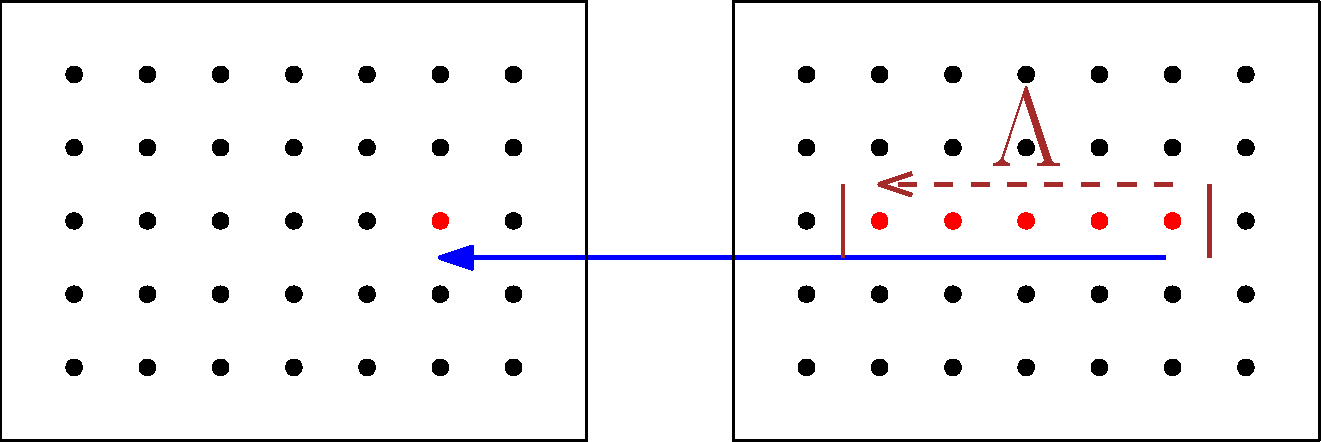
\includegraphics[width=1.0\textwidth]{chapters/litreview/images/stereo_matching-eps-converted-to.pdf}
    \caption{Diagram of the basic process of \gls{sm}. In this instance, for each pixel in the left image, a horizontal range of the pixels in the right image are searched, to find the one on the right that matches most closely to the one on the left. This has the effect that the \gls{disparitymap} is from the perspective of the left camera. The red dots represent the compared pixels. The brown dashed arrow and vertical bars represent the range of pixels in the right image to compute matching scores against. The length of the range is the lesser of the number of pixels before reaching the left border of the image, or the maximum \gls{disparity}, which is a parameter set by the user and represented here by \(\Lambda\).  Image from \cite{bsmpcvpic}.}
    \label{fig:stereomatchingbasic}
\end{figure}

% While precise approaches vary, the vast majority of \gls{sm} algorithms utilise some form of pixelwise comparison between images.  The basic process for this is shown in \autoref{fig:stereomatchingbasic}.    This comparison function be as simple as taking the absolute difference of the pixels under comparison.

In the general case \gls{sm} is impossible to perform perfectly because it is an ill-posed problem \cite{Gimelfarb1998}.  Going from a three-dimensional scene to a two-dimensional image necessarily involves a loss of information.  For any given image there are potentially an unbounded number of possible real-world scenes that could produce said image.  Using multiple images -- the more the better -- for \gls{sm} permits some recovery of information, but the process inevitably suffers from various sources of noise (where `noise' is defined broadly).

Liu \textit{et al.} \cite{Liu2005} describe four types of noise:  Signal, geometric, electronic and optical.  Signal noise arises from the normal operation of digital cameras, and electronic from differences between the internal operation of cameras used to capture images from different perspectives of the same scene.  Optical noise mainly stems from differences in the intensity and colour of light seen by the cameras at different perspectives when capturing images of the scene, caused by differences in the interactions between the objects of the scene and the available light sources at different points.  Lastly, geometric noise is a natural consequence of the fact that different perspectives must be used, and can be caused by issues as simple as the fact that points visible in one scene may not be visible in the other -- so-called `occlusions', caused by one part of the scene obscuring another part.

A key consequence of the last source of noise is the fact that, even in ideal circumstances with multiple `perfect' cameras, flawless lighting throughout the scene and \fxnote*{Provide reference for Lambertian surfaces}{objects which do not reflect light differently at different parts of their surfaces}, occlusions mean that for an arbitrary scene it is impossible to be certain a given algorithm has achieved a perfect reconstruction of the depths of the scene \cite{Gimelfarb1998}.  Strictly speaking, it \emph{is} possible that \gls{sm} produces an entirely accurate \gls{disparitymap}, but there would be no way to know without the use of additional information.

\fxwarning[inline,nomargin]{Include some example images to show the idea of stereo matching?}

\subsubsection{Image Rectification}
To reduce the computational complexity involved in performing \gls{sm}, many, perhaps most, algorithms only directly compare pixels along a single line in each image, typically the same horizontal line \cite[Ch. 11]{Szeliski2011}.  If the lines in the two images do not correspond to roughly the same part of the scene, then the matching process will likely fare poorly.  Such a discordance can occur when the cameras were not adequately aligned in terms of their spatial positions and angles relative to each other at the time of mutual image capture.

To overcome the challenges caused by mismatched lines, stereo image pairs are usually `rectified' (see e.g. \cite[Ch. 1.5.1]{Wohler2013}), wherein the captured images are adjusted so that they were effectively \fxerror*{Rectification could be described more precisely}{taken by properly aligned cameras}.  If rectification is performed well, the lines in the image should be properly aligned.  The parameters used in rectification in turn are deduced via camera calibration (see e.g. \cite[Ch. 1.4]{Wohler2013}), though neither topic is discussed further here.  For current purposes, all stereo image sets used are assumed to have been appropriately rectified already.

\begin{anfxnote}{}
    Discuss epipolar geometry?
\end{anfxnote}

\subsubsection{Middlebury}
\fxnote[inline,nomargin]{Talk about the Middlebury benchmarks, resources and website here.}

\subsubsection{Local vs Global}
\fxerror*{Expand/explain}{\cite{Scharstein2002}  (similar terms were in use earlier \cite{Gimelfarb1998})}

Perhaps the simplest and most obvious ways to perform \gls{sm} involve simply comparing the values of pixels in one image to the values of pixels in the other.

\subsubsection{\glsentrylong{mrf} \& Bayesian Inference}
\fxerror*{Expand/explain}{\cite{Kolmogorov2015,Blake2011}}

Not all global \gls{sm} algorithms utilise message passing, e.g. Graph Cuts \cite{Kolmogorov2001,Tappen2003}

Geman \& Geman \cite{Geman1984} showed that \glspl{mrf} are equivalent to Gibbs Distributions and that the two could be applied usefully to image tasks \cite{Gimelfarb1999}.

\begin{anfxwarning}{Pixel similarity measures}
    Move the below discussion about pixel similarity measures further up, probably into the \gls{sm} in general section?
\end{anfxwarning}

Frequently, in global methods the function used for the data cost is quite simplistic.  Most common is the use of simple absolute difference between the intensities of the pixels compared.  Other popular methods include \gls{sad} and \gls{ssd} \fxerror[inline]{[ref]}, adaptive window methods \cite{Yoon2005,Yoon2006}, and Birchfield \& Tomasi's Pixel Dissimilarity Measure \cite{Birchfield1998}.

In general, most \gls{mrf} approaches to \gls{sm} tend to use a truncated linear function to estimate the discontinuity/smoothness cost.  Such a function typically takes a form such as \[ E_{discontinuity} = \alpha \times min(| d_p - d_q |, \beta) \] where, for the purposes of this equation, \(E_{discontinuity}\) represents the total estimated cost of the assignment; \(\alpha\) is a scaling coefficient that may or may not be used; \(\beta\) is a constant that provides the upper limit to the cost estimate; and \(d_p\) and \(d_q\) are the proposed \fxwarning*{labels?}{labels} of the current pixel and its neighbour currently under consideration.  While a simple absolute difference function is perhaps the most common applied to the labels, it is important to note that it is not the only one that could be used.  

For example, Ha and Jeong \cite{Ha2016} use a two-step \fxnote*{Define Potts model}{Potts model}, with different penalties for a difference of 1 compared to a difference of 2 or greater. Conversely, Tan \textit{et al.} \cite{Tan2017} comment that a typical Potts function can be viewed as a special case of the absolute difference truncated linear function, where the truncation value (\(\beta\) in the equation above) is 1, while the coefficient is the value of the Potts penalty parameter.

The choice of the truncated linear function is motivated by the assumption that most surfaces in images either are planar, or smoothly vary in disparities, and thus larger jumps should be penalised more heavily, but very large jumps are almost certainly indicative of an object boundary where a large difference in disparities is warranted.  Therefore, at a certain point, the penalty to assign significantly different values should stop growing, so as not to reduce the likelihood of correctly assigning large differences in disparities at object edges.

\subsection{Dynamic~Programming}

\gls{dpsm} was first introduced by Gimel'farb, Marchenko and Rybak in 1972 \cite{Gimelfarb1972}.\footnote{There is a popular misconception that \gls{dpsm} was introduced in the 1980s with \cite{Ohta1985}.  This is plainly false, given that \gls{dpsm} was first described years earlier.  The confusion is unsurprising, however, because \cite{Ohta1985} was likely the first description of \gls{dpsm} many in the English-speaking world saw, as a consequence of the Cold War.  For example, the authors \cite{Salmen2009} of seem to have this misunderstanding.}  

% \begin{anfxnote}{DP's streaking}
%     Be sure to mention the streaking commonly seen with \gls{dpsm} -- if nothing else it will be important for explaining why \gls{sgm} was created.
% \end{anfxnote}

Anecdotally, variants of \gls{dpsm} are still popular in practical applications of \gls{sm} because it tends to give acceptable results \fxerror[inline]{[ref?]} and is amenable to fast implementations with low-powered devices \fxerror[inline]{[ref?]}.

\begin{anfxnote}{Why mention DP?}
    Partly because it is a basis for other algorithms, but at least as much because the process of propagating information up and down the scanlines that it entials is very much reflective of message passing.  ``The main difference between DP and 1D BP is the word `message' '' -- Georgy (at my provisional).  Something similar was mentioned in appendix B to \cite{Szeliski2011}.
\end{anfxnote}

\subsubsection{Symmetric Dynamic Programming Stereo}
Motivated by observations of the physical reality of the image capture process and propounded by Gimel'farb \fxerror*{Expand/explain}{\cite{Gimelfarb1979,Gimelfarb2001} + \cite{Nguyen2013,VanMeerbergen2001}.  \cite{Khan2016}}

\subsection{\glsentrylong{bp}}
\gls{bp} was introduced by Pearl \cite{Pearl1982} for use with inference engines, in the context of Bayesian Statistics \fxerror[inline]{[ref]} and Gibbs Distributions \fxerror[inline]{[ref]}.  \gls{bp} was first applied to \gls{sm} in \cite{Sun2003} where it demonstrated excellent matching performance compared to many contemporary matching algorithms, but the `breakthrough' paper was arguably \cite{Felzenszwalb2006}, where a near-real time implementation was presented which still had extremely good results.  Szeliski commented in c. 2011 that \gls{lbp} was still used at that time in some of the best-performing \gls{sm} algorithms \cite[p. 163]{Szeliski2011}.

\begin{figure}
    \centering
    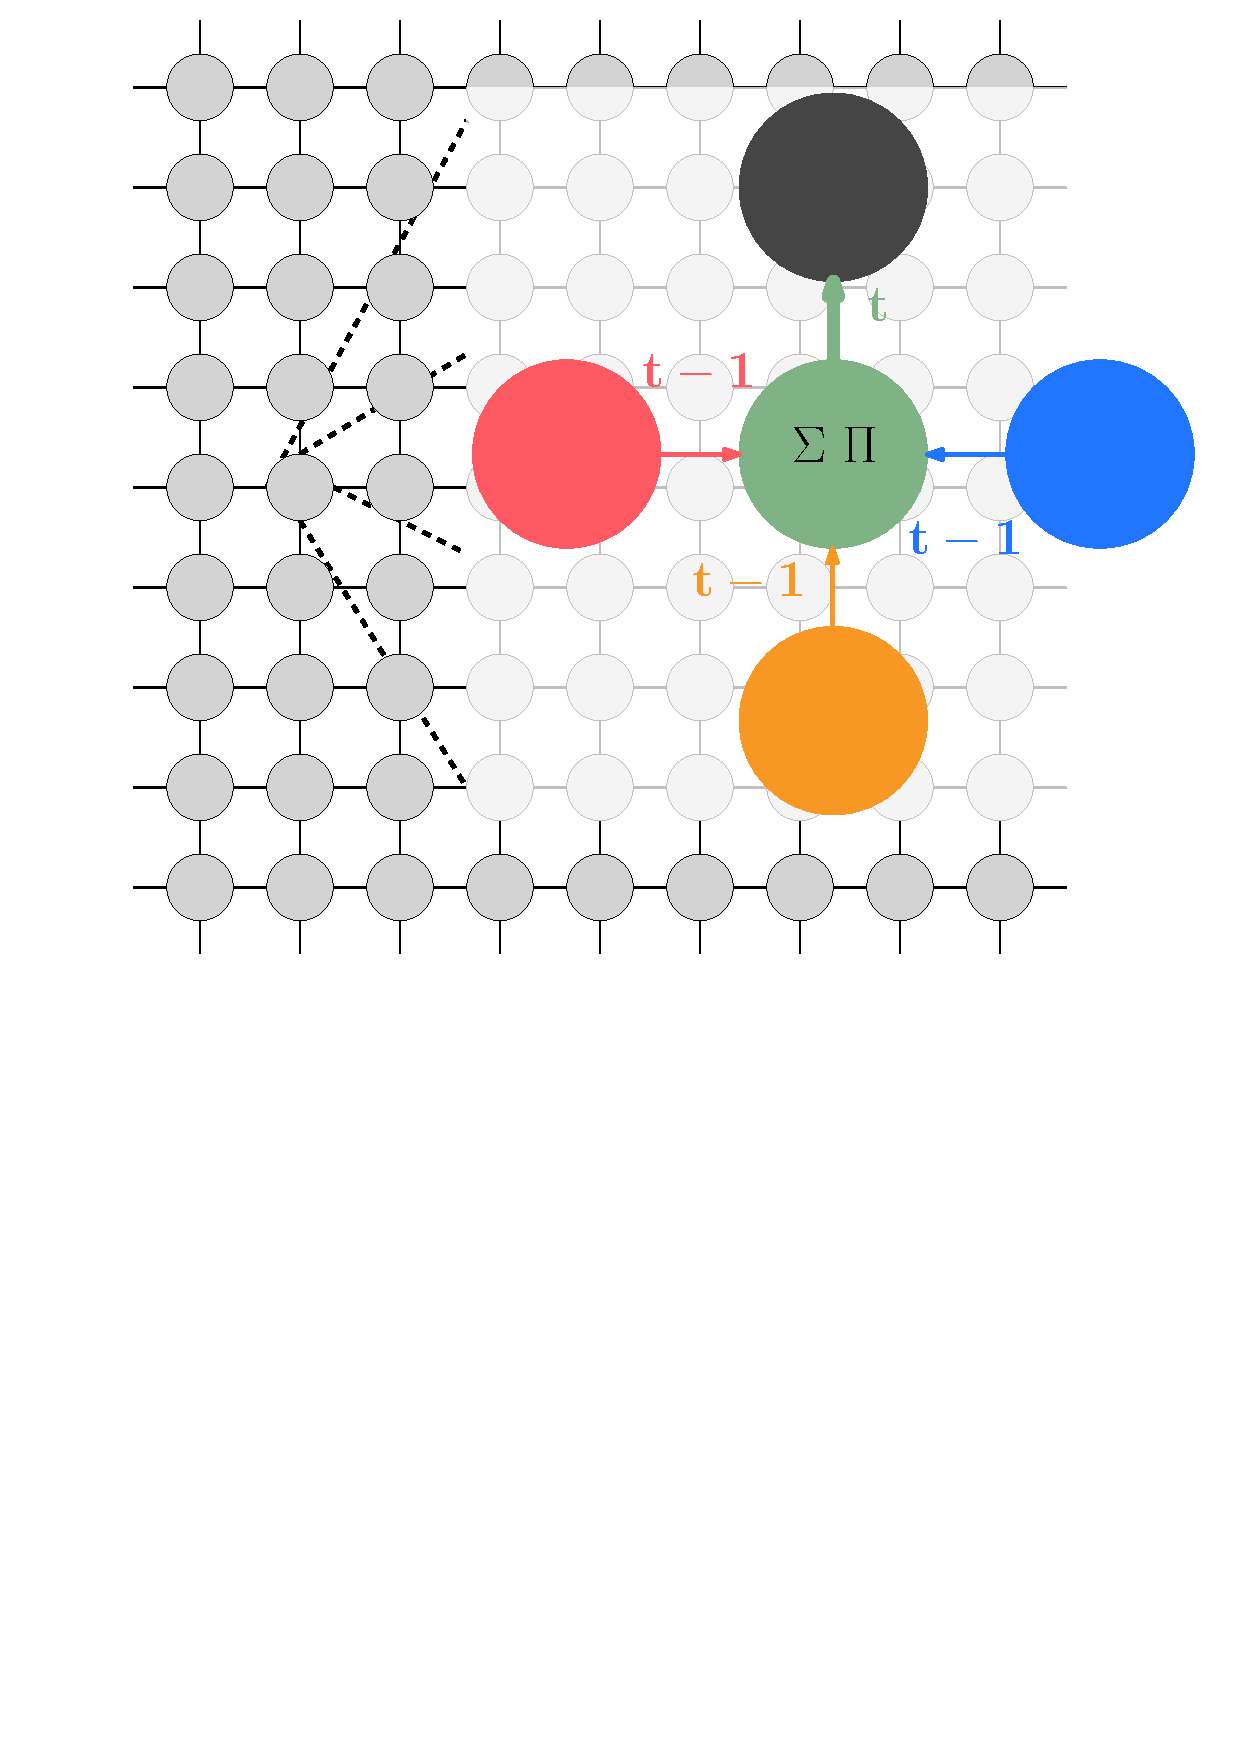
\includegraphics[width=1.0\textwidth]{chapters/litreview/images/bp_diagram_recoloured.pdf}
    \caption{Pictorial representation of the concept behind Loopy Belief Propagation for Stereo Matching. The symbols in the central cell refer to sum-product Belief Propagation, one of the earliest and mostly widely discussed forms of Belief Propagation. Each cell sends a new message to its neighbouring cells at each iteration after in turn having received and processed new messages from the neighbours in the previous iteration. The outgoing message to a given neighbour is computed from the information received from the other neighbours previously, represented here by the three thin and one fat arrow.  Image from \cite{lbpmpsmpic}.}
    \label{fig:bpdiagram}
\end{figure}

Yang \textit{et al.} \cite{Yang2006a} built upon \fxerror*{Explain hierarchical BP}{hierarchical \gls{bp}}, adding in extra steps before and after the \gls{bp} process.  They combine information derived from using the mean shift algorithm \cite{Comaniciu2002}; a colour-weighted correlation method based on Yoon \& Kweon's \cite{Yoon2006} applied to both the left and right images; a left-right consistency check to detect occluded pixels; a plane-fitting process based on Tao \& Sawhney's \cite{Tao2000}; as well as \gls{bp} itself.  While combining these various techniques leads to a highly-accurate disparity map,\footnote{This algorithm achieved the top ranking on Middlebury when it was first introduced.} this approach is \emph{extremely} slow.

Typical \gls{bp} uses the four-connected neighbourhood to define the neighbours of each given node in the grid.  This means that each node passes messages to and from it's immediate neighbours up, down and to the left and right of it in the grid.  Other neighbourhood arrangements are possible though, depending on the underlying model one wants to use.  For example, Tan \textit{et al.} \cite{Tan2017} describe an approach to \gls{bp} where every pixel is considered to be a neighbour of every other pixel.  Messages are weighted according to the distance across the grid between the neighbours, with nearer neighbours having a greater impact upon a pixel's final beliefs.  The major advantage of this approach is that it almost eliminates the need for repeated iterations of message passing.

Ha and Jeong \cite{Ha2016} suggested a different approach for scheduling the messages.  Instead of each pixel repeatedly exchanging messages with its neighbours until a reasonable amount of the grid has been spanned, they start in one of the corners in the image, and sequentially pass messages along two directions until reaching the other corner, repeating this process once for each corner.  The great advantage of this is that in principle one only needs to perform message exchanges in each direction once.  Their implementation still required roughly \SI{3.5}{\second} to complete, however, without returning a significantly more accurate disparity map.\footnote{The authors claimed that their method was \numrange{300}{600} times faster than `standard` \gls{bp}, but they did not specify their stopping condition.  Based on their reported results it appears that they used well over 300 iterations on an image with their standard comparison -- many more than would be reasonable for image sizes likely to be targeted for real-time \gls{sm}.}

Balossino \textit{et al.} \cite{Balossino2007} suggested an alternative formulation to the traditional grid of \gls{lbp}.  Instead, they built a forest of trees, each of which was rooted at the given pixel under consideration, and which has a handful of neighbouring pixels as children.  The attraction of this approach is that it restores the properties of optimality and convergence described in \cite{Pearl1982} for one round of messages up and down each tree.  This advantage is tempered, however, by the necessity of combining results from different trees.  The final accuracy appeared to be worse than with \cite{Felzenszwalb2006}, and there was no reporting of the running time, though it seems unlikely that this approach was fast.

It should be noted that \gls{bp} is \emph{not} regarded as the current top-performing \gls{sm} algorithm.  Tippets \textit{et al.} found c. 2012 that, of algorithms implemented on the CPU, SADL from \cite{VanDerMark2006} was the fastest accurate-enough method, and ADCensus from \cite{Mei2011} was the most accurate, and in fact was described as ``Pareto-optimal'' by Tippets \textit{et al.}  \fxnote{Move this paragraph?}  In terms of \gls{gpu} implementations, the algorithm from \cite{Zhao2011} was the fastest by far (though it only properly worked when observing scenes with motion).  The authors do not state an overall most-accurate \gls{gpu}-based algorithm, but based on Fig. 7 in \cite{Tippetts2016}, it appears that the \gls{gpu} implementation of the ADCensus algorithm from \cite{Mei2011} was again the best.\footnote{Other, faster, algorithms were also discussed, but those required specialist hardware such as \glspl{fpga} or \glspl{dsp}.}  \Gls{bp} \emph{is} amenable to parallelisation (unlike its traditional rival, Graph Cuts \cite{Tappen2003}) and \gls{gpu} implementations, but the main point of interest for it in this work is the fact that it is explicitly built around the concept of independent processing elements exchanging messages.

\begin{anfxwarning}{Top algos on Middlebury}
    Thinking about it, I probably should investigate the current top-performing algorithms on Middlebury, at least the ones which have accompanying publications.
\end{anfxwarning}

\subsubsection{Real-time/resource-constrained \glsentrylong{bp}}
One of the major drawbacks of \gls{bp} as compared to a number of other approaches to \gls{sm} is that a simple naïve implementation is both quite slow, and very memory-intensive.  Slow because of the requirement to perform many iterations, and memory-intensive because \emph{at least} one copy of the data costs and the message estimates for each neighbour must be stored in memory, with the result that a number of values on the order of at least \(O(5XYD)\) are kept in memory, where X and Y are the width and height of the stereo images, and D is the size of the disparity range.

Seeking to derive the comparative benefits of a global stereo algorithm without compromising resource and time requirements too much, there have been a number of attempts at a real-time \gls{bp} algorithm \cite{Liang2011,Perez2010}.

Felzenszwalb \& Huttenlocher \cite{Felzenszwalb2006} made three significant improvements:  i) They demonstrated a way to reduce the complexity of the message update process from \(O(|D|^2)\) to \(O(|D|)\) (where \(|D|\) is the total number of potential disparity labels).  ii) They showed that, because each pixel relies entirely upon the messages received from its neighbours at the previous iteration, only half of the pixels in fact need to be updated in a given iteration, without affecting the final results.  This both halves the number of message computations required for each iteration, but moreover means that only a single copy of the messages need be kept while ensuring that messages computed earlier in an iteration have no impact upon messages computed later.  iii)  They introduced a hierarchical approach, where the first iterations were performed over a much smaller grid, representing an amalgamation of the actual grid, but later iterations would operate over larger and larger grids until reaching the full size.  This had the benefit of propagating information across the grid in a much faster fashion, with relatively little loss in accuracy.  Almost every claimed real-time \gls{bp} algorithm since uses the hierarchical approach.

Notably, Tippetts \textit{et al.} characterised the final algorithm implemented in \cite{Felzenszwalb2006} as Pareto-optimal against almost all other CPU-based \gls{sm} algorithms that they examined, suggesting that there were only five others which provided either better accuracy \emph{or} faster runtimes.  Of course, in the meantime there likely have been improvements in both metrics by newer algorithms.

Yang \textit{et al.} \cite{Yang2006} claimed that they had devised a new approach that would provide a 45x speedup, and boasted that their system could achieve a frame rate of 16 \gls{fps} on a 320 x 240 image with 16 disparity levels.  This claim was largely based, however, in the fact that they used a \gls{gpu} to implement it -- but later stated that they had not yet implemented their method on a \gls{gpu}.  Furthermore, they did not present anything conceptual that had not already been described in \cite{Felzenszwalb2006}. %by Felzenszwalb \& Huttenlocher.

Yu \textit{et al.} \cite{Yu2007} presented a proposed approach for compressing the messages, thus reducing total memory occupied, but it has not proven popular.  This may be because it is not amenable to parallelisation, thus significantly reducing its practicality \cite{Yang2010}.

Yang, Wang \& Ahuja \cite{Yang2010} proposed an approach which they claim needs only constant memory space, regardless of the number of disparities involved, while still returning results that are almost as accurate.  For example, they claim that for an image with 800 x 600 pixels and 300 disparity levels, their algorithm requires only around \SI{9}{\mebi\byte} of memory --- though it is not clear though whether they include storing the computed data costs in that amount or not.  The main element of their approach is that as they move from the coarser levels of the hierarchy, they proportionally reduce the number of disparity labels considered at each level, keeping the total memory required constant.  %This leads to an issue in that, should the true disparity not be selected for inclusion at a reduction, that pixel will never see the correct disparity label assigned to it.  To work around this, they 

Gupta \& Cho \cite{Gupta2012} used 3x3 tiles in their hierarchical method, rather than the usual 2x2.  This meant that their process was somewhat faster overall, and means that at the more coarse levels they need less memory.  The other main differences between their method and previous ones are that they use an `alternative schedule method' borrowed from \cite{Tappen2003}; and they use a different disparity refinement operation as final step.  The results, in terms of accuracy and speed, do not appear to be any better than earlier papers, though.

Xiang \textit{et al.} \cite{Xiang2012} also boasted of a new technique that enabled faster speeds, but again their implementation largely merely borrowed concepts from \cite{Felzenszwalb2006} and used a \gls{gpu}.  They did improve accuracy results, however, by incorporating Yoon \& Kweon's \cite{Yoon2005} adaptive support-weight approach as a post-processing step, with minimal extra computational requirements.

Tan \textit{et al.} \cite{Tan2017} claim that their fully-connected \gls{bp} method is highly-amenable to parallelisation, suggesting it could be implemented to run in real-time, but they do not appear to have done so themselves.

\subsection{\glsentrylong{sgm-glossary}}
This won't really be touched upon in this work anymore, but it might be a good idea to mention/describe it (and perhaps \gls{cp} too), if just so I can mention it again as an obvious future work target.

% \subsection{Noise-Driven Concurrent Stereo Matching}


% \subsection{\label{subsec:concprop}\glsentrylong{cp}}

% \cite{Gong2015,Gong2013a}

% \subsection{Message Passing \glsentrytext{sm} -- other?}
% Look at, e.g.:
% Tan, X. et al. (2017) ‘Efficient Message Passing Methods With Fully Connected Models for Early Vision’, IEEE Transactions on Image Processing, 26(12), pp. 5994–6005. doi: 10.1109/TIP.2017.2750406.
% Ružic, T., Pižurica, A. and Philips, W. (2011) ‘Neighbourhood-consensus message passing and its potentials in image processing applications’, in Astola, J. T. and Egiazarian, K. O. (eds) Image Processing: Algorithms and Systems IX. San Francisco: Society of Photo-Optical Instrumentation Engineers, p. 78700Z. doi: 10.1117/12.872464.
% Ružić, T., Pižurica, A. and Philips, W. (2012) ‘Neighborhood-consensus message passing as a framework for generalized iterated conditional expectations’, Pattern Recognition Letters, 33(3), pp. 309–318. doi: 10.1016/j.patrec.2011.10.014.
% Szeliski, R. et al. (2008) ‘A Comparative Study of Energy Minimization Methods for Markov Random Fields with Smoothness-Based Priors’, IEEE Transactions on Pattern Analysis and Machine Intelligence, 30(6), pp. 1068–1080. doi: 10.1109/TPAMI.2007.70844.
% Thomas, D. et al. (2019) ‘Revisiting Depth Image Fusion with Variational Message Passing’, in 2019 International Conference on 3D Vision (3DV). IEEE, pp. 328–337. doi: 10.1109/3DV.2019.00044.


\chapter{\label{chap:back}Background}
% This review of past work focuses on the main areas of Computer Science that are relevant to this dissertation.  In none of these cases does the review come close to comprehensively covering the entire span of the given area.  It merely tries to cover as much of the relevant recent and classic work as possible, while giving an extremely brief introduction to these areas.  The interested reader who is unfamiliar with any of these topics is strongly advised to refer to the materials cited.

This \lcnamecref{chap:back} summarises some pertinent related topics that are relevant to the central body of this dissertation.  Each is only a short summary, sufficient to communicate key ideas, provide necessary background information, and demonstrate that there are almost always multiple related theoretical concepts and approaches to solving problems.  In none of these cases does the synopsis come close to comprehensively covering the entire span of the given area.  Each part merely tries to introduce and illuminate its topic sufficiently for the purposes of this work.  The interested reader who is unfamiliar with any of these topics is strongly advised to refer to the materials cited.

% See \url{http://forneylab.org/} for something seemingly quite similar to what I'm doing...;  fglib \url{https://github.com/danbar/fglib};  IGraph library \url{https://igraph.org/};  LGNpy \url{https://github.com/ostwalprasad/LGNpy};

This \lcnamecref{chap:back} specifically discusses formal models of concurrent computation, synchronous \& asynchronous communication, \gls{cml} and \gls{mc}.  \Gls{mc} is, in fact, another model of concurrent computation, but given its central position in this work, it is given a dedicated separate \lcnamecref{sec:back:mc}.  The same can be said about \gls{cps}, which is given its own \lcnamecref{chap:tsp}.

\section{\label{sec:back:formalmodels}Formal Models of Concurrent Computation}
The models briefly reviewed in this \namecref{sec:back:formalmodels} are just a small sample of the formal models for computation that have been devised.  An important aspect of each of the ones mentioned below is that they explicitly deal with concurrency in some fashion, thus meriting their (severely abridged) discussion.  Ultimately, \gls{mc} is used as the model of choice for the remainder of the dissertation after this \namecref{chap:back}, but it undoubtedly has been influenced by, or developed contemporaneously with, each of the below.  Indeed, close study of each model inevitably reveals commonalities between them.

\subsection{\label{subsec:back:csp}Communicating Sequential Processes}

\emph{\Gls{csp}} is a \emph{process algebra} and abstract model of concurrent computation put forward by Hoare \cite{Hoare1985,Roscoe2011}.  A typical sequential computation is represented by a \emph{process}.  Processes' \textcquote[][p.~478]{Roscoe2011}{behaviour is described in terms of the occurrence and availability of abstract entities called \textit{events}}.  Should more than one event be available simultaneously for a given process, then one will be chosen non-deterministically.  This choice is internal to the process, and not influenced by, or visible to, other processes.

Concurrency is introduced by the existence of multiple processes.  In general, the processes continue independently, responding to events as they come.  Should a particular event appear in the alphabet of multiple processes, however, then all processes \emph{must} choose to participate in that event at the same time.  Should all processes involved make such a choice, they engage in a synchronous multi-way atomic synchronisation (hence ``communicating'').  \Gls{csp} has provided significant inspiration for concurrency design in a number of programming languages, notably including Ada \cite{Defense1983,Taft2013}, Occam \cite{Elizabeth1987}, Google's Go \cite{Meyerson2014} (not to be confused with the earlier language Go! \cite{Clark2004}, which itself was explicitly designed for concurrency) and \gls{cml} \cite{Reppy2011} (see further \vref{sec:back:cml}).  An especially interesting practical application of \gls{csp} itself is finding flaws -- and fixes to the flaws -- in information security protocols \cite{Roscoe1995,Lowe1996,Koltuksuz2010}.

\subsubsection{\(\pi\) Calculus}
\(\pi\) calculus was created by Robin Milner and associates in the early 1990s, building upon \gls{csp}.  Milner appreciated \gls{csp}, which advanced concurrency models by explicitly incorporating \emph{synchronised} interaction, something his earlier Calculus for Communicating Systems \cite{Milner1980} had lacked  \cite{Milner1993}.  Milner still regarded \gls{csp} as incomplete, however, in that it had no support for the concept of `mobility' --- \ie{} the ability of the system to reconfigure itself during operation.  In the context of \(\pi\) calculus, this is achieved by passing references to links between processes via other links, thus enabling a dynamic communication system. \(\pi\) calculus was created as an attempt to build upon earlier systems but present a complete calculus of concurrent computation, in much the same way that Lambda Calculus \cite{Barendregt1984} is a complete calculus for sequential computation.\footnote{Milner also noted that sequential computation is a special case of concurrent computation \cite{Milner1993}.}

Both \gls{csp} and \(\pi\) calculus are effective for modelling concurrent systems (see \eg{} \cite{Roscoe2011}).  They have a drawback, however, in that they tend to be very verbose.  Specifications of behaviour for processes are intertwined with the descriptions of processes' states.  They are effective for specifying a system formally, and verifying the behaviour of said system by defined reductions (see \eg{} \cite[Ch.~3.2]{Varela2013}), but for larger systems the notational burden can make it difficult to understand what each process can and will do.

\subsection{\label{subsec:back:actors}\texorpdfstring{\Glspl{actor}}{Actors}}
The \emph{\gls{actor}} model was introduced by Carl Hewitt \cite{Hewitt1973} and substantially further developed for practical programming use by Gul Agha and others \cite{Agha1986,Agha1997}.  Much like \gls{csp} \& its cousins, the \gls{actor} model is based around the concept of sequential, separate but communicating processes which exchange messages.  Again, the processes make decisions independently and proceed based on their communications.  A key difference, however, is that in the \gls{actor} model the message exchanges are \emph{asynchronous}.  Each \gls{actor} has its own \emph{mailbox}, and may send messages to other \glspl{actor} so long as it knows their identity (which is equivalent for this purpose to a concept of a postal address for the \gls{actor}), \emph{but does not wait at all for a response before proceeding}.  Moreover, for \glspl{actor}, the \emph{only} way to communicate with one another is to know the intended recipient's identity/address.  Logical shared memory is explicitly disallowed,\footnote{It is entirely possible in practice, of course, to implement an \gls{actor} system on a shared memory system, but the model expressly forbids any notion of a resource shared in any fashion besides \glspl{actor} requesting a result from another \gls{actor} who has exclusive access to the resource.} which prevents changing who an \gls{actor} communicates with simply by \eg{} changing the holder of a channel endpoint, but also means that actors can be distributed by a runtime without (directly) affecting the practical programming.

The \gls{actor} model is popular for concurrent programming, possibly owing to its intuitive concept.  The fact that communication is asynchronous makes \glspl{actor} much more suitable for modelling distributed systems without shared memory than \gls{csp} or similar --- \glspl{actor} can send messages and proceed without (necessarily) needing to wait for a response, instead continuing forward based on the messages they have received.  By contrast, a typical distributed system with synchronous communication would have prohibitive time costs, given the relative slow speed of typical links between distributed computers as compared to their capacity for local processing.  Many \gls{actor} systems have been implemented for different programming languages (\eg{} \cite{Varela2001,Srinivasan2008,Charousset2016,Bernstein2016}), and in fact it is a core component, and perhaps largely responsible for the success, of Erlang/OTP \cite{Armstrong2010,Armstrong2013,Vinoski2012}.  A relatively new language, Pony \cite{Clebsch2015,Clebsch2017}, takes this even further.

\Glspl{actor}, when used for non-trivial real-world software, have been criticised at times \eg{} \cite{Welsh2013,Stucchio2013}.  While some of the criticisms described are implementation-specific (relating to Akka, a Scala \gls{actor} library), a common thread is that \glspl{actor} do not compose well.  This has the negative consequence that it is difficult to combine an \gls{actor} with anything else to create a new abstraction, and can require extensive modifications in source code to make relatively simple logical changes.

\subsection[GAMMA, the Chemical Abstract Machine, and Join Calculus]{\(\Gamma\), the Chemical Abstract Machine, and Join Calculus}

\subsubsection{\(\Gamma\)}
\citeauthor{Banatre1993} \cite{Banatre1993}, described the \(\Gamma\) (\emph{GAMMA}) ``language'', which uses the multiset as its singular data structure.  The originators stated that their goal with \(\Gamma\) was to create a \enquote{a program structuring tool} focusing on \enquote{logical parallelism} (which seems to be their name for concurrency), rather than creating a working programming language.  Indeed, they acknowledged that translating multiset transformations into programs working on existing electronic computers of the time may prove challenging.  The principal aim was to provide a facility for program designers to state at a high-level the intended transformations, avoiding imposing any ordering on the processing and instead permitting as much concurrency as possible:  \textcquote[][p.~102]{Banatre1993}{our high level of abstraction eliminates unfortunate sequential biases.}  In essence, \(\Gamma\) takes an extreme declarative approach.

Perhaps the largest drawback of \(\Gamma\) is its lack of any form of central control.  All computation is performed through local operations, while \textcquote[][p.~108]{Banatre1993}{the only known solutions to certain problems rely on control decisions involving the whole state of the computation.}  The first problem of such that \citeauthor{Banatre1993} point to is the \gls{gcp} (which is solved in linear time in \cref{chap:gcol} in the present dissertation).  While such problems \emph{can} be solved, expressing the solutions would likely be more, rather than less, complicated than in other systems.  Another criticism that can be levelled at \(\Gamma\) is its lack of formality around its data structure.  Multisets are used, but there is no clear foundation underpinning them.  Rather, in \cite{Banatre1993} both integers and tuples are used as the set elements without any consideration of how they might be constructed or represented.  This is probably appropriate for the extreme high level of \(\Gamma\), but it could impede conversions of its programs to lower level languages more suited to working implementations.

\subsubsection{The Chemical Abstract Machine}
\citeauthor{Berry1992} devised the idea of the \emph{\gls{cham}} \cite{Berry1992}, directly inspired by the concepts from, and building upon, \(\Gamma\).  The parallels between the \gls{cham} and \gls{mc} are clear.  Indeed, the \gls{cham} includes a concept of \glspl{compartment} created by membranes.  Moreover, in his foundational exposition of \gls{mc} \cite{Paun2000}, \citeauthor{Paun2000} directly cites \(\Gamma\) \cite{Banatre1988} and \gls{cham} \cite{Berry1992}.

\(\Gamma\) had a loose notion of being rooted in chemistry, but \gls{cham} significantly adds to the rigour of the analogy, introducing concepts such as molecules composed of atoms, where a system is a collection of such molecules and may be heated or cooled to change the molecular composition.  Where \cite{Banatre1993} made clear the potential of multiset transformations for concurrency, \cite{Berry1992} adds formalisms that enable much more precise specifications of the process of the transformations, without sacrificing the extreme levels of concurrency possible.  The authors demonstrate this fact by showing that \glspl{cham} \enquote{can implement known models of concurrent computation}, including CCS \cite{Milner1980}, mobile processes \cite{Milner1991} and concurrent lambda calculus \cite{Boudol1989}.

\subsubsection{Join Calculus}
Where the \gls{cham} was a development of \(\Gamma\), join calculus is in turn a development of the \gls{cham}.  Join calculus -- created in the 1990s by \citeauthor{Fournet1996} \cite{Fournet1996,Fournet2002} and using the \gls{cham} as its underlying ``machine'' (although, it actually originally targeted \(\pi\) Calculus before switching to the \gls{cham} as a much better fit for its core concepts \cite{Fournet2002}) -- is arguably the most similar in practice of all the models discussed in this \namecref{sec:back:formalmodels} to \gls{mc}.  There are clear common elements between join calculus and \gls{cps}, including heavy use of pattern matching and communication via channels.  Even its reaction rules closely resemble the typical style of rules found in most flavours of \gls{ps} (see \cref{sec:back:mc,chap:cpsystems}).

\citeauthor{Fournet2002} specifically describe join calculus as \textcquote[][p.~269]{Fournet2002}{an attempt to provide language support for asynchronous, distributed, and mobile programming.}  Join calculus has proved fruitful for assisting in the design of new concepts in practical programming, including JoCaml \cite{Fournet2003} (essentially an implementation in OCaml of join calculus as a programming system), Joinads \cite{Petricek2011}\footnote{See also \url{http://tryjoinads.org/docs/use/joins.html}.} and Reagents \cite{Turon2012}.  Despite this utility, however, join calculus seems largely to have been neglected by those outside the theoretical computer science and programming languages communities and appears to have been entirely unused in more recent years.  Later work building on this dissertation could well benefit from an attempt to use join calculus, but it appears less likely to be immediately fruitful than using \gls{mc}.

\subsection[Brane- and Kappa-Calculus]{Brane- and \(\kappa\)-Calculus}
\subsubsection{Brane Calculus}
Brane Calculus\footnote{\citeauthor{Cardelli2005} actually referred to it as Brane \emph{Calculi}, given that he saw it as a family of related systems, but Calculus is used here for consistency with the other described models.} might appear, \foreign{prima facie}, to be the closest relative to \gls{mc} of all the models presented in this \namecref{sec:back:formalmodels}.  The subtitle given to its exposition is \enquote{Interactions of Biological Membranes} \cite{Cardelli2005}.  Both models are undeniably grounded in concepts of cellular biology, with particular emphasis on the cell's membranes.  Both focus heavily on the nesting of those membranes, and movement of items among them.  In actuality, they are dissimilar.

Brane Calculus is as much a system for modelling certain biological processes as it is a computational system.  Importantly, it means that the primitives chosen for it are relatively biologically realistic, and likely much more feasible to implement physically using biology.  While that has some clear potential benefits, it also tends to make even relatively simple systems somewhat difficult to follow.

Brane Calculus also treats its membranes somewhat differently.  In \gls{mc} (certainly \gls{clps}, at least), membranes are used primarily to separate regions of computation and avert undesired interactions between the contents of \glspl{compartment}.  In Brane Calculus, however, much of the processing occurs \emph{on} the membrane itself: \textcquote[][p.~257]{Cardelli2005}{Membranes are not just containers, they are coordinators and active sites of major activity.}  Brane Calculus seems like a promising potential target for an ``intermediate language'' in between \gls{ps} and real biological implementations, but also seems much less useful for expressing the core essence of general computations than \gls{mc}.

\subsubsection{\(\kappa\)-calculus}

Similarly to Brane Calculus, \(\kappa\)-calculus \cite{Danos2004} was introduced as a formal representation of an aspect of cellular biology grounded in prior work in theoretical computer science on concurrent languages.  The focus in \(\kappa\)-calculus is predominantly upon protein interactions, rather than membranes as with Brane calculus: \textcquote[][p.~70]{Danos2004}{Our language idealizes protein-protein interactions, essentially as a particular kind of graph-rewriting}.  This protein focus is demonstrated in \cite{Danos2004} with an example describing part of the digestion process that occurs inside \textit{E.Coli} bacteria, the \enquote{lactose operon}.

The development of \(\kappa\)-calculus may have remained more firmly grounded in traditional concurrency theory than Brane Calculus.  Notably, \citeauthor{Danos2004}, in \textcquote[][p.~76]{Danos2004}{a side observation perhaps only of interest for Concurrency theorists} comment upon their use of \enquote{the ordinary material of process algebras}, pointing out that they use only a minimal subset of the usual operations.  Furthermore, they demonstrated that their simpler (in terms of allowed protein reactions) language \(m\kappa\)-calculus could simulate \(\pi\) calculus, meaning that they could translate systems created in \(\kappa\)-calculus to \(\pi\) calculus and then use programmatic implementations of \(\pi\) calculus, such as Nomadic Pict \cite{Unyapoth2001}, to run those systems on electronic computers.  While this shows that \(\kappa\)-calculus could be used to model solutions to arbitrary problems, it still suffers from the same problem as Brane Calculus.  The modelling for even relatively simple systems quickly becomes quite complex and difficult to read, diminishing the utility of \(\kappa\)-calculus for exploring alternative solutions to known problems in computer science.

\subsection{\label{sec:back:othermodels}Other Models}

\subsubsection{Petri Nets}
Perhaps the earliest formalised model of concurrent computation still in wide use is the \emph{Petri net} \cite{Dennis2011}, first conceived of by Carl Petri to describe chemical processes \cite{Petri2008}.  A basic Petri net consists of places, tokens and transitions, where tokens move between places via arcs and all places are separated by transitions (and \viceversa).

The main weakness of classical Petri nets is that they require the definition of a fixed system from the outset, and do not easily permit the evolution of the system during ``runtime'' as appropriate.  Of Petri nets, \citeauthor{Varela2013} says \textcquote[][p.~36]{Varela2013}{Petri nets \textelp{} in the \textelp{} form described \textins{in \cite{Varela2013}}, \textelp{} are not able to model the dynamicity of concurrent software\textins{.}  \textelp{} Petri nets \textelp{} do not support the compositional reasoning afforded by more modern models of concurrency.}

\subsubsection{\label{sec:back:pram}Parallel Random Access Machines}

\emph{\Glspl{pram}} are a model for concurrent computation arguably closer to the operation of real electronic computers than the others described above.  \citeauthor{JaJa2011} defines a \gls{pram} as \textcquote{JaJa2011}{an abstract model for parallel computation which assumes that all the processors operate synchronously under a single clock and are able to randomly access a large shared memory. In particular, a processor can execute an arithmetic, logic, or memory access operation within a single clock cycle}.  Unlike the process algebras described above, the \gls{pram} model does not, in general, impose a particular way to describe a \gls{pram} algorithm, making it sometimes quite seful in developing parallel algorithms.

\Glspl{pram} developed as a natural extension to random access machines (RAMs), which, as the name suggests, provide a model that is reasonably close to typical uniprocessor electronic computers.  A \gls{pram} is a collection of processors operating synchronously (\ie{} on the same clock), each labelled with a unique identifier, and with access to a global shared memory.  Processors may operate independently of each other, but many described \gls{pram} algorithms in fact operate in a \emph{single-program multiple-data} fashion where all processors follow the same program and so are only semi-independent, at best.  These attributes mean that a \gls{pram} often looks quite similar (at a superficial level, at least) to the operation of a typical \gls{gpu}.  The systems described in \cref{chap:nmp} also bear more than a passing resemblance to \glspl{pram}.
%-------------------------------------------------------
\section{\label{sec:back:syncasync}Synchronous and Asynchronous Messaging in Distributed Algorithms}
%-------------------------------------------------------

This dissertation uses the standard timing models in distributed algorithms \cite{Lynch1996} for messaging where relevant.  For reference, the most important relevant concepts are explained and illustrated below.  For more on the topics discussed in this \namecref{sec:back:syncasync}, the interested reader is referred to \cite{Fokkink2013,Lynch1996,Tel2000}.

\subsection{Rounds}
Under both synchronous and asynchronous messaging, all processes work in \emph{rounds} (sometimes also referred to as \emph{macro-steps}).  A round consists of three repeating sequential sub-steps:
\begin{enumerate}
    \item \emph{\textsf{Receive}}:  receive one or more incoming messages
    \item \emph{\textsf{Process}}:  perform any requisite local computations as induced by the received messages, and update the local state
    \item \emph{\textsf{Send}}:  send out new messages as appropriate based on the processing from the previous step
\end{enumerate}
This applies only to messaging between processes.  For systems with a solitary process, there is no meaningful concept of rounds because the process will essentially remain in the \textsf{process} sub-step.  \Ie{} a lone process will continue working without messaging until the system halts (if ever).

\subsection{Synchronous Messaging}
Under the synchronous model, all processes proceed in lock-step.  They may carry out the sub-steps at different speeds, but begin and end rounds together.  When considering timing of messaging, there are two standard approaches:  to consider the \textsf{process} sub-step as taking one time unit and the transit time -- the time between when the message is sent by the sender and when it is received by the recipient -- taking zero time units; or, to consider the \textsf{process} sub-step as taking zero time units and the transit time taking one time unit.

\subsection{Asynchronous Messaging}
Under the asynchronous model, there is (unsurprisingly) no natural synchronisation between processes.  All processes proceed through the sub-steps at their own pace.  The \textsf{process} sub-step is considered to take zero time units, and message transit times are considered to take any number of time units.  Alternatively, by normalisation, while the \textsf{process} sub-step still takes zero time units, message transit times take somewhere between zero and one (inclusive) time units.  This makes the second synchronous approach a special case of the asynchronous approach.  The asynchronous model is similar to the theoretical \gls{actor} model.

\subsection{Echo}
To illustrate the difference between the synchronous and asynchronous scenarios, consider the illustrations in \cref{fig:back:echosync,fig:back:echoasync}.\footnote{These figures were created by Dr. Radu Nicolescu, and have been reproduced here with his permission.}  The \textsf{echo} algorithm \cite[Ch.~4.3]{Fokkink2013} is used to establish a spanning tree over a graph of nodes/processes, in this case rooted at node 1.  The algorithm works in two phases, named \emph{broadcast} and \emph{convergecast}.  \textsf{Echo} starts in the broadcast phase with an initiator node sending out a broadcast message to each of its neighbours.  Each of those recipients then marks the sender as its parent, sends a broadcast message to every other one of its neighbours, then waits to receive a broadcast message from each of those other neighbours.  This pattern repeats across the graph.  Once the response broadcast messages are received, each node then sends a convergecast message back to its parent.  This carries on until finally the initiator receives the convergecast messages back from its neighbours.

In \cref{fig:back:echosync,fig:back:echoasync}, the first green node is the initiator, and each other node turns green when it receives its first message.  Edges between nodes turn into green arrows when a node chooses its parent.  The direction of the arrow points to said parent.  Red arrows indicate the direction of travel for a broadcast message, while blue arrows indicate the direction of travel for a convergecast message.  Solid red \& blue arrows indicate that a message is received in that round by the recipient, while a dashed line indicates that the message is still in transit.

\begin{figure}[htbp]
    \centering
    \subcaptionbox{Round Zero}{\includegraphics[width=0.32\textwidth]{chapters/background/images/echo/sync/notext_f0_0.pdf}}
    \subcaptionbox{Round One}{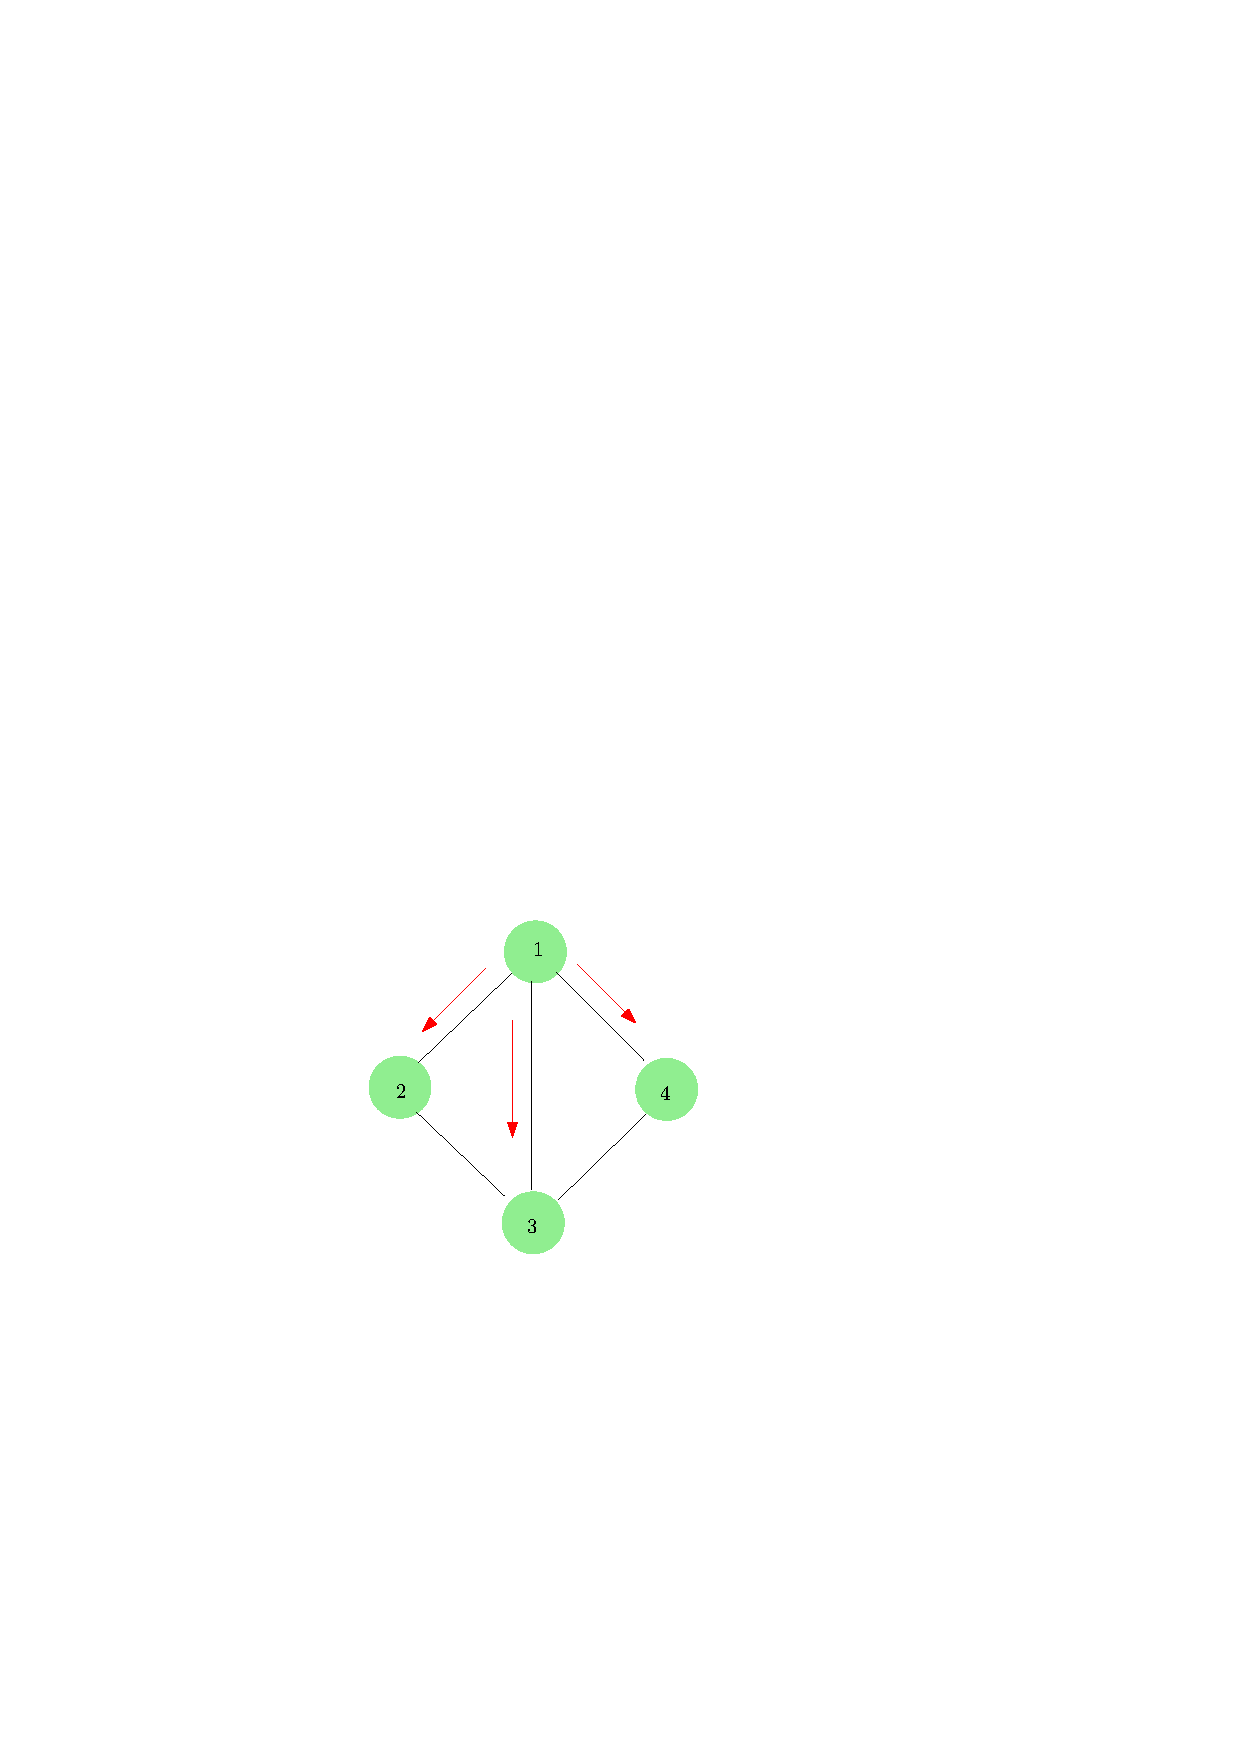
\includegraphics[width=0.32\textwidth]{chapters/background/images/echo/sync/notext_f0_1.pdf}}
    \subcaptionbox{Round Two}{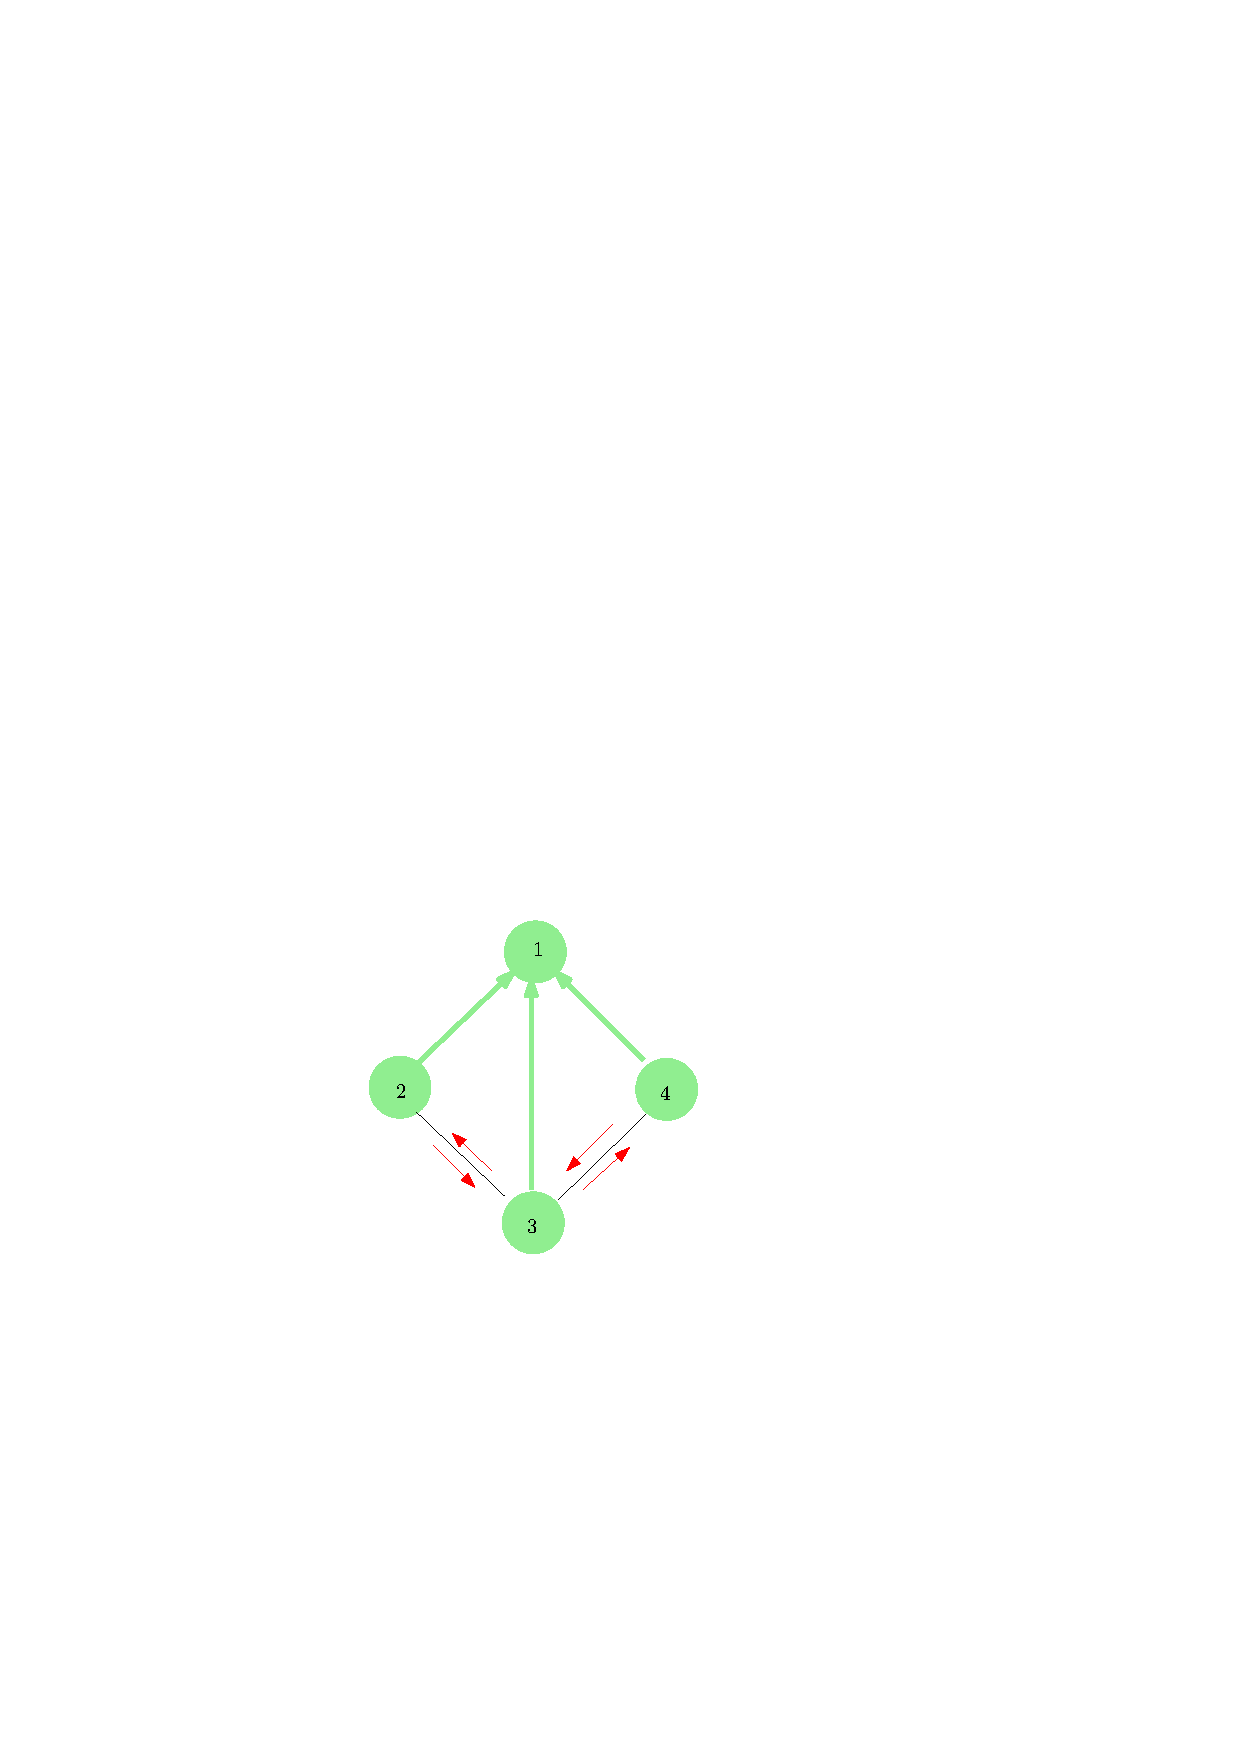
\includegraphics[width=0.32\textwidth]{chapters/background/images/echo/sync/notext_f0_2.pdf}}
    \subcaptionbox{Round Three}{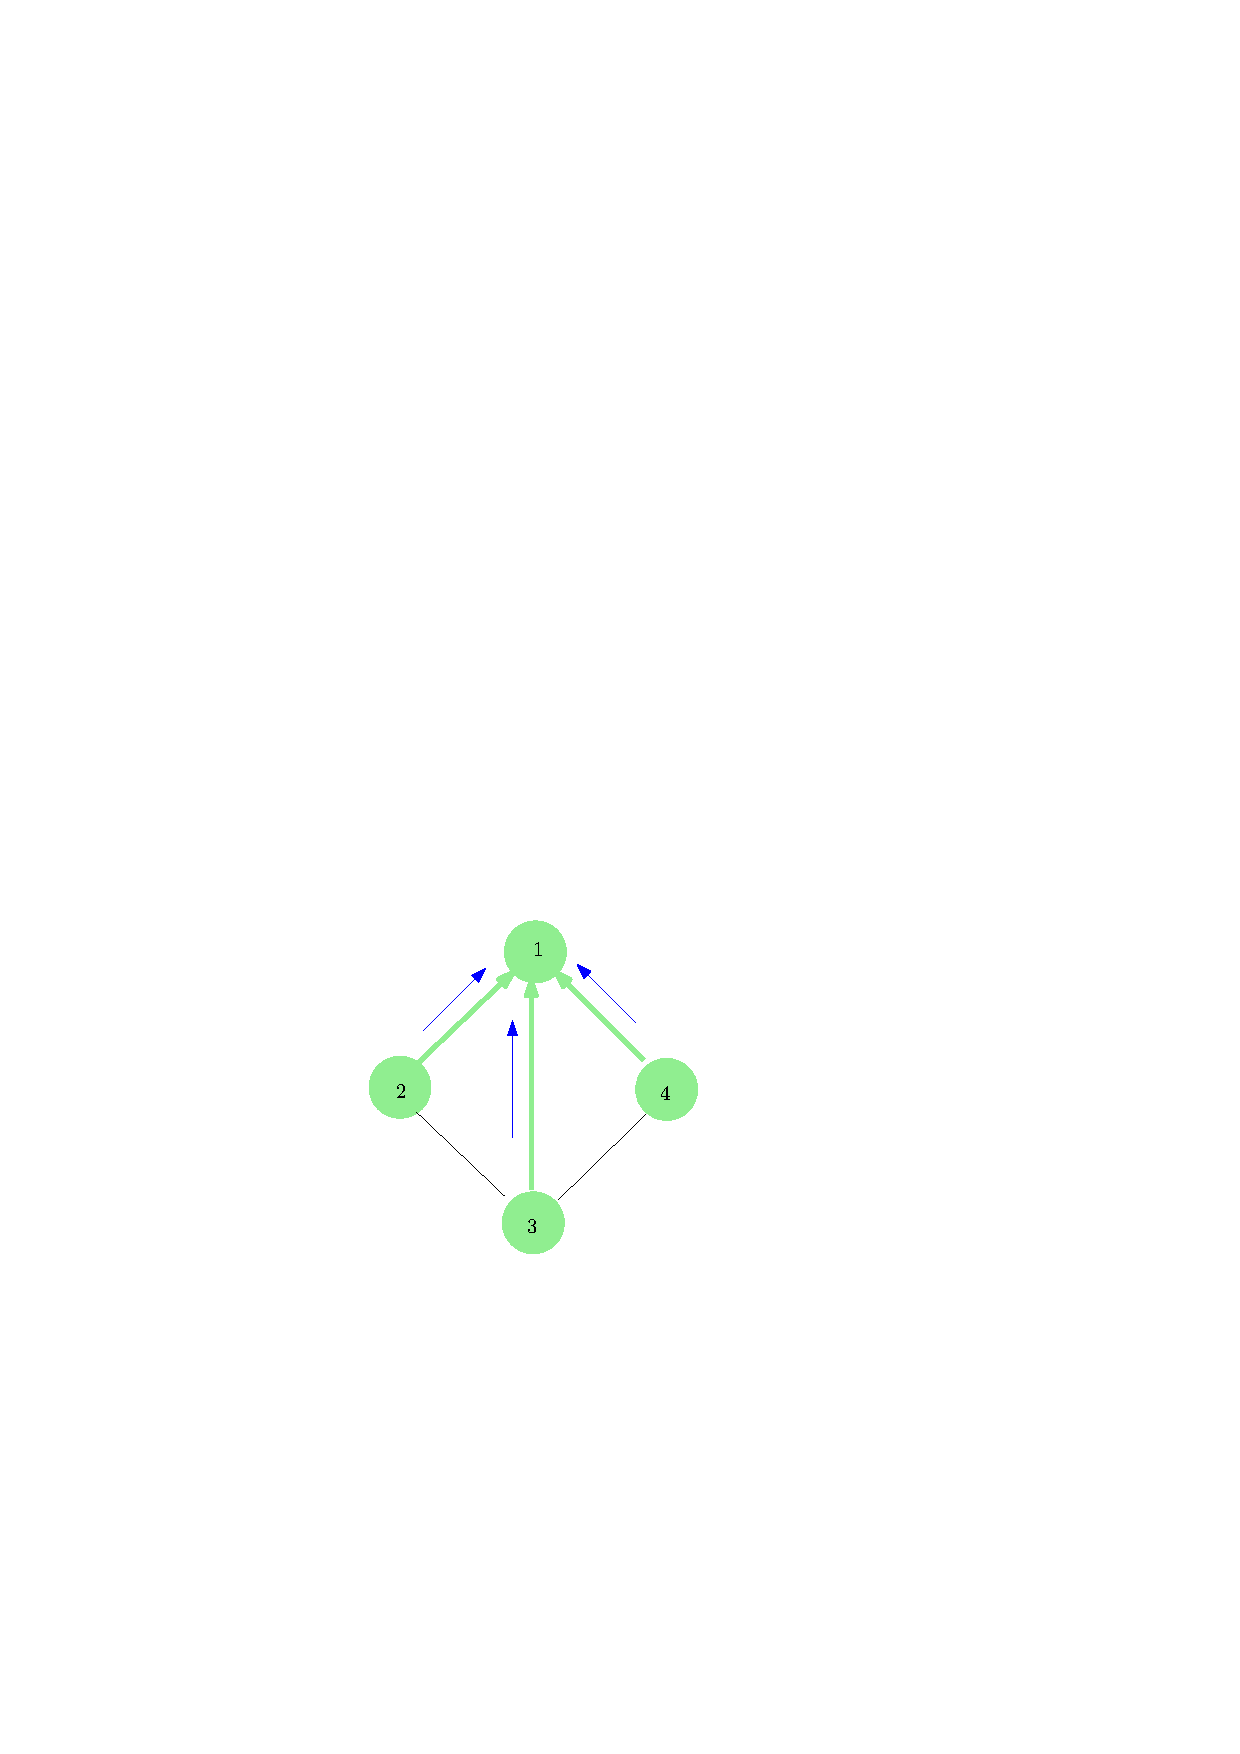
\includegraphics[width=0.32\textwidth]{chapters/background/images/echo/sync/notext_f0_3.pdf}}
    \caption[Progression of the synchronous \textsf{echo} algorithm]{Progression of the synchronous \textsf{echo} algorithm, starting from round zero before any messages are sent.  Arrows in red mean broadcast messages, while arrows in blue mean convergecast messages.}
    \label{fig:back:echosync}
\end{figure}

\begin{figure}[htbp]
    \centering
    \subcaptionbox{Round Zero}{\includegraphics[width=0.32\textwidth]{chapters/background/images/echo/async/notext_f0_0.pdf}}
    \subcaptionbox{Round One}{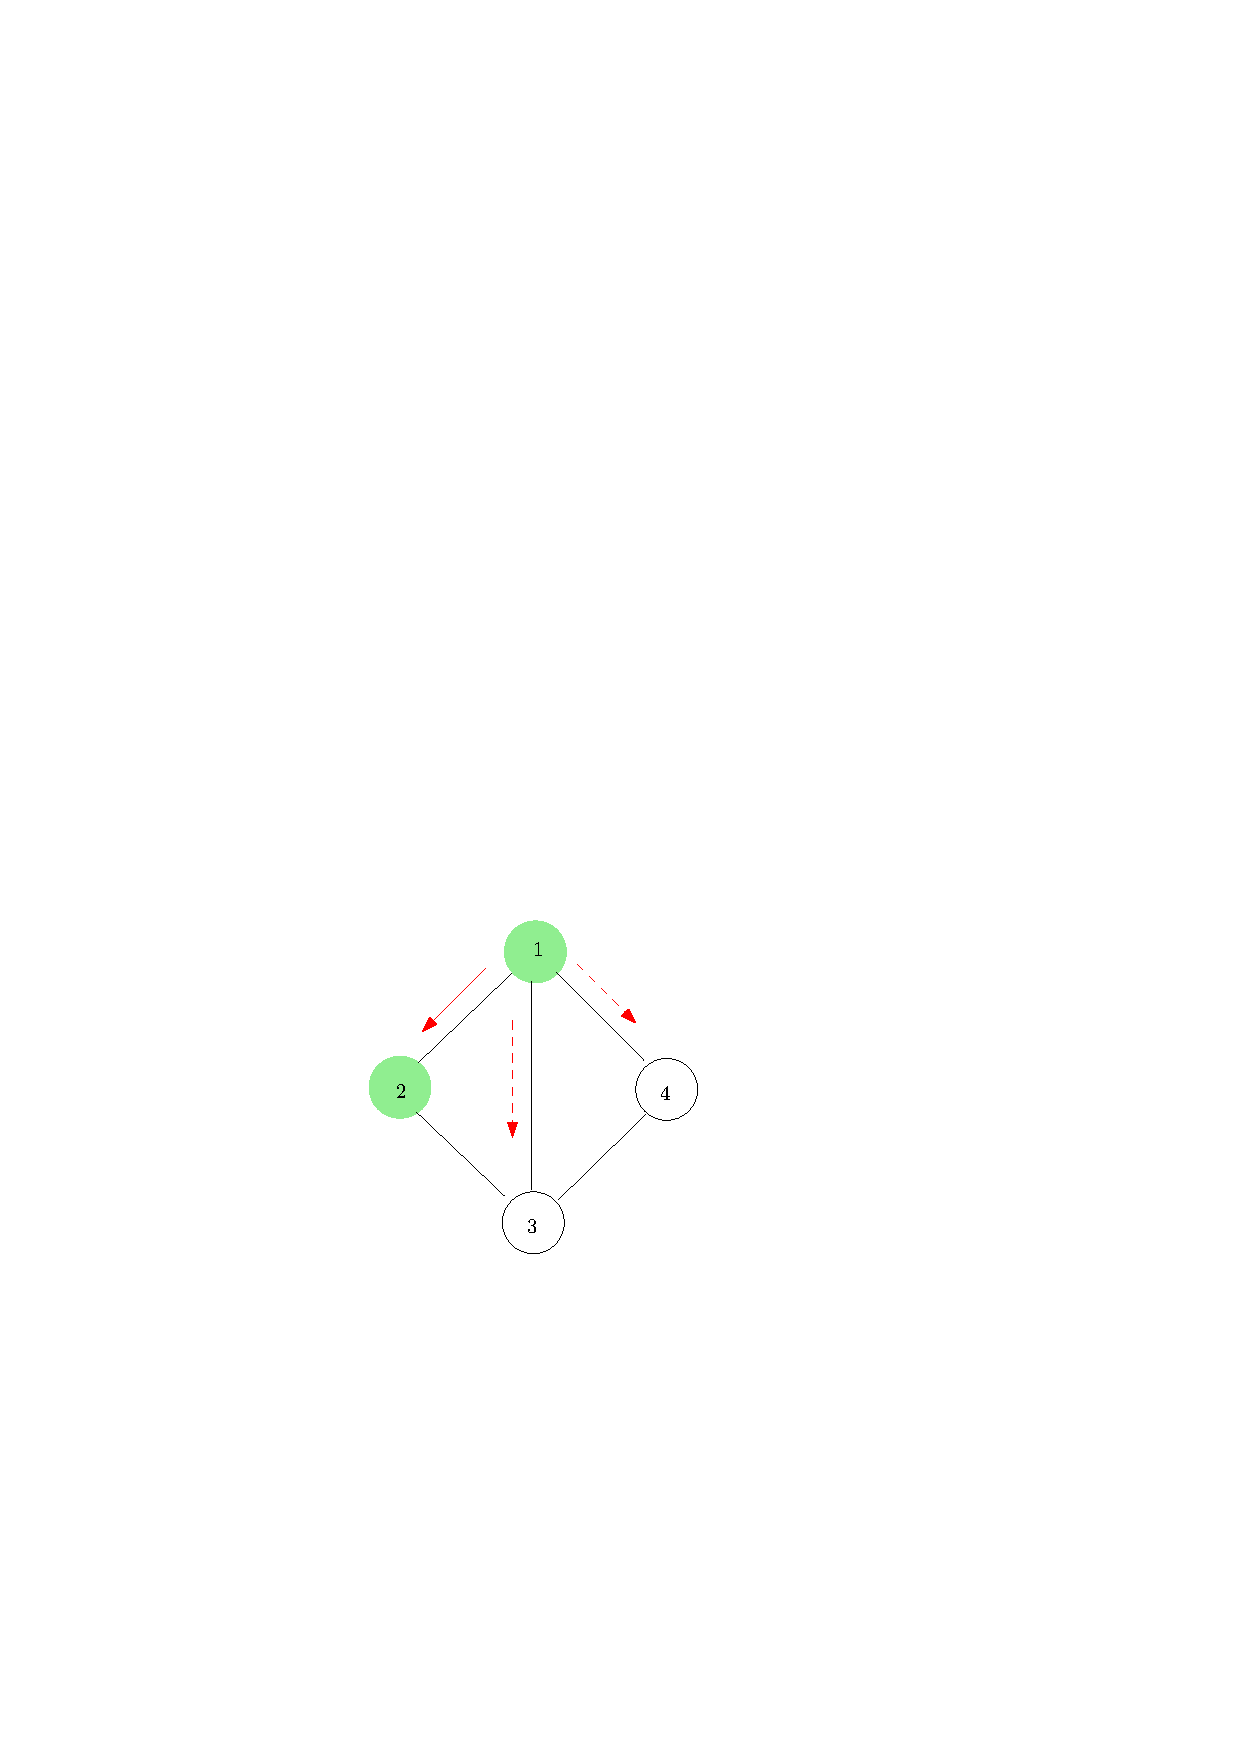
\includegraphics[width=0.32\textwidth]{chapters/background/images/echo/async/notext_f0_1.pdf}}
    \subcaptionbox{Round Two}{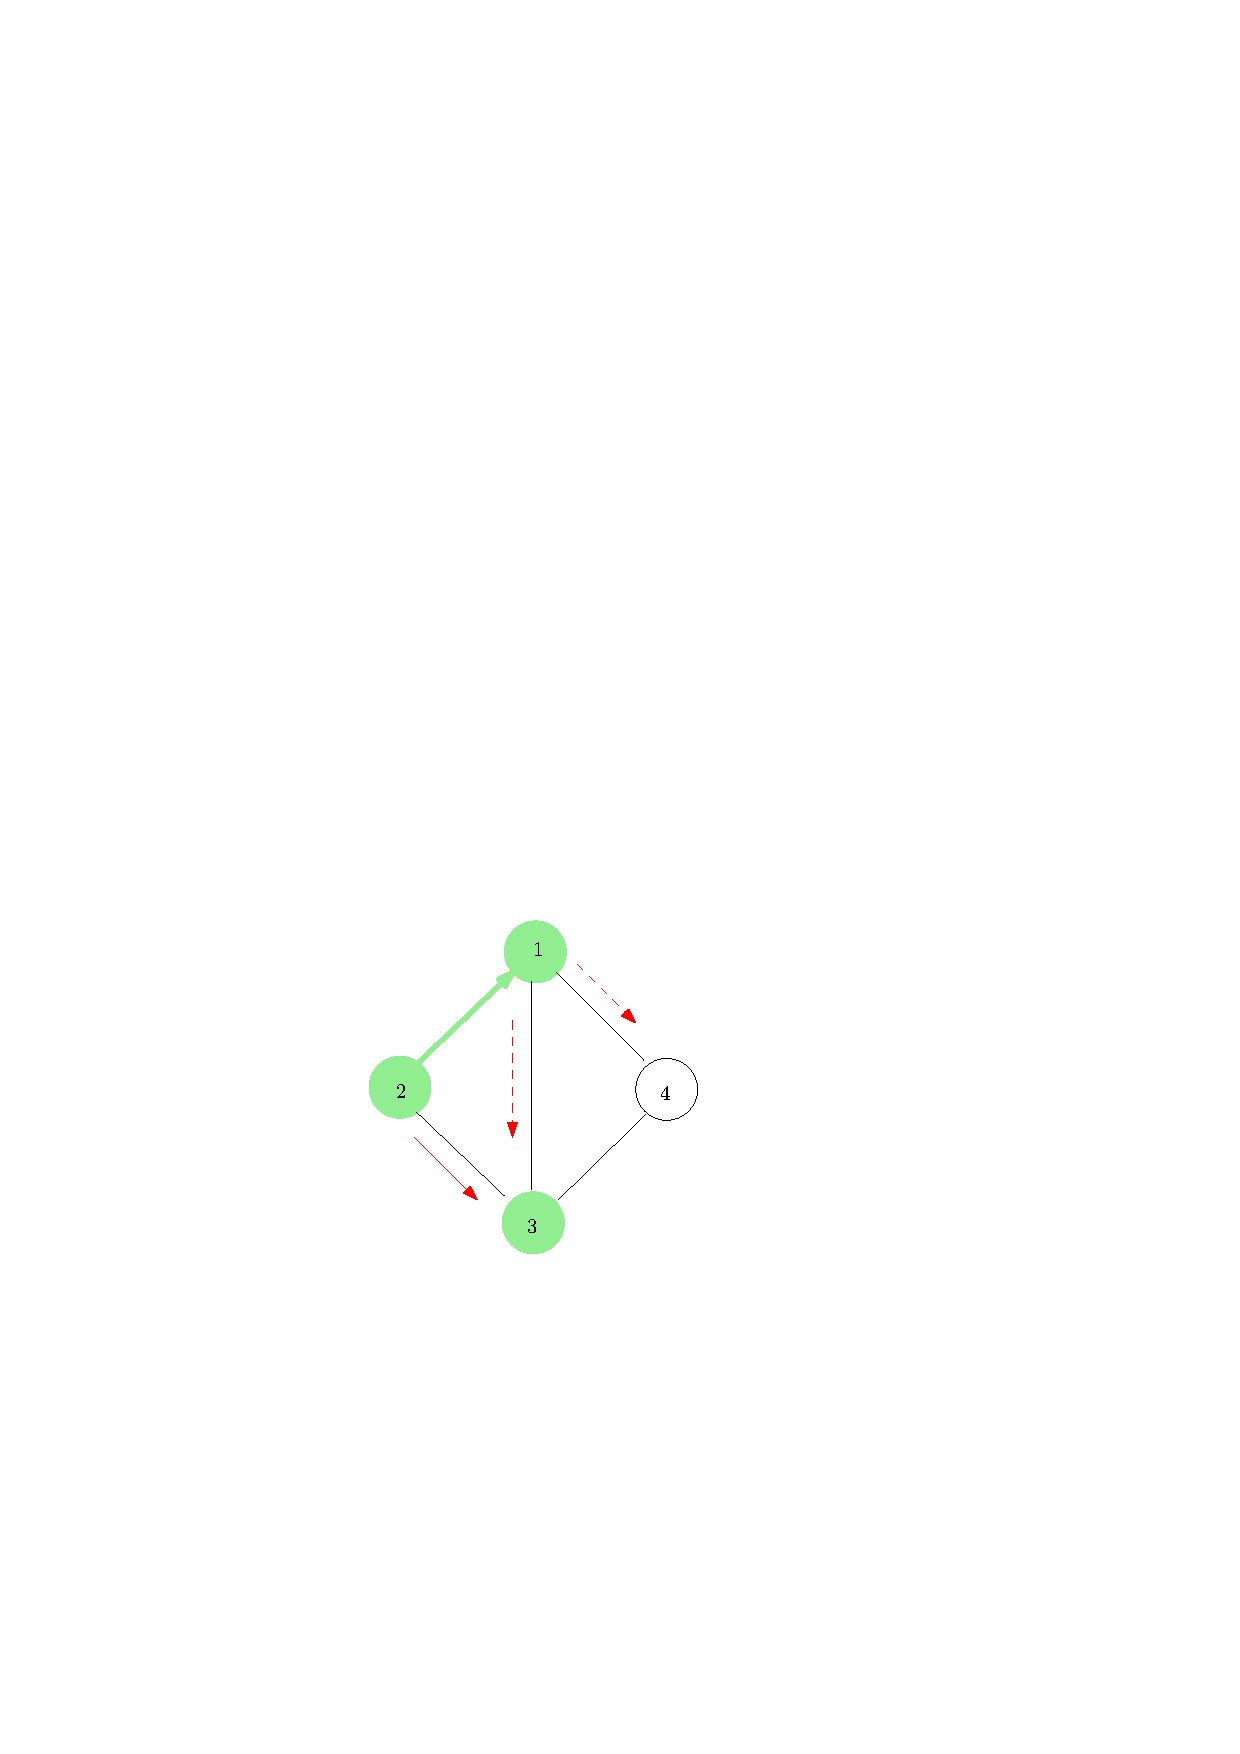
\includegraphics[width=0.32\textwidth]{chapters/background/images/echo/async/notext_f0_2.pdf}}
    \subcaptionbox{Round Three\label{fig:back:echoasync:3}}{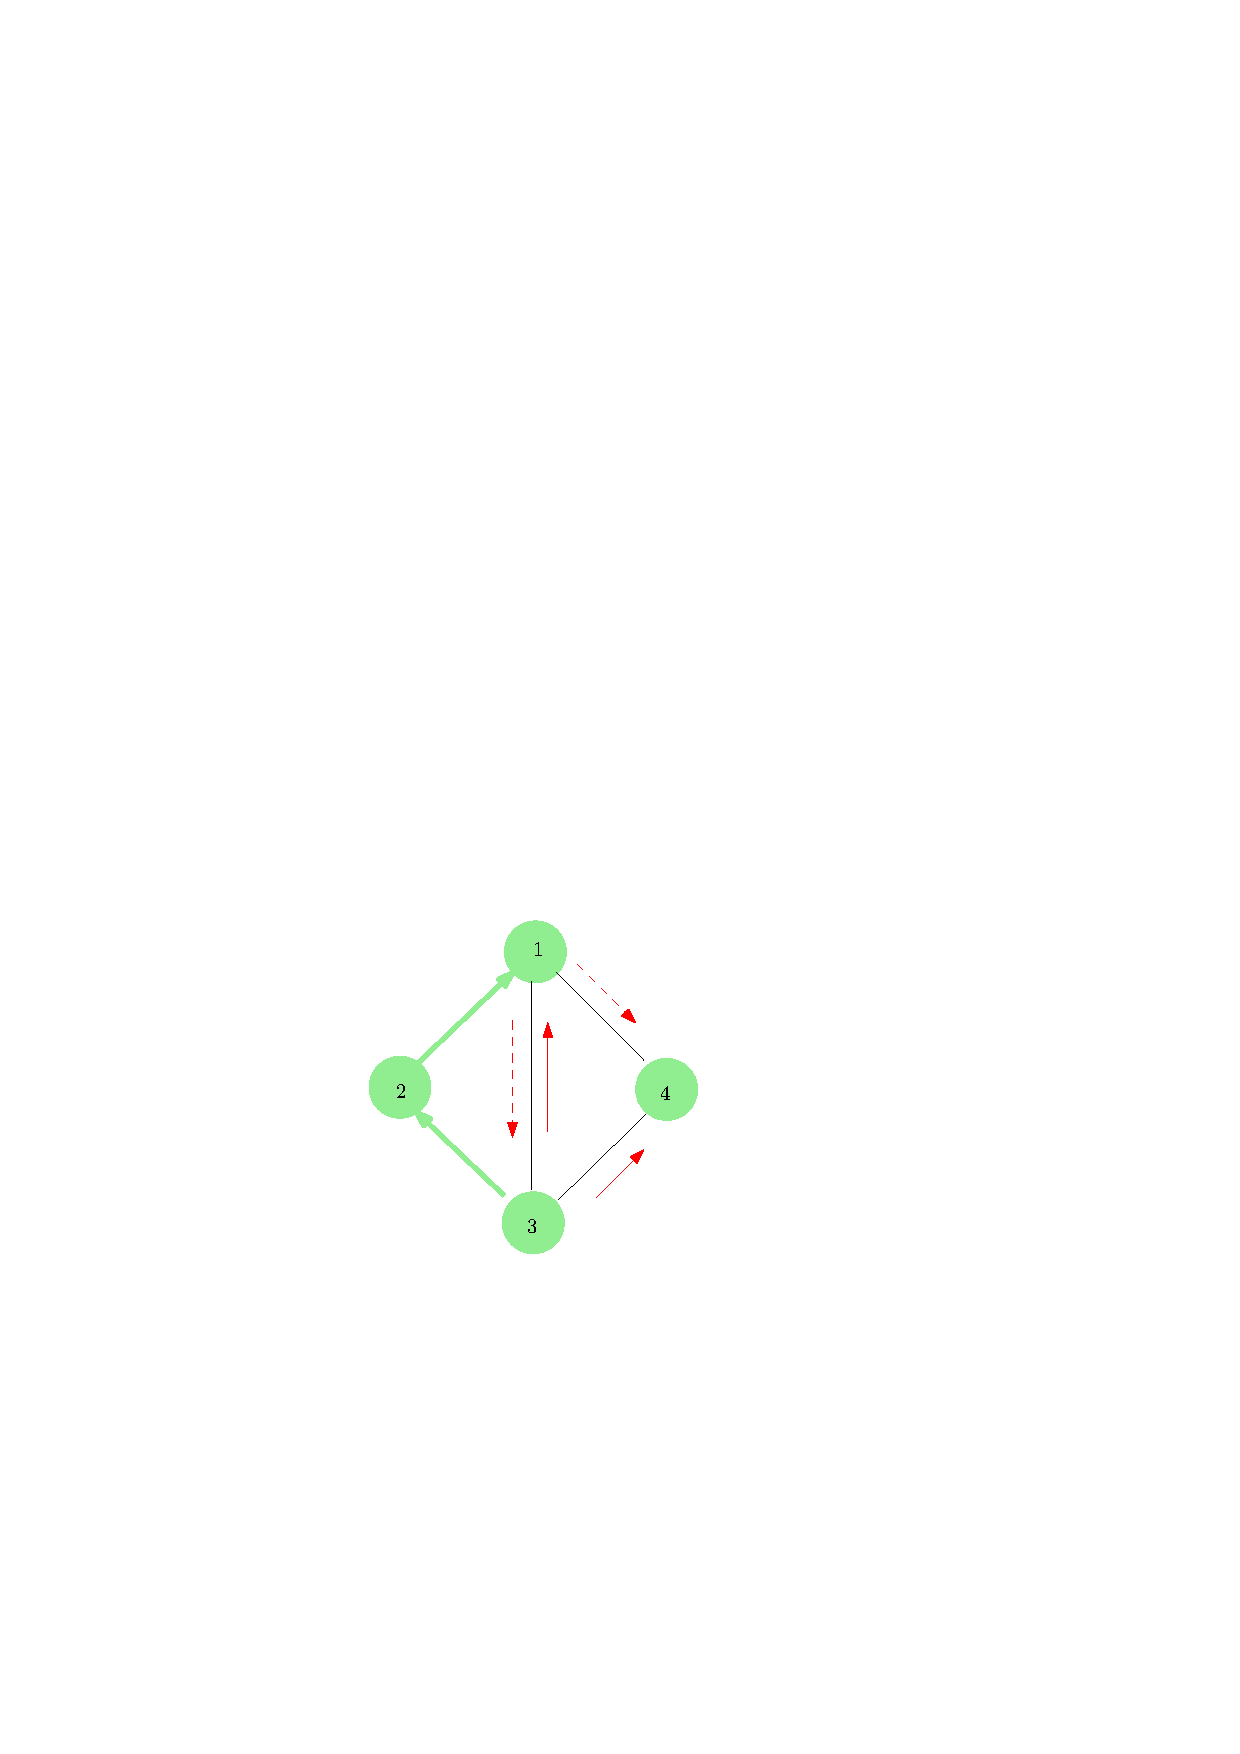
\includegraphics[width=0.32\textwidth]{chapters/background/images/echo/async/notext_f0_3.pdf}}
    \subcaptionbox{Round Four}{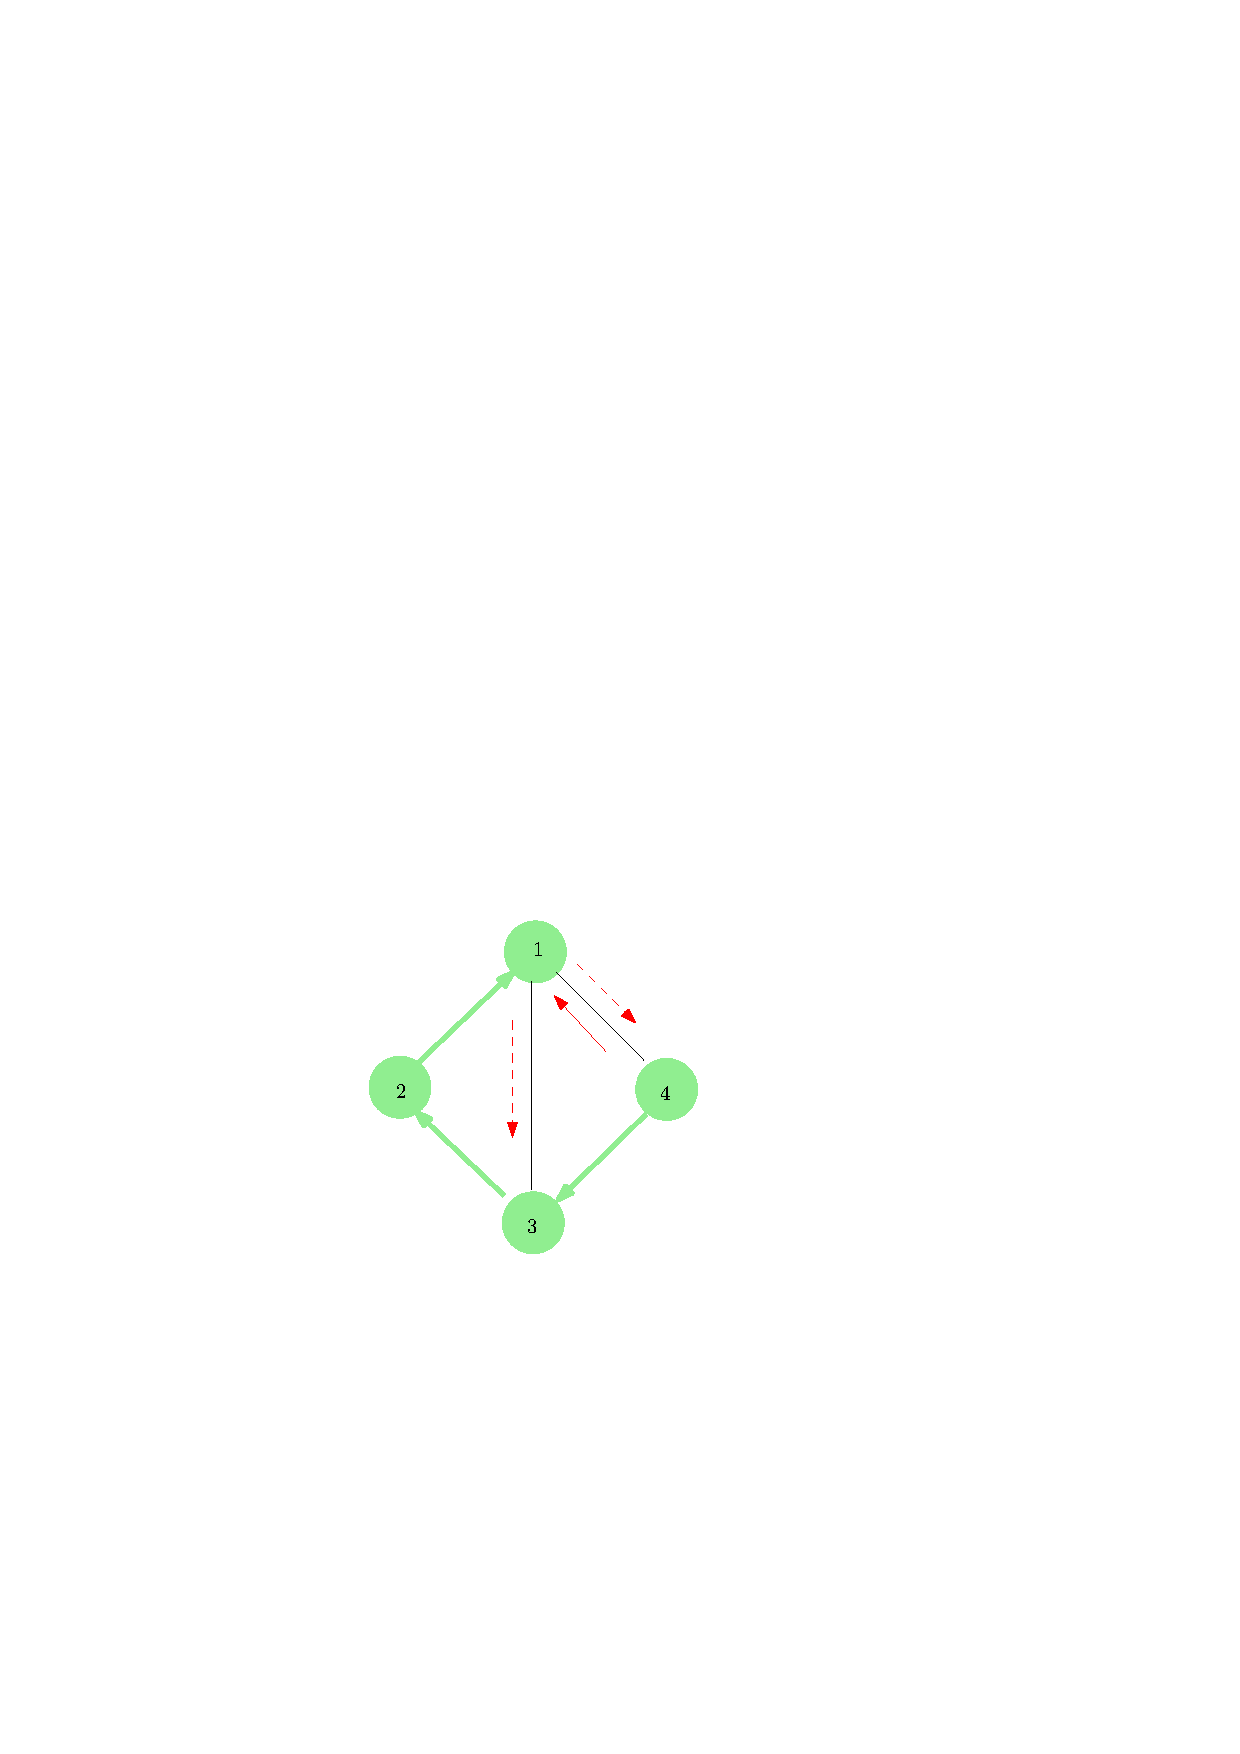
\includegraphics[width=0.32\textwidth]{chapters/background/images/echo/async/notext_f0_4.pdf}}
    \subcaptionbox{Round Five}{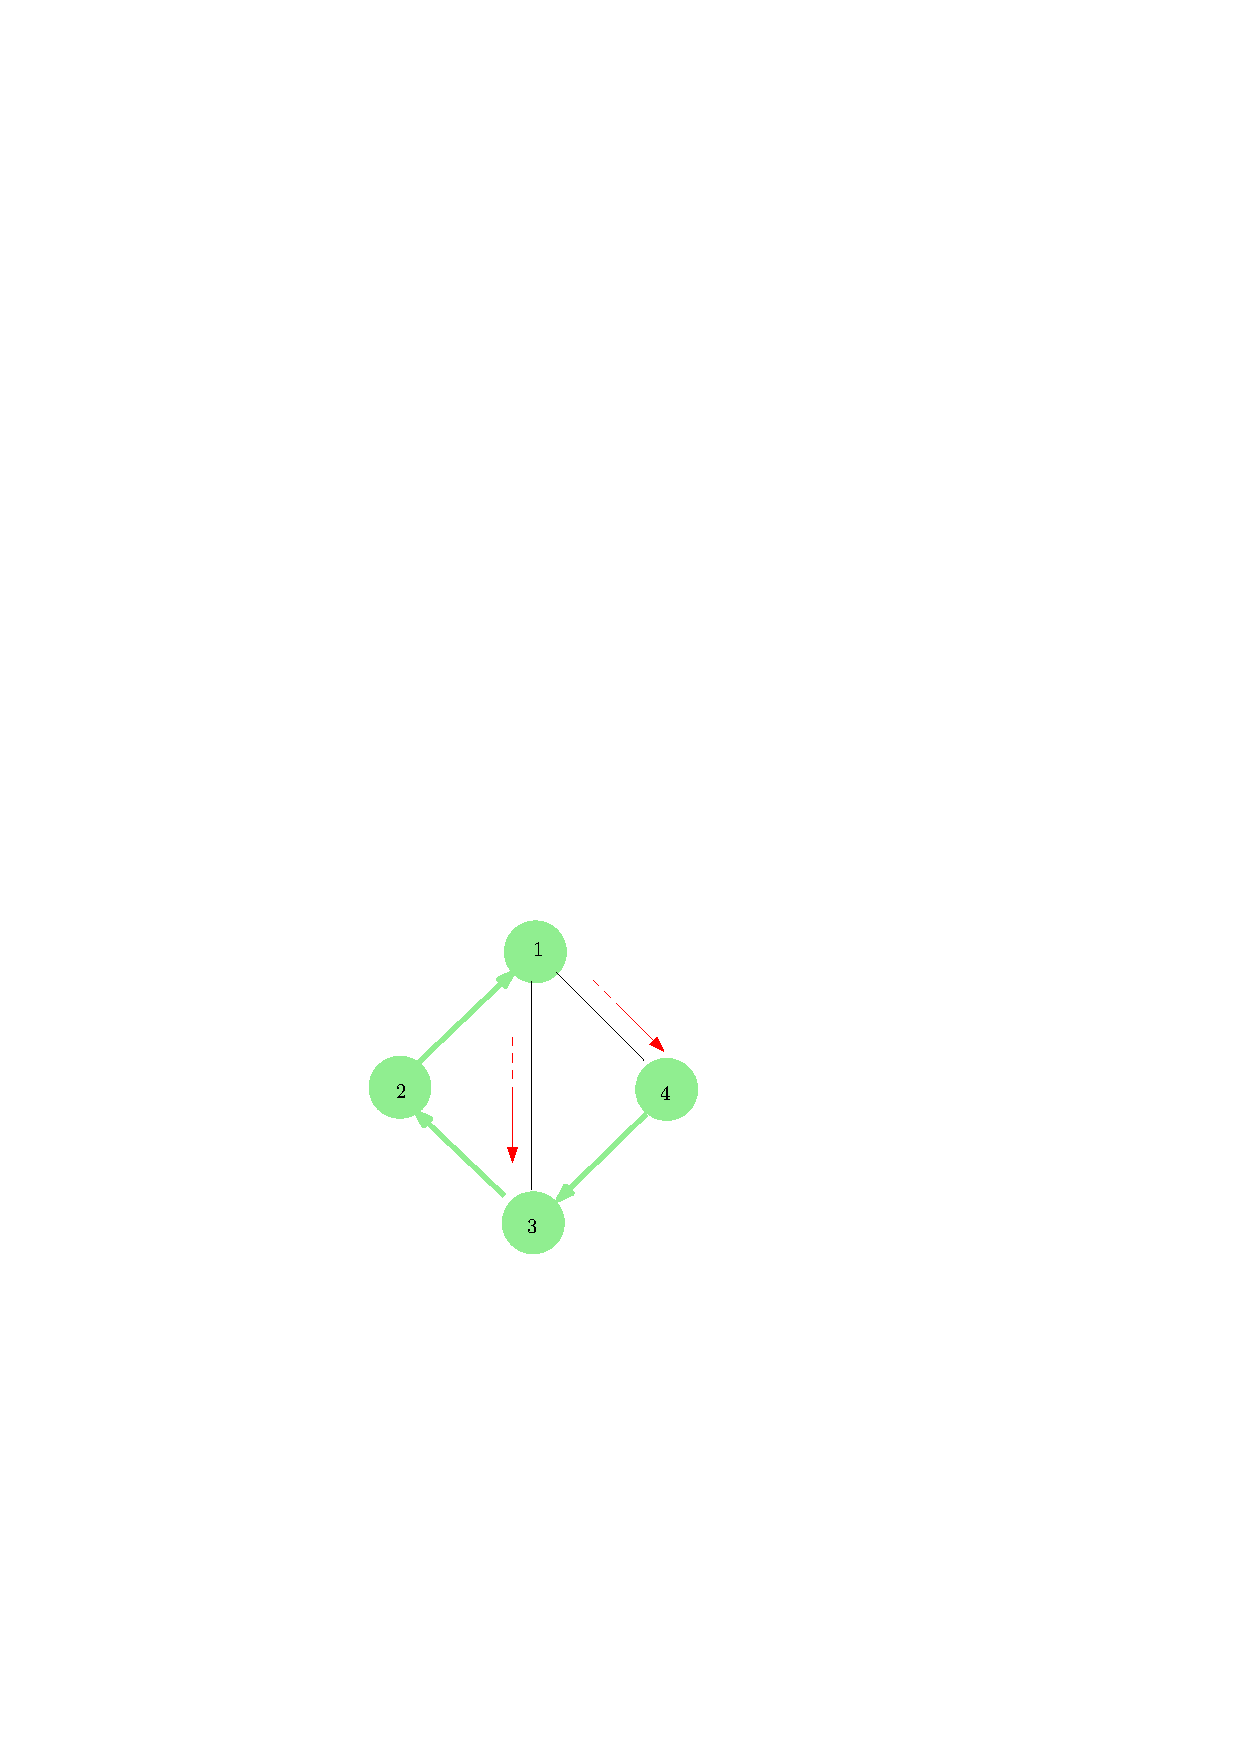
\includegraphics[width=0.32\textwidth]{chapters/background/images/echo/async/notext_f0_5.pdf}}
    \subcaptionbox{Round Six}{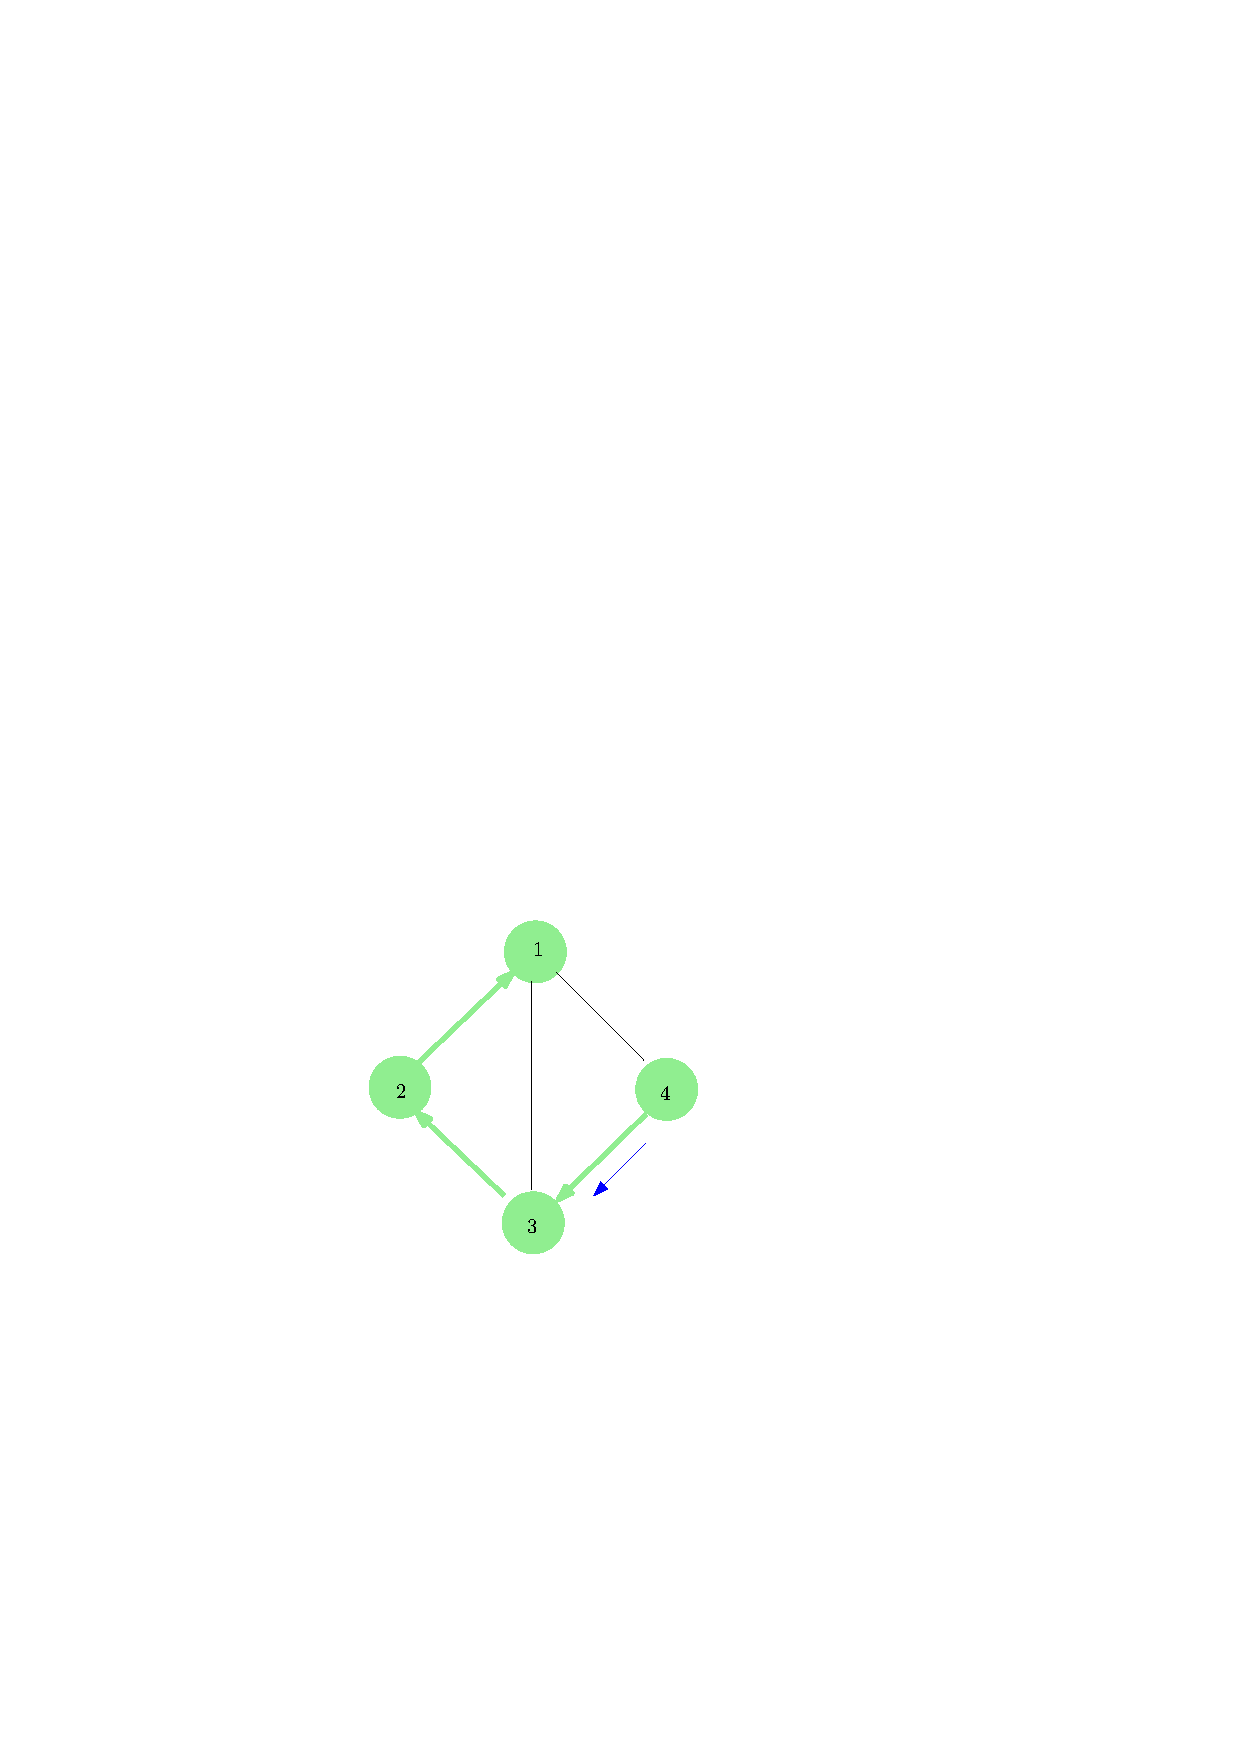
\includegraphics[width=0.32\textwidth]{chapters/background/images/echo/async/notext_f0_6.pdf}}
    \subcaptionbox{Round Seven}{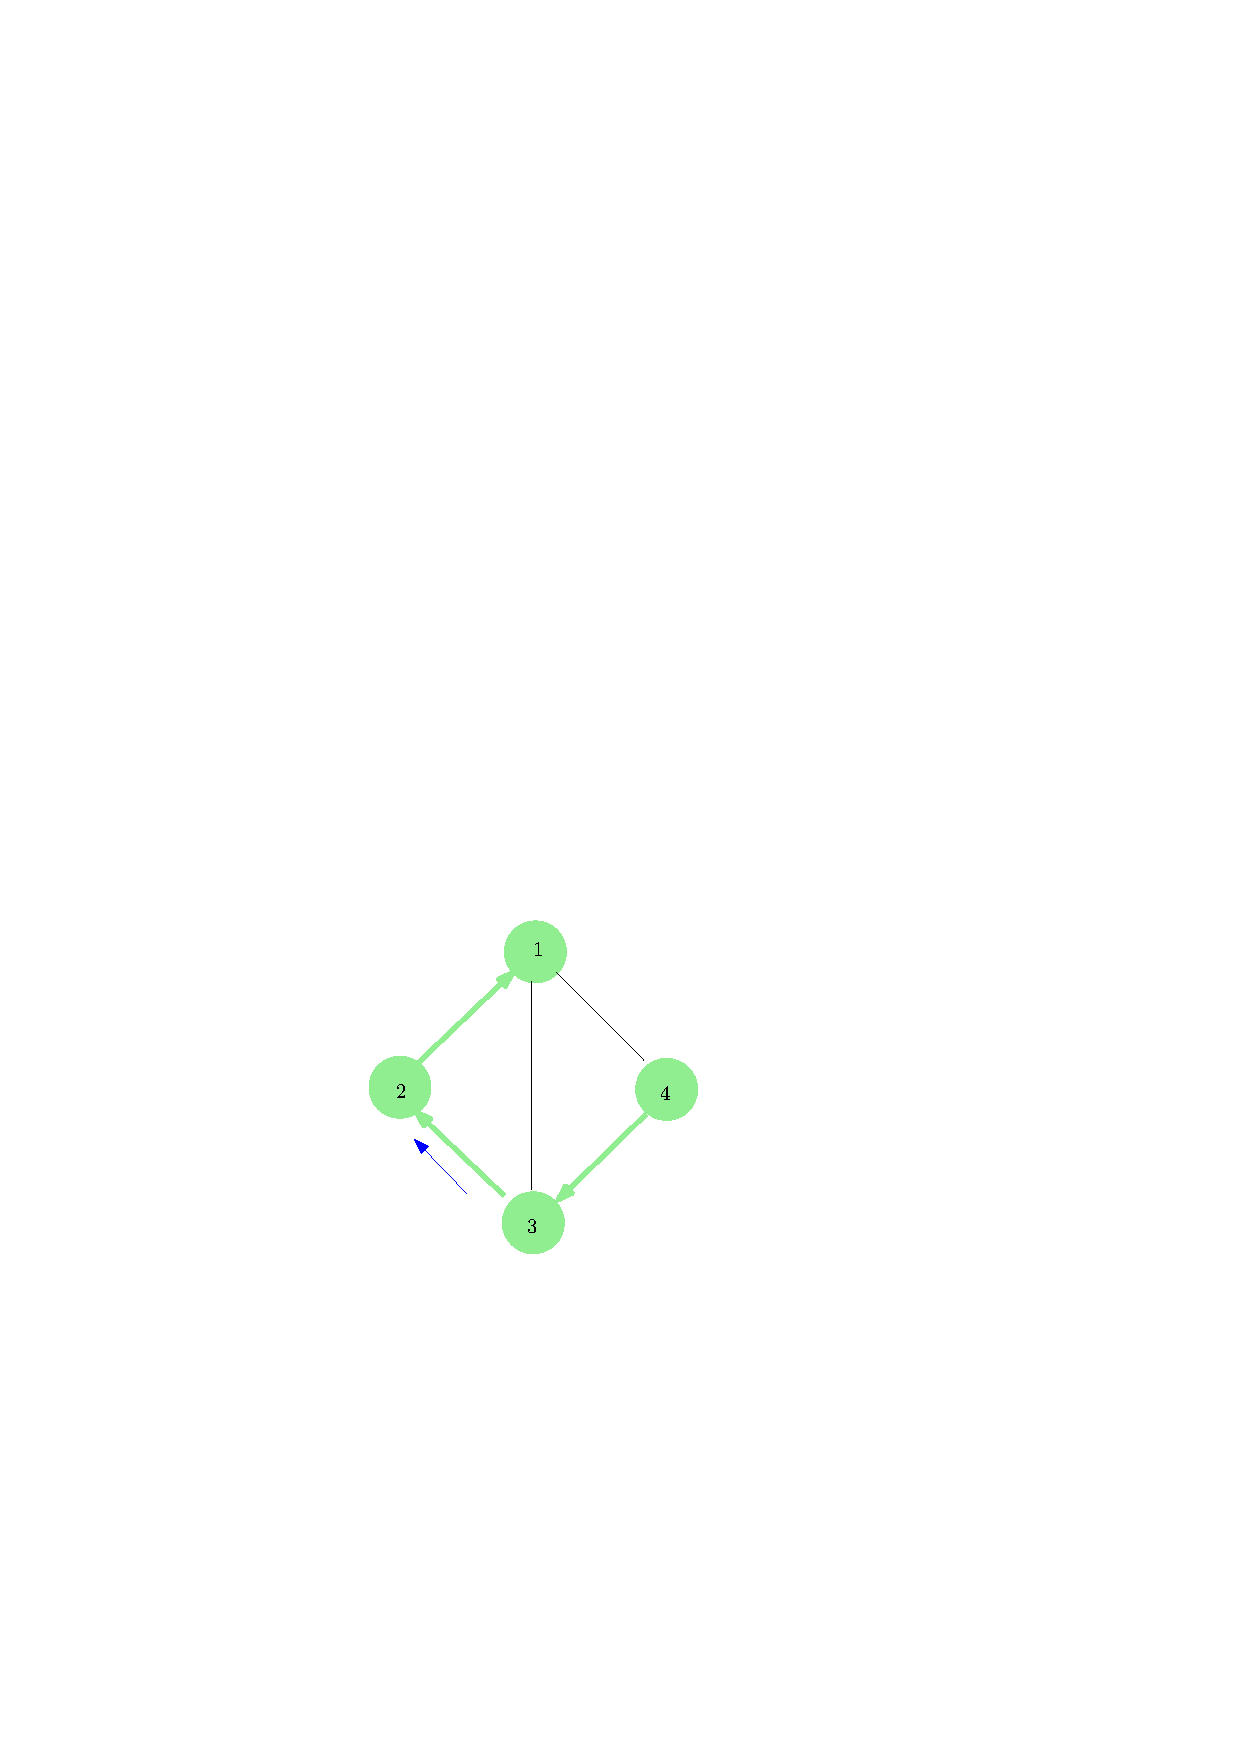
\includegraphics[width=0.32\textwidth]{chapters/background/images/echo/async/notext_f0_7.pdf}}
    \subcaptionbox{Round Eight}{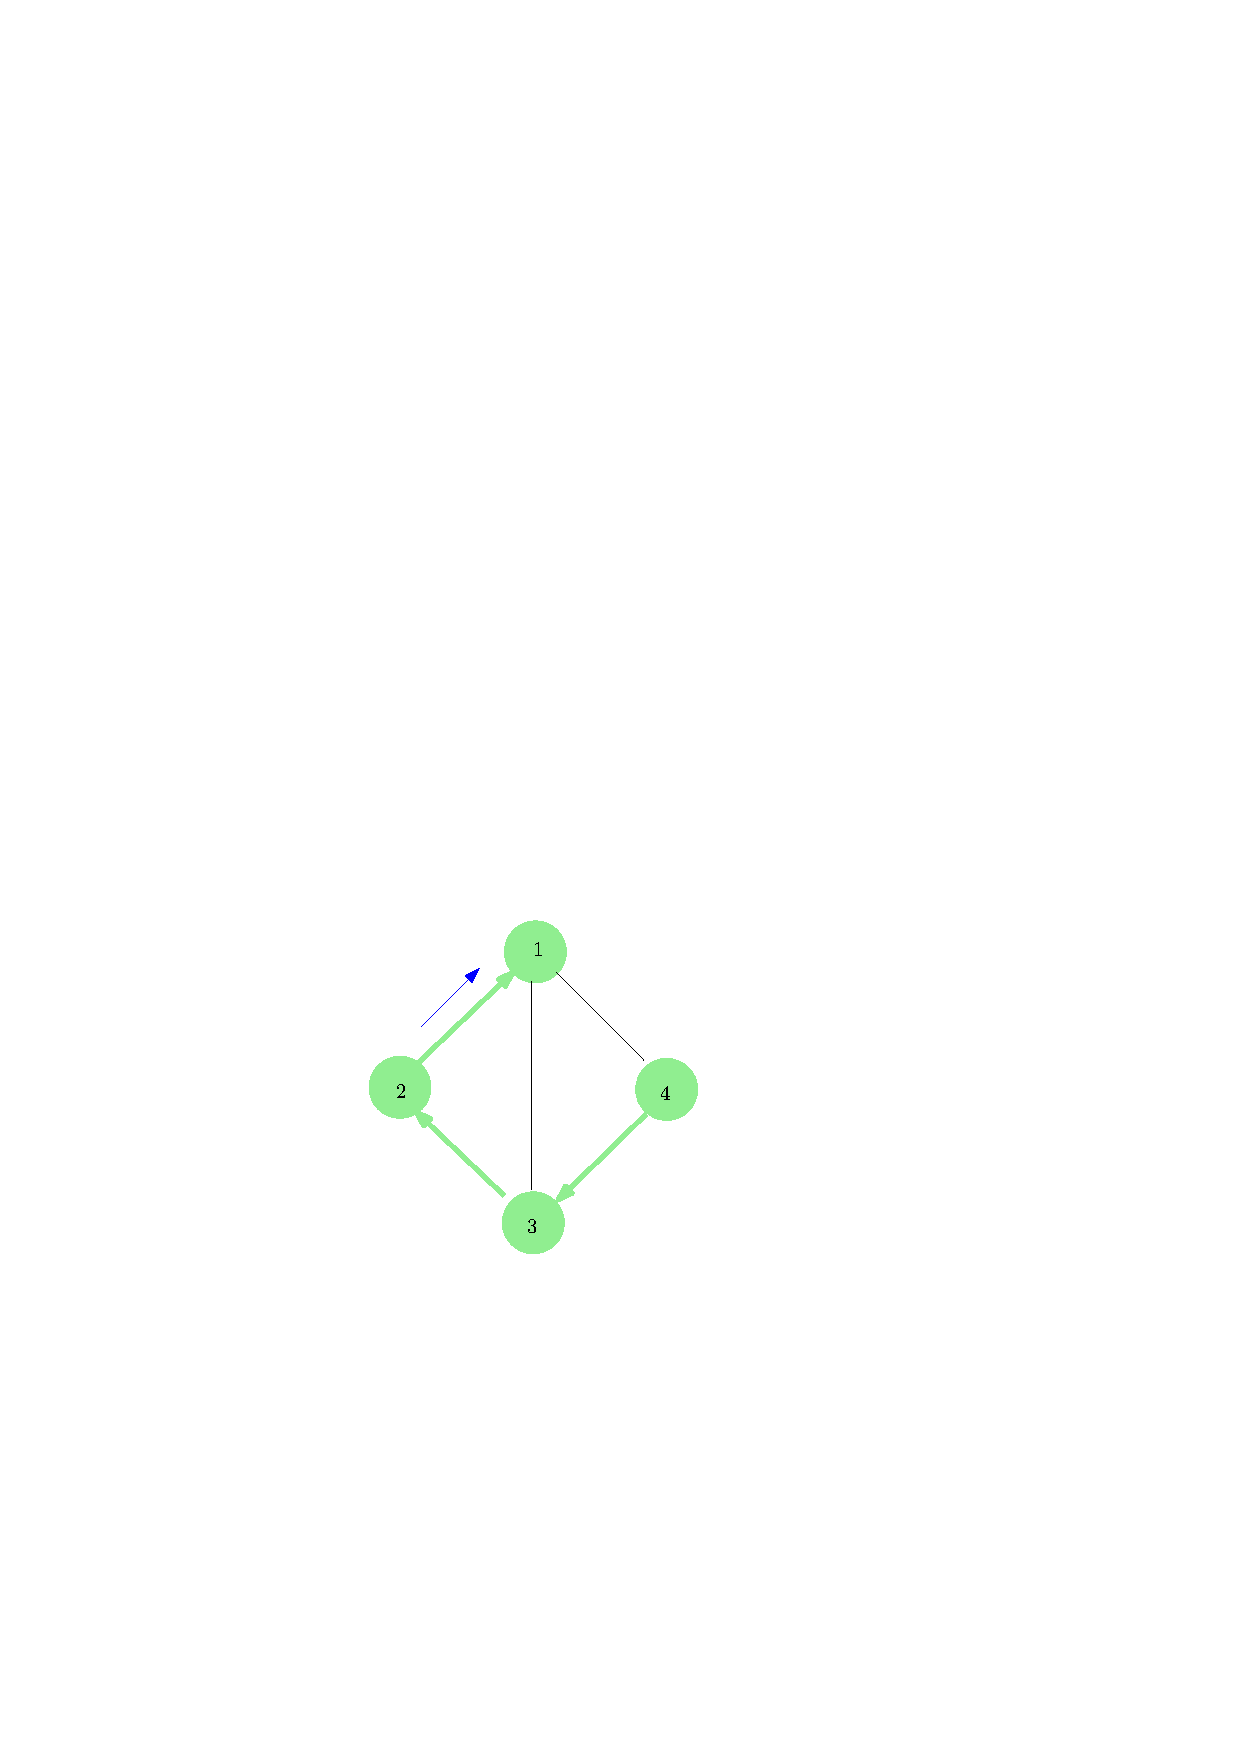
\includegraphics[width=0.32\textwidth]{chapters/background/images/echo/async/notext_f0_8.pdf}}
    \caption[Progression of the asynchronous \textsf{echo} algorithm]{Progression of the asynchronous \textsf{echo} algorithm, starting from round zero before any messages are sent.  Arrows in red mean broadcast messages, while arrows in blue mean convergecast messages.  Despite node 1 being the initiator node, node 4 considers node 3 to be its parent because it first receives a broadcast message from node 3.}
    \label{fig:back:echoasync}
\end{figure}

In the synchronous case, all messages sent out are received simultaneously, and all nodes proceed through their rounds together.  In the asynchronous case, however, messages may arrive at arbitrary times, and nodes proceed through their rounds entirely independently of one another.  The round numbers in the figure mark the point where at least one message has been received by a node.  The nodes react to messages as they arrive, and might do nothing for a time while other nodes are working if no new messages arrive during that time.  Under the asynchronous model, depending on communications topology and speeds, it is possible for the first broadcast message to reach a process to have followed a less direct route from the initiator than otherwise might be possible.  Exactly this is seen in \cref{fig:back:echoasync:3}, where node 4 first receives a message from node 3 (and thus marks node 3 as its parent), despite a direct connection to the initiator, node 1.
\section{\label{sec:back:cml}\glsfmtlong{cml-glossary}}

While parallelism is often the best (perhaps only) way to achieve improvements in execution time for different algorithms once an efficient sequential implementation has been created, it is a notoriously challenging affair \cite{Shun2017}.  When working at the level of directly manipulating threads, such as using the pthreads found in POSIX-compliant operating systems, programmers are exposed to a high level of risk of inadvertently introducing concurrency bugs, such as data races, deadlocks and livelocks.  A panoply of approaches to overcoming this challenge, both theoretical and practical, have been proposed and developed over the years, with varying degrees of success, \eg{} \cite{Boyapati2002,Bocq2012,Seinstra2004}.  Many, perhaps most, large-scale programming languages that use a runtime include some form of parallelism simplification within their standard libraries, \eg{} the Executor system in Java \cite[Ch. 4]{Fernandez2012}, and Swift \& Objective-C's Grand Central Dispatch \cite{Maskrey2018}.

Most simplifications fairly directly target either data-parallelism by simultaneously applying the same operation over multiple elements in arrays, \eg{} SIMD instructions in CPUs \cite{Hughes2015}; or task-parallelism by making provisions for the fork-join model \cite{McCool2012}.  These simplifications can be very useful, but not all instances of parallelism fit neatly into their models.  Algorithms that are well-modelled by the \Gls{csp} and \Gls{actor} models, such as those explicitly centred around concepts of message passing, are not necessarily easy to express using either SIMD or fork-join instructions.

\Gls{cml} \cite{Reppy1991,Panangaden1997} is an approach to concurrent programming originally developed by John Reppy (based on his earlier `Pegasus Meta-Language' \cite{Reppy1988}).  \Gls{cml} was created to provide a framework for creating concurrent programs with synchronous communications on single-core machines,\footnote{In fact, the original implementation \emph{relied} on the fact that the processor was single-core under-the-covers.} and was later extended to permit parallelism \cite{Reppy2009a}.  It was created originally as a library in Standard ML of New Jersey (where ML refers to the earlier programming language \textit{Meta Language}), whence the ML part of the name, but its concepts have subsequently appeared elsewhere.  The basic concept of communicating via channels has experienced a renaissance in recent years, likely due at least in part to its inclusion as a core feature of Go \cite{Meyerson2014}, but \gls{cml} has a more advanced system that Go (at the time of writing) does not fully support.

\Gls{cml} is designed to avoid many of the problems with concurrency that arise in traditional sequential programming, where the use of locks, mutexes and semaphores etc. are frequently required, and often lead to the potential introduction of problems such live-/deadlocks, data races and extreme resource contention.  This is achieved by changing the approach to concurrent programming to one of logically separate, internally sequential processing elements that share data as required by `passing messages'\footnote{This is the logical concept, but there is not strictly any specific required software implementation.} between themselves.  In \gls{cml}, these logical processing elements are referred to as threads, and they exchange messages over channels \emph{synchronously} (called \emph{rendezvous}), \ie{} there is a temporal overlap between one thread offering to send, and another to receive, over the same channel, and the first to offer blocks until the second makes its offer.  When two processes are offering appropriately on either side of an exchange, rendezvous takes place.

Reppy describes a concurrent program as one that supports multiple sequential sub-programs conceptually executing in parallel separately, but interacting through shared resources to achieve a common goal.  \Gls{cml} is concerned with the scenario where said interactions are explicit, and in order to facilitate that \enquote{\gls{cml} takes the unique approach of supporting \emph{higher-order concurrent programming}} (emphasis Reppy's), whereby communication and synchronisation are made into first-class members of the language, similar to how functional programming languages made functions into first-class members of themselves \cite[Preface]{Reppy2007}.

\begin{anfxerror}{Expand this?}
Describe more of how \gls{cml} works?  Is there not something in the gcol chapter that can be shifted into here, at least?
\end{anfxerror}
\section{\label{sec:back:mc}\Glsfmtname{mc}/\glsfmtname{ps}}

\emph{\Gls{mc}}, also known as \emph{\gls{ps}} (the two terms are generally used interchangeably), is a bio-inspired model of computing created by Gheorghe Păun in the late 1990s \cite{tPaun98a,Paun2000}.  It was originally conceived of by considering the process of chemical reactions and exchanges that occur inside living biological cells and the membranes within, and regarding this process as a form of computation.  \Gls{mc} was identified in 2016 by the National Research Council of Canada as \textcquote[][p. 17]{Wiseman2016}{a rigorous and comprehensive framework that provides a parallel distributed framework with flexible evolution rules.}

\citeauthor{Paun2002} describes \gls{mc} as:
\blockcquote[][p.~VII]{Paun2002}{Membrane computing is a branch of natural computing which abstracts from the structure and the functioning of living cells. In the basic model, the membrane systems -- also called P systems -- are distributed parallel computing devices, processing multisets of objects, synchronously, in the compartments delimited by a membrane structure. The objects, which correspond to chemicals evolving in the compartments of a cell, can also pass through membranes. The membranes form a hierarchical structure --- they can be dissolved, divided, created, and their permeability can be modified. A sequence of transitions between configurations of a system forms a computation. The result of a halting computation is the number of objects present at the end of the computation in a specified membrane, called the output membrane. The objects can also have a structure of their own that can be described by strings over a given alphabet of basic molecules - then the result of a computation is a set of strings.}

\begin{anfxerror}{P systems Diagram?}
Include a copy of the membrane layout diagram from Paun?
\end{anfxerror}

\Gls{ps} works analogously to a typical modern electronic computer, in that the system stores data and processes \& updates those data based on a predefined program, with a view to arriving at a computable answer based on the starting state and any inputs to the system \cite{Paun2002,Paun2010b}.  In classical \gls{ps}, the data are multisets of symbols, representing various chemicals and their quantities.  These are found inside one or more \emph{cells},\footnote{Loosely based on real biological cells.} which (to a certain extent at least) form a hybrid between main memory and the processing units of a computer.  The instructions of the program itself are provided by \emph{rules}, which specify transformations of objects and interactions with the surrounding environment and other membranes or cells.

There are now, broadly, three main families of \gls{ps} variants:  \gls{clps} \cite{Paun2001,Paun2002}, \gls{tlps} \cite{tMaPaPaRo01a,Martin-Vide2003} and \gls{snps} \cite{Ionescu2006}.\footnote{Several other variants have been created, but most are used infrequently, if ever.  Most recent work in \gls{mc} has focused on sub-variants of \gls{clps}, \gls{tlps}, \gls{snps} and \gls{cps}.}  \Gls{clps} is the direct descendant of the original classical \gls{ps}, and sees objects compartmented into \emph{membranes}, which are arranged in a graphical tree structure with the outermost \emph{skin} membrane -- which separates the cell from its environment -- as the root of the tree.  In most variants, objects can evolve inside a membrane, but also be communicated between membranes (and the environment).  Furthermore, membranes can \emph{divide} or \emph{dissolve} themselves, and may have one or more special properties, such as \emph{polarization} \cite{Paun1999a}.

On the other hand, \gls{tlps} and \gls{snps} both arrange their computing compartments -- named \emph{cells} or \emph{neurons}, respectively -- as nodes in arbitrary digraphs, with the edges between them representing connecting channels or synapses.  Whereas \gls{clps} emphasises the evolution of multisets of objects inside membranes of a given cell, \gls{tlps} and \gls{snps} emphasise communication between separate cells/neurons, and might not include any capacity for internal evolution inside cells.  If new objects are required, they are imported via communication with the environment, which possesses an unlimited number of all objects but has no rules of its own.

While \gls{tlps} have arbitrary alphabets, only one object is used in \gls{snps}, the \emph{spike}.  This means that \gls{tlps} are frequently much like \gls{clps} in that they have custom objects for each purpose, with the key difference (usually) being in the arrangement of the compartments/membranes/cells relative to each other and the choice between the two motivated primarily by which one better fits the computation to be modelled.

Conversely, \gls{snps} represent everything through the use of differing quantities of the spike, kept in different neurons.  This means that it can be more complex to model certain problems, but also arguably means that \gls{snps} are, \textit{prima facie}, closer to Lambda Calculus \cite{Barendregt1984} and Church Numerals (see \eg{} \cite{Koopman2014,Hinze2005}), as well as Register Machines (see \eg{} \cite{Korec1996}) (and indeed Register Machines have been simulated with \gls{snps} \cite{Pan2010}).  All three main types of \gls{ps}, in some form, have been proven Turing-universal though \cite{Bernardini2005,Chen2008,Freund2005}, so all three should be capable of expressing the same computations in different forms.  Furthermore, because \gls{snps} can be easily represented numerically, they lend themselves well to vector/matrix representations \cite{Zeng2010,Martinez-del-Amor2021,Gheorghe2021,Hu2016}.  This means that, potentially, \gls{snps} implementations can take advantage of high-performance techniques such as directly using \gls{blas} \& \gls{lapack} and/or \glspl{gpu} \cite{Aboy2019}.

Arguably, the most noteworthy and important aspects of \gls{ps} models are that:
\begin{inparaenum}[(i)]
\item They have no space limit.  That is, they contain an unbounded number of cells, objects and membranes;
\item Usually, across all cells and membranes, all rules that can be applied are applied, as many times as possible given the current number of objects available.
\end{inparaenum}
These two features mean that \gls{ps} have unbounded space and processing capacity, which can be used to solve traditionally computationally difficult problems relatively quickly \cite{Sosik2003,Jimenez2003,Paun1999a,Henderson2020}.  Most of these solutions, however, rely on trading time complexity for space complexity.  While this works in the theoretical framework, electronic simulations of the systems do not have access to unlimited instantaneous memory space, meaning many of the fast solutions are impractical with current real-world computers, \eg{} \cite{Cooper2019,Cooper2019a} \fxnote[inline]{[refs]} (see further \vref{sec:psystemsuses}).

\citeauthor{Valencia-Cabrera2019} said of this:
\blockcquote[][p.~213]{Valencia-Cabrera2019}{We do not know if we will have those machines able to solve NP-complete problems in polynomial time, in many cases even linear time, but \textins{that does} not necessarily mean we will have to wait until that moment in biochemical technology to find some relevant use of P systems. As Babbage kept working on his ideas, not simply waiting until the precise moment when Turing, Von Neumann, and their contemporaries witnessed the first electronic computers based on similar principles, membrane computing must keep moving, finding new ways to provide a step further.}

Nevertheless, modelling a problem in \gls{mc} can lead to new insights or improved formulations of solutions, as occurs in \cref{chap:nmp}.  For example, in \cite{GimelFarb2013a} (building on \cite{Gimelfarb2011}) \citeauthor{GimelFarb2013a} describe how formulating Symmetric Dynamic Programming \gls{sm} in terms of \gls{ps} led to finding a bug in the implementation, \textcquote[][p.~24]{GimelFarb2013a}{but also (and what is much more important) refactor this algorithm, based on our cell structure.  The result is a more robust and flexible version, which allows us to fine tune its parameters and enhance its capabilities, without rewriting it from scratch.}  Furthermore, as reported in \cite{Nicolescu2014b}, this exercise led directly to the creation of a new \gls{sm} algorithm, Concurrent Propagation \cite{Gimelfarb2012}.  \citeauthor{Pang2018} \cite{Pang2018} also claim significant benefits from modelling certain problems in a novel variant of \gls{enps} \cite{Pavel2010}, but it is unclear how much of the stated benefit compared to their baseline implementation arises instead from the use of a \gls{gpu}.

\subsection{Objects, Rules and Steps}
All known \gls{ps} types fundamentally operate on a similar basis:  One or more sets of rules -- \emph{\gls{ruleset}} -- are defined, describing how the \emph{objects} present in the system's compartments change at each \emph{step}.  As mentioned above, the objects are usually multisets of arbitrary symbolic \emph{atoms}, with the exceptions of \gls{snps} which uses the spike as its only symbol, and Numerical \gls{ps}, which uses ordinary numbers in place of atoms.  Certain systems may introduce other object types as required.

\Gls{ps} types normally operate synchronously and assume the presence of a global clock.  At each clock ``tick'', every compartment compares its extant objects and its \emph{evolution rules}, determines which rules are applicable given the current objects, and then deletes the objects used in the rules, replacing them with new ones as the rules dictate.  This process comprises a step.  The progressive execution of the system's rules over multiple steps is referred to as the system's evolution.

All \gls{ps} evolve, and therefore all types have evolution rules (though they may not be referred to as such).  Other types of rules are possible, including: \emph{dissolution} and \emph{division} rules in \gls{clps} and \gls{tlps}, where membranes either dissolve and release their objects into the their parent membrane, or replicate themselves (essentially performing mitosis) and distribute their contents among the new membranes; \emph{forgetting} rules in \gls{snps} whereby one or more copies of the spike are removed from a given neuron; or, splicing rules in Splicing \Gls{ps}\footnote{Particularly notable for working over strings of an alphabet, instead of multisets.} \cite[Ch.~8]{Paun2010b}.

All rules use the same basic model.  At the start of a step, they check if the necessary pre-conditions for the rule are met.  If they are, then any changes to the state of the system specified by the rule occur.  It is common for rules to remove or delete some objects in the relevant compartment, and instantiate new ones.  It is typically assumed that all objects are deleted or created instantaneously at the last moment of the rules' execution.

Generally, rules are specified in the form \textsc{\gls{lhs}} \(\rightarrow\) \textsc{\gls{rhs}}, where objects to be removed (the presence of which are therefore a precondition) are written in the \gls{lhs} and the objects to be created are written in the \gls{rhs}.  Unless otherwise specified, it is typically assumed that all rules which can be applied at a given step are applied.

\subsubsection{Weak Priority Order}

Many, perhaps most, types of \gls{ps} \glspl{ruleset} use a \emph{weak-priority} ordering.  This means that some rules will be tested for applicability ahead of others, on some priority basis, but earlier applicable rules only prevent later applicable rules from being applied if there is a conflict between the two.  The most common way that this conflict can arise is by two rules trying to use the same pre-existing object in the compartment.

Generally speaking, an individual rule will select for use one or more copies of one or more objects the multiset.  At the end of the rule's application, these objects are deleted and replaced with any new ones the rule specifies.  Since the rule will delete the chosen objects, it would not make sense for another rule to be able also to use and then delete the same objects.  Therefore, the first rule to select (or take hold of or seize \etc{}) a given object prevents any other rule from using it too, and thus the first rule has priority over later rules.

The typical method of defining rules' priority is to use \emph{top-down} ordering.  This simply means that the rules presented first in a \gls{ruleset} have priority over those rules presented further down.  The basic process to determine which rules to apply is therefore a sequential one.  Starting with the first rule, and proceeding with each successive rule in turn, test if the rule is applicable at all.  If it is, set it to be applied during the step as many times as possible depending on the rule, the objects present, and the run-time mode (see \eg{} \cref{sec:cps:applicationmodes} for a discussion of this in relation to \gls{cps}).

Any objects now set to be deleted by a previous rule are then unavailable to a later rule, but if there are sufficient remaining objects for that rule to apply, it still may, giving a \emph{weak} priority to the earlier rules.  The application of an earlier rule does not guarantee that a later rule will not apply, but the earlier rule takes precedence in the case of a conflict.  Furthermore, some \gls{ps} variants, \gls{cps} included, use states on their compartments (or the system as a whole).  In this case, rules will usually state a necessary starting state, and an ending state to which the rule transitions the system.  The first such rule to apply dictates the ending state of the compartment (or system) at the end of the step.  Rules with a lower priority may then only be applied if they have the same requisite ending state.

%%%%%%%%%%%%%%%%%%%%%%%%%%%%%%%%%%

\subsection{Computer Representations and Simulations of \glsfmtname{ps}}

\subsubsection{\Adhoc{} and General Simulations}
There are arguably two main approaches to simulating \gls{ps}:
\begin{inparaenum}[a)]
\item ``\Adhoc{}'' simulations, where a separate program is written specifically for a given type of problem and its \gls{ps} solution; and
\item ``General'' simulations, where a separate simulation engine capable of simulating one or more types of \glspl{ps} is created independent of a given problem, and is supplied problem-specific configurations.  The engine uses the configuration to initialise the simulated system, and works through the problem from there.
\end{inparaenum}

The main advantage of the \adhoc{} style is the ability to adjust and optimise the simulation's implementation to suit the \gls{ps} variant used, and the problem at hand.  In general, \adhoc{} simulations would be expected to require less resources to find the answer, \eg{} running faster and/or using less memory.  The major disadvantage of the \adhoc{} approach is that a new simulation must be developed for each problem studied, requiring more time and greater levels of technical skill while reducing flexibility.  The main advantages of the general approach are greater flexibility from the produced program -- \ie{} it can simulate more problems -- and a broadening of the people who can experiment with different \gls{ps} variants and problems to those with lower levels of programming expertise.

General simulations permit specialisation and a division of labour, meaning one person can look into new \gls{ps} variants and problems to apply them to, while another person focuses on developing and improving the simulation engine itself.  This is a clear upside, but there is equally a downside: lacking problem-specific knowledge, the general simulations usually do not perform all potential optimisations, meaning that there could be unavoidable upper bounds on the efficiency of a simulation, no matter the specific problem at hand.  Furthermore, general simulations must run inside another program, whereas \adhoc{} simulations can be created as independent, native executables.

Traditionally, this has been an `either/or' problem, where one can take either a wholly \adhoc{} approach or a wholly generalist approach.  \citeauthor{Perez-Hurtado2019} more recently introduced a \gls{ps} ``compiler'' \texttt{pcc} \cite{Perez-Hurtado2019}, which can produce a standalone native executable from a non-programmatic specification of a particular \glspl{ps} --- thus providing a third, middle-ground option.  They say of this compiler: \textquote{the goal of \textins{\texttt{pcc}} is twofold: On the one hand, it purports to be a good assistant for researchers while verifying their designs, even working with experimental models. On the other hand, it provides optimized simulators for real applications, such as robotics or simulation of biological phenomena.}  It was not used in this dissertation, as \texttt{pcc} did not support \gls{cps} at the relevant time, but the idea holds great promise for the future.

%%%%%%%%%%%%%%%%%%%%%%%%

\subsubsection{\label{sec:back:simulators}\Glsfmtname{ps} Simulators}

\citeauthor{Valencia-Cabrera2019} provide a summary of the development of simulators for \Gls{ps} since the field's inception in the late 1990s \cite{Valencia-Cabrera2019}.\footnote{The authors also provide a timeline of practical works in \gls{ps} at \url{https://github.com/RGNC/plingua}.  Some of the software described in this \lcnamecref{sec:back:simulators} is available at \url{http://ppage.psystems.eu/index.php/Software/}.}  Unsurprisingly, most early simulators were \adhoc{} and created for a specific purpose, focusing on one problem domain and simulating one \gls{ps} variant.  Many were intended for formal verification of models as much as they were for practical use \cite{Gutierrez-Naranjo2007}.  These early simulations were written in a wide variety of programming languages, including (comparatively) lesser-used languages such as Haskell, Prolog and LISP.  Notably, \citeauthor{Ciobanu2004} created a simulator specifically for distributed computing, using C++ and \gls{mpi} \cite{Ciobanu2004}.

As the number of \gls{ps} variants defined, and simulations to experiment with them, expanded greatly, it began to make more sense to create general simulators which did not require detailed customisation for every experiment.  A handful of these multi-purpose simulators began to appear, including (among others): PSim \cite{Bianco2007,Bianco2007a}; a transpiler from Systems Biology Markup Language (SBML) to C Language Integrated Production System (CLIPS) \cite{NepomucenoChamorro2005};  and a web-based simulator which also made use of CLIPS \cite{Bonchis2005}.  Of particular interest from this period is \cite{Acampora2007}, which specifically targeted the creation of a paralel and distributed multi-agent system, to take advantage of the concurrency inherent in most \gls{ps} variants and models.

While these simulators were a clear step to re-usability, they still largely targeted only a specific \gls{ps} variant or sub-variant.  There was another issue in that there was no standard for representing an individual \glspl{ps}.  Simulators generally either used their own custom specification system, such as a special-purpose XML schema, or attempted to make use of a representation created for another purpose, such as SBML.  To address these two shortcomings of the existing systems, researchers at the Universidad de Sevilla (University of Seville) in Spain created \gls{plingua}\footnote{\url{http://www.p-lingua.org/wiki/index.php/Main_Page}, \url{https://github.com/RGNC/plingua}} \cite{Diaz-Pernil2008a,Garcia-Quismondo2010} and \gls{mecosim}\footnote{\url{http://www.p-lingua.org/mecosim/}} \cite{Perez-Hurtado2010}.

\Gls{plingua} is a declarative markup language, used to specify specific systems and their initial configurations.  Arguably, it has become the dominant specification language of the computerised \gls{ps} world.  Crucially, \gls{plingua} also allows for the specification of new \gls{ps} variants and extensions to existing ones, giving it a much greater potential flexibility.  It is primarily built around the Java library PLinguaCore, which provides functionality to translate between various representations of \gls{ps} specifications.  One of the simulators to make heavy use of \gls{plingua} is \gls{mecosim}.

\Gls{mecosim} is a Java-based general-purpose \gls{mc} simulator.  It uses \gls{plingua} and spreadsheets to define the evolution of a given \gls{ps} type, as well as the problem to be solved --- both the rules and starting state of the system.  The particular strengths of \gls{mecosim} are that, once a particular type of \glspl{ps} has been defined it is completely re-usable, and the simulator permits rapid experimentation with different designs without any programming.  Sadly, however, it appears that both \gls{plingua} and \gls{mecosim} have effectively been abandoned, as neither seems to have been substantively updated in some years.  It is not currently clear if there is any unifying simulator or specification language to supersede them.

In \cite{Raghavan2020a} \citeauthor{Raghavan2020a} described frustration with a lack of interoperability among the then-extant handful of description and simulation tools for \gls{enps}.  The authors created a tool that could translate between input representation formats -- primarily one based on XML, and another custom one, \fxerror{ref?}{PeP}, created specifically for \gls{enps}.  A second goal of the work was to permit the transfer of the output from one system as the input to another, \ie{} not just moving numbers between membranes, but transferring results between wholly different systems.  This means that they can form a series of systems into a processing pipeline without manual intervention.

\citeauthor{Raghavan2020} \cite{Raghavan2020} sought to improve upon \citeauthor{Florea2018}'s work \cite{Florea2018} and implement a simulator for \gls{enps} that would run on a \gls{gpu}.  Given that \gls{enps} directly use numbers, rather than going through an abstract representation of them such as unary arithmetic, this makes a great deal of sense.  The devised system translates PeP representations of given \gls{enps} problems to \fxerror{ref?}{CUDA C}, and runs them on an NVIDIA \gls{gpu}.\footnote{CUDA, being an NVIDIA product, is only supported for their own \glspl{gpu}.}  Experimental results suggested that the systems involved did not need to be particularly large for the overheads involved in using CUDA to outweighed by the significant parallelism opportunities.  The authors found a maximum speed-up against \cite{Florea2018} of 770 times on their largest test system, with at least an order of magnitude improvement in almost all other tests.

Even more historic simulation software for \gls{mc} is listed in \cite{Raghavan2016}, but the ones not mentioned above were not considered significantly noteworthy or long-lived enough to merit special mention.  Most of these simulators seem to have been created simply to support only one or a handful of papers, and (if even still available) have received no maintenance in years.  Nevertheless, the curious reader might still find something to interest them.

%%%%%%%%%%%%%%%%%%%%%%%%%%%%%%%%%%%%%%%%%%%%%%

\subsection{\label{sec:psystemsuses}Practical Applications of \glsfmtname{ps}}
\Gls{mc} is not just a theoretical model with limited practical use.  Besides Image Processing \& Computer Vision (see \vref{subsec:imgprocpsys}), \gls{ps} variants have been applied to a range of fields, from power grid management to robotic control systems \cite{Zhang2017}.

\begin{anfxwarning}{Some citations to include}
\cite{Zhang2020,Colomer2010,Gheorghe2010,Liu2016,Huang2016,Perez-Hurtado2010,Verlan2012,Syropoulos2004,Liu2020,Lefticaru2011,Oltean2008}
\end{anfxwarning}

\begin{anfxerror}{Finish this}
\citeauthor{Florea2017} proposed using Enzymatic Numerical \gls{ps} for robotics \cite{Florea2017,Florea2016,Florea2017a,Florea2019,Florea2016a}.
\end{anfxerror}

%%%%%%%%%%%%%%%%%%%%%%%%%%%%%%%%%%%%%%%%%%%%%%%%

\subsubsection{\glsfmtname{ps} on \glsxtrlongpl{gpu}}
In many instances, a \gls{ps} model for a problem involves many independent small elements processing their data separately, and perhaps updating each other's state at the end of a step.  Given that this sounds remarkably close to the Single-Instruction Multiple-Thread \cite[Ch. 4.4.1]{Hennessy2012} nature of modern \gls{gpgpu}, it is no surprise that there has been much work put into simulating \gls{ps} on \glspl{gpu}.

\begin{anfxwarning}{More citations}
\cite{Cecilia2010,Cecilia2010a,Cecilia2013,Macias-Ramos2015,Martinez-Del-Amor2015,Martinez-Del-Amor2013a,Maroosi2014,Maroosi2014a}
\end{anfxwarning}
\section{\label{sec:lr:cml}\glsentrytext{cml-glossary} \& related}

\begin{anfxerror}{\gls{cml} no longer relevant?}
    This entire section is now not nearly so relevant.  Not sure what to replace it with/modify it to, however.  Maybe something about reported results of implementations of the models of concurrent computation?  (In which case, I could probably just fold it into that section)
\end{anfxerror}

While parallelism is often the best (perhaps only) way to achieve improvements in execution time for different algorithms once an efficient sequential implementation has been created, it is a notoriously challenging affair \cite{Shun2017}.  When working at the level of directly manipulating threads, such as using the pthreads found in POSIX-compliant operating systems, programmers are exposed to a high level of risk of inadvertently introducing concurrency bugs, such as data races, deadlocks and livelocks.  A panoply of approaches to overcoming this challenge, both theoretical and practical, have been proposed and developed over the years, with varying degrees of success, e.g. \cite{Boyapati2002,Bocq2012,Seinstra2004}.  Many, perhaps most, large-scale programming languages that use a runtime include some form of parallelism simplification within their standard libraries, e.g. the \fxwarning[inline]{[ref]}{Executor} system in Java, and Swift \& Objective-C's \fxwarning[inline]{[ref]}{Grand Central Dispatch}.

Most simplifications fairly directly target either data-parallelism by simultaneously applying the same operation over multiple elements in arrays, e.g. SIMD instructions in CPUs; or task-parallelism by making provisions for the fork-join model.  These simplifications can be very useful, but not all instances of parallelism fit neatly under their models.  Algorithms that are well-modelled by the \Gls{csp} \cite{Hoare1985} and \Gls{actor} \cite{Agha1997} models, such as those explicitly centred around concepts of message passing, are not necessarily easy to express using either SIMD or fork-join instructions.

\Gls{cml} \cite{Reppy1991,Panangaden1997} is an approach to concurrent programming originally developed by John Reppy (based on his earlier `Pegasus Meta-Language' \cite{Reppy1988}).  \Gls{cml} was created to provide a framework for creating concurrent programs with synchronous communications on single-core machines,\footnote{In fact, the original implementation \emph{relied} on the fact that the processor was single-core under-the-covers.} and was later extended to permit parallelism \cite{Reppy2009a}.  It was created originally as a library in Standard ML of New Jersey (where ML refers to the earlier programming language \textit{Meta Language}), whence the ML part of the name, but its concepts have subsequently appeared elsewhere.  The basic concept of communicating via channels has experienced a renaissance in recent years, likely due at least in part to its inclusion as a core feature of Go, but \gls{cml} has a more advanced system that Go (at the time of writing) does not fully support.

\Gls{cml} is designed to avoid many of the problems with concurrency that arise in traditional sequential programming, where the use of locks, mutexes and semaphores etc. are frequently required, and often lead to the potential introduction of problems such live-/deadlocks, data races and extreme resource contention.  This is achieved by changing the approach to concurrent programming to one of logically separate, internally sequential processing elements that share data as required by `passing messages'\footnote{This is the logical concept, but there is not strictly any specific required software implementation.} between themselves.  In \gls{cml}, these logical processing elements are referred to as threads, and they exchange messages over channels \emph{synchronously} (called \emph{rendezvous}), i.e. there is a temporal overlap between one thread offering to send, and another to receive, over the same channel, and the first to offer blocks until the second makes its offer.  When two processes are offering appropriately on either side of an exchange, rendezvous takes place.

Reppy describes a concurrent program as one that supports multiple sequential sub-programs conceptually executing in parallel separately, but interacting through shared resources to achieve a common goal.  \Gls{cml} is concerned with the scenario where said interactions are explicit, and in order to facilitate that \enquote{\gls{cml} takes the unique approach of supporting \emph{higher-order concurrent programming}} (emphasis Reppy's), whereby communication and synchronisation are made into first-class members of the language, similar to how functional programming languages made functions into first-class members of themselves \cite[Preface]{Reppy2007}.

% \Gls{cml} was created to provide a framework for creating concurrent programs with synchronous communications on single-core machines,\footnote{In fact, the original implementation relied on the fact that the processor was single-core under-the-covers.} and was later extended to permit parallelism \cite{Reppy2009a}.  The conceptual framework is built around the idea of lightweight independent sub-processes communicating over channels when they synchronously rendezvous.  Essentially, one process offers on a channel to give or take a value, and another then offers to take or give.  When two processes are offering appropriately on either side of an exchange, it takes place.  The basic concept of communicating via channels has experienced a renaissance in recent years, likely due at least in part to its inclusion as a core feature of Go, but \gls{cml} has a more advanced system that Go (at the time of writing) does not fully support.
\glsresetall

\chapter{Choice of model, programming language and library}

\section{Selection of theoretical model}
\gls{csp} vs actors vs join calculus vs pi calculus etc.  Why I think one of them is the right choice

Message passing as discussed here is different to the message passing of the Message Passing Interface (how?)

\begin{itemize}
    \item Synchronous vs asynchronous message passing?
    \item Actors
    \item Join-calculus
    \item Pi calculus
    \item Communicating Sequential Processes
    \item Shared memory only
    \item Reactive approach?
\end{itemize}

\subsection{Why not Actors?}
Of the many theoretical models for concurrency, perhaps the two most rooted in concepts of individual \glspl{prox} passing messages between themselves are \gls{csp} and Actors.  On paper, the key difference between them is that \gls{csp} involves \glspl{prox} \emph{synchronously} exchanging messages through channels, which need not be associated with a particular \gls{prox}, whereas Actors \emph{asynchronously} exchange messages which are placed directly in their own mailbox.

% In general, asynchronicity is considered preferable, because it permits the \glspl{prox} to process at their own pace, without having to wait for another 

In practice, \gls{cml} has a major advantage in terms of resource requirements.  Actor implementations usually can support perhaps \num{100 000} or so individual actors per \si{\gibi\byte} of memory, but \gls{cml} implementations can stretch into the millions \cite{Butcher2014}.  This arises because there is no need to provide a mailbox to and store an unbounded number of messages for each \gls{prox}.  Channels and events do take a small amount of memory, but this has been found to be on the order of tens of bytes \cite{Reppy1991}.  Furthermore, it has been shown that, to a certain extent, the two can be done away with when operating in a parallel fashion \cite{Reppy2007a}.

Move the above into the introduction perhaps?

\subsection{Beyond Go}
Go is the obvious shared-memory message-passing language at the time of writing, but it doesn't have the full complement of \gls{cml} primitives (instead, it rougly corresponds to \gls{csp}).  For this reason, this work needs to consider far beyond simply Go (or indeed, many other equivalent options).

\section{Requirements}
% Requirements:
% \begin{itemize}
%     \item Must support \gls{csp}/Pi Calculus/etc. approach.  In particular, needs to enable multi-threaded, parallel message passing.  Should have some concept of channels or rendezvous, but needs to support more than just that.  I.e. needs to support the actual \gls{csp} approach/\gls{cml} features.  And needs to be highly scalable.
%     \item Needs to support tail call optimisation/tail recursion.  Or at least has a strong and clear path to trampolining in order to simulate TCO.
%     \item The message passing must be \emph{extremely} lightweight.
%     \item \emph{Must} have good linear algebra capabilities somehow
%     \item Comes with some ability to work with common image formats -- this is more a convenience than strictly necessary, since under normal circumstances these images will be coming through just as numeric arrays or similar, but it'll make testing things out a lot easier.
%     \item On the above note, not only should it be able to do IO, but it would be good if the library has things like histogram equalisation built in.  Not actually necessary though, since I could always write a quick command line tool to do that for me.
%     \item Preferably, has some degree of FFI/interop with C
%     \item Ideally includes some capacity to support GPU programming with CUDA, OpenCL, OpenGL etc. or at least has good C/C++ interop so that one can call libraries written in those languages (OpenCL 1.2 support is strongly to be preferred, as that's the best that the RPi can support, with the VC4CL library -- this may not be true later on, with the release of the RPi 4 Model B, but certainly VC4CL won't be there yet)
%     \item On the same line as above, the language really needs to make some form of vectorization available (better if it can do some automatically, but I probably will want the ability to control it manually also)
%     \item Probably doesn't necessarily need terribly strong concepts of typing to be honest, since almost all values that will be used will be numeric -- much more important would be memory safety
%     \item Still somewhat under active development/being supported
%     \item \emph{Preferably} not just someone's toy research language
%     \item If I'm (roughly) going to be treating every pixel as a separate computing unit, then the individual units must be extremely lightweight also.  Instantiation time isn't too big a deal, as that can be considered to be amortised, but it needs to be possible to manage a boatload of them.  Probably an argument against actors.
%     \item Must be able to be used across Linux implementations, as the embedded systems pretty much all use some form of Linux.
%     \item Needs to be able to produce native, \emph{dependency-free and standalone} executables \emph{for both x86-64 and ARM} - anything using a big VM will probably be too heavyweight (not definite though)
%     \item It would be better if there are already high quality implementations of stereo matching algorithms available for the given language, though that is not necessarily the be-all and end-all.
%     \item Also needs to have some degree of viable support for optimisation techniques such as gradient descent/Levenberg-Marquardt/RANSAC
% \end{itemize}

\subsection{Strict Requirements}
If a possible option does not meet even one of the below, it will not be considered further.

\begin{itemize}
    \item Suitable support for \gls{csp}/\gls{cml} style concurrency.  At a minimum, not only must there be capacity to send and receive over channels, but furthermore selecting over channels is \emph{mandatory}.  Simply having channels and the ability to select over them is the bare minimum required, but it does not make something a full \gls{cml} implementation.  The other combinators (e.g. \texttt{wrap} \& \texttt{guard}), and the ability to compose them, must be provided for it to be a full \gls{cml} implementation.  The message passing mechanics themselves must be lightweight, in terms of memory requirements and the number of instructions that need to be executed.
    \item Support of last-call optimisation, or an equivalent capability (this somewhat is implied by the above).
    \item Currently supported, or at least receiving regular maintenance
    \item Almost goes without saying, but includes some sort of green threads/fibers system, so that all the concurrent processes can be scheduled onto the processors efficiently.  This system must operate across multiple cores when they are available.
    \item Support for data-parallel programming, such as CPU vector instructions and/or OpenCL, in some capacity (either explicit or compiler-done).  The ability to use other frameworks and standards such as OpenMP, OpenACC or CUDA would be a bonus.
    \item Available for `standard' Linux distributions, such as those derived from Debian (e.g. Ubuntu, Mint) or Red Hat Enterprise Linux (e.g. Fedora, CentOS).  \emph{Most} languages target/support Linux in general, and thus this shouldn't be an issue typically.
\end{itemize}

\subsection{Desirable Qualities}
The absence of one or more of the below requirements will not necessarily disqualify an option, but having more of them will be a benefit.

\begin{itemize}
    \item Support for working with common image formats.  If need be, it should be relatively trivial to open an image elsewhere and convert it to something which I could parse relatively simply, like a .ppm/.pgm file, or some sort of binary file that is just all the pixel values jammed together.
    \item Support for common standard image processing routines.  Again, not necessarily needed, but it would save me the effort of implementing them if they turn out to be required.
    \item Support for compilation to native executable binaries, rather than relying on a virtual machine.
    \item High-quality implementations of stereo matching algorithms already available.  This is preferred simply so that it provides an easy comparison between what is implemented for this work against what someone else has created (probably using more of a traditional imperative style).  Using the same language for the comparisons helps to remove uncontrolled variables that could be confounding factors.
    \item Easy inter-operation with C, or equivalent (e.g. a Foreign Function Interface to C).
    \item An integrated or otherwise easy-to-use benchmarking system.
\end{itemize}

\section{Possible options}
Languages and their relevant libraries

% See also \url{https://github.com/kevin-chalmers/cpa-lang-shootout} and \url{www.teigfam.net/oyvind/home/technology/135-towards-a-taxonomy-of-csp-based-systems/} and \url{https://arrayfire.com/}\footnote{On top of ArrayFire, there's also Thrust \url{https://thrust.github.io/}  and ConcurrencyKit \url{http://concurrencykit.org/} and LibCDS \url{https://github.com/khizmax/libcds}}.  ArrayFire is the only one that appears to have bindings for any other languages besides C/C++, however.  Also, Furthark \url{https://futhark-lang.org/}

% \begin{itemize}
% \item \gls{cml}/\gls{csp}/Pi calculus
% \begin{itemize}
    % \item Standard ML -- it seems that MLTon is still under development, and it provides a recent implementation of Standard ML and \gls{cml}.\footnote{see \url{http://mlton.org/ConcurrentML}}
    % \item \sout{Concurrent C?  Appears to be loooong dead.}
    % \item Concurrent Haskell -- It's not entirely clear what the status of \gls{cml}/\gls{csp} style stuff is in Haskell.  Most up-to-date part seems to be Communicating Haskell Processes,\footnote{\url{https://hackage.haskell.org/package/chp}} though that appears to have been unmaintained for a few years.  See also Transactional Events.\footnote{\url{https://www.cs.rit.edu/~mtf/research/tx-events/}}
    % \item \sout{Occam?  Looks like Occam-Pi is the only version that's even close to current, and it doesn't look like that's under active development}\footnote{\url{https://github.com/concurrency/kroc}}
    % \item \sout{F\# with Hopac (Hopac seems to be fairly well no longer under development) and CoreRT.\footnote{For useful CoreRT references, see \url{https://github.com/dotnet/corert}, \url{https://github.com/dotnet/corert/tree/master/samples/HelloWorld} and \url{https://github.com/FoggyFinder/FSharpCoreRtTest}}}  Could possibly use System.Threading.Channels myself, it's apparently super-fast.\footnote{See e.g. \url{https://ndportmann.com/system-threading-channels/}}  Could perhaps alternatively use the TPL Dataflow library (F\# utility wrappers here:  \url{https://github.com/TheAngryByrd/FSharp.TPLDataflow})
    % \item Fibers in Guile Scheme
    % \item OCaml with Events module
    % \item SML/NJ is still going apparently\footnote{\url{https://www.smlnj.org}} although I'm not sure if \gls{cml} is up to date enough to work with it.  Bigger problem is that I \emph{think} it doesn't support parallelism at all.  There's also PolyML (\url{https://www.polyml.org/}) but it doesn't appear to include \gls{cml} at all.
    % \item Clojure with core.async using an AOT compiler or lightweight JVM.  GraalVM\footnote{\url{https://www.graalvm.org/}} appears to offer the former, while OpenJ9\footnote{\url{https://www.eclipse.org/openj9/index.html}} is apparently the latter, but as of writing it appears that neither of them supports targeting ARM (looks like Graal does kinda now).  See \url{https://neanderthal.uncomplicate.org/} and \url{} apparently for fast linear algebra operations.  There's also \url{http://docs.paralleluniverse.co/quasar/}, which apparently basically does Go fibers in Java - but it hasn't been updated in a while, and it looks like the company behind it might have gone out of business.
    % \item Rust\footnote{see \url{https://doc.rust-lang.org/book/ch16-02-message-passing.html}} with Crossbeam and its subcrates -- see also Tokio and Actix, as well as Desync\footnote{\url{https://github.com/logicalshift/desync/}}, Grease\footnote{\url{https://github.com/cambridgeconsultants/grease}} and Threadpool\footnote{\url{https://github.com/rust-threadpool/rust-threadpool} and see also \url{https://gsquire.github.io/static/post/a-rusty-go-at-channels/}} plus \url{https://gluon-lang.org/} (Gluon is a Haskell-y version of Rust, essentially).  Also \url{https://crates.io/crates/single_value_channel/1.2.1}.
    % \item Manticore is kinda sorta a successor to SML/NJ apparently, with a strong focus on \gls{cml}-style parallelism\footnote{\url{http://manticore.cs.uchicago.edu/}}
    % \item Go?  \sout{Apparently Crystal has a very similar \gls{csp}-derived built-in basis for Concurrency.}\footnote{While Crystal has similar built-in support for channels like Go, it apparently doesn't yet do parallelism - see near the start of \url{https://crystal-lang.org/reference/guides/concurrency.html}}  \url{https://www.gonum.org/}  Go's support for SIMD seems to be kinda clunky:  \url{https://medium.com/@c_bata_/optimizing-go-by-avx2-using-auto-vectorization-in-llvm-118f7b366969}, \url{https://www.reddit.com/r/golang/comments/ep4vyp/question_how_do_you_implement_simd_in_go/}, \url{https://goroutines.com/asm}, \url{https://golang.org/doc/asm}, \url{https://github.com/minio/simdjson-go}, \url{https://github.com/golang/crypto/tree/master/blake2b}, \url{https://www.reddit.com/r/golang/comments/42zppi/is_there_any_way_to_use_simd_intrinsics_in_gccgo/}.  Could an events library over the top of what's in Go be viable?
    % \item Is there anything in C++?  (Couldn't find anything when I looked the other day)\footnote{but see \url{https://docs.microsoft.com/en-us/cpp/parallel/concrt/concurrency-runtime?view=vs-2017} which is Windows only I think, also \url{https://www.cs.kent.ac.uk/projects/ofa/c++csp/} and \url{https://stackoverflow.com/questions/218786/concurrent-programming-c}}.  Also, there are a number of Boost libraries which come close, but none of which do precisely what I need:  \url{https://www.boost.org/doc/libs/?view=category_concurrent}.  MicroC++ (\url{https://plg.uwaterloo.ca/~usystem/uC++.html}) is similar.  Also, Stackless Coroutines introduced channels, but it looks like that is a dead experiment:  \url{https://github.com/jbandela/stackless_coroutine/tree/channel_dev} \& \url{https://github.com/CppCon/CppCon2016/blob/master/Presentations/Channels%20-%20An%20Alternative%20to%20Callbacks%20and%20Futures/Channels%20-%20An%20Alternative%20to%20Callbacks%20and%20Futures%20-%20John%20Bandela%20-%20CppCon%202016.pdf}  Actually, Boost:Fiber \emph{might} provide what I need.  See its channels, and \texttt{when_any} construct.
    % \item \sout{Smalltalk -> Objective-C \& Parallax (all of these have been out of active development for too long, but they probably will make good references)}\footnote{see \UrlBreaks{https://stackoverflow.com/questions/6145421/what-other-programming-languages-have-a-smalltalk-like-message-passing-syntax}}
    % \item Pharo(?)\footnote{\url{http://www.pharo.org/web}} -- a modern version of Smalltalk, apparently.  Also, Squeak.\footnote{\url{https://squeak.org}}
    % \item Ada (something about rendezvous).  Supposedly has a proper real-time focus, might be worth looking at.
    % \item Kotlin.  Has channels, and apparently an (experimental) implementation of selection:  \url{https://kotlinlang.org/docs/reference/coroutines/channels.html} ... ``Only single-threaded code (JS-style) on Kotlin/Native is currently supported.'' (\url{https://github.com/Kotlin/kotlinx.coroutines})
    % \item Swift.  Plenty of libraries out there for various parts of concurrency, but the library `Concurrent' (\url{https://github.com/typelift/Concurrent}) is explicitly based on Concurrent ML, and actually includes events.  Unfortunately, it seems to be unmaintained, and is possibly Apple-only.
% \end{itemize}
% \item Join Calculus
% \begin{itemize}
%     \item F\# with Joinads
%     \item JOCaml
%     \item Scala with Chymist
%     \item \sout{Polyphonic C\#/C\(\omega\)}
% \end{itemize}
% \item Actors
% \begin{itemize}
%     \item Erlang / Elixir
%     \item Halide with message-passing?  There's \url{https://doi.org/10.1016/j.sysarc.2017.10.005}, \url{https://doi.org/10.1007/s11265-017-1283-1}, and Aaron Epstein's Masters Thesis at MIT, ``A Distributed Backend for Halide'', but with regards to message passing they all seem to focus on MPI.%  I couldn't find anything on \gls{cml} style in Halide.
%     \item \sout{Don't forget Pony...  (almost certainly not stable enough at this point)}
%     \item Rust with Actix
% \end{itemize}
% \item Julia?\footnote{\url{https://docs.julialang.org/en/v1/manual/parallel-computing/index.html} \& \url{https://docs.julialang.org/en/v1/manual/control-flow/\#man-tasks-1}} -- it is supposed to be very close to mathematical notation, so that's a big plus.  Can't find anything suggesting that there's a \gls{cml}/\gls{csp}/Pi calculus type thingy out there yet, though they do have lightweight threads and channels.  Plus, parallelism is apparently not really a big thing in it yet.
% \item What of the LMAX Disruptor approach?\footnote{\url{https://github.com/LMAX-Exchange/disruptor}} -- looks like that would have me working on the JVM, so probably Java/Scala/Kotlin/Ceylon/Clojure/probably something else is out there too.  There is a .NET port of it too.\footnote{\url{https://github.com/disruptor-net/Disruptor-net}}  Definitely looks like it would be worth investigating, but it doesn't follow the \gls{csp} model, so it is out-of-scope for this particular work.  Also \url{https://github.com/lthibault/turbine}.
% \item Scala with Chymist \sout{(there was also JCSP (\url{https://www.cs.kent.ac.uk/projects/ofa/jcsp/}), which seems to be long dead now, but see Communicating Scala Objects, though I can't find an actual implementation of that available anywhere)}
% \item \sout{SCOOP (Betrand Meyer) \& Eiffel (too OO, not really close enough to \gls{csp} it looks like)}
% \item \sout{Does ATS \cite{Shi2013} include anything? (couldn't find anything)}  Or D?\footnote{relevant: \url{http://www.informit.com/articles/article.aspx?p=1609144} and \url{https://wiki.dlang.org/Go_to_D}}  Or Nim?  \sout{Idris?  C++?}\footnote{There's C++CSP, but despite the most recent paper apparently being published in 2016, I couldn't find anywhere that actually hosted a usable version.  Could only find \url{https://www.cs.kent.ac.uk/projects/ofa/c++csp/doc/index.html} \& \url{https://github.com/olahol/cpp-csp}, neither of which are complete or recently-updated.}  Looks like I should check C++ Concurrency in Action, 2nd Edition -- it'll probably cover this if anything does (update: it doesn't).
% \item Further C++ \gls{csp} libraries:  SObjectizer\footnote{\url{https://stiffstream.com/en/products/sobjectizer.html}}, libmill\footnote{\url{http://libmill.org/index.html}} \& libdill\footnote{\url{http://libdill.org/index.html}}, LibProxC++\footnote{\url{https://github.com/edvardsp/libproxcplusplus} (also LibProxC \url{https://github.com/edvardsp/libproxc})}.  High Performance ParallelX\footnote{\url{http://stellar-group.org/libraries/hpx/}} claims to be a replacement to/improvement over \gls{csp} (see \url{https://stellar-group.github.io/hpx/docs/sphinx/tags/1.4.0/html/why_hpx.html#what-is-hpx}).
% \item \sout{How can strong typing be used beneficially? (if at all?)}
% \item \sout{Probably don't need transactional memory (?)}
% \item \sout{Lock-free is better than locking, but how to achieve?  Is that a relevant consideration here?  In theory at least, should be able to leave that up to the implementation I'm using.}
% \item \sout{Can F*, Adga, Coq or similar be of any use here? (not clear how)}
% \item \sout{Reppy has recently been working on Diderot, ``a Parallel Domain-specific Language for image analysis and visualization'', but it seems like that probably isn't what is needed here.}  Diderot doesn't seem to be ready for others to play with yet.
% \item Ferret\footnote{\url{https://ferret-lang.org}} appears to be a lot of what is needed, but it doesn't have its own channel/message-passing implementation, and I don't think it interoperates with Clojure.  Not entirely clear how one uses multi-threading with it, except possibly just calling out to C++.
% \item Single-Assignment C.\footnote{\url{http://www.sac-home.org/} \& \url{https://github.com/SacBase}}  It looks like development on it has more-or-less stopped in the past couple of years, but it \emph{might} still be suitable for my purposes.  It appears to come with some built-in support for image processing (e.g. parts of the standard lib directed towards using .pgm files), but I'm struggling to see anything on concurrency/parallelism -- it might be the case that all of that is done implicitly, e.g. there's \url{https://github.com/SacBase/NASParallelBenchmarks}, but I couldn't see any explicit handling of parallel constructs in it.
% \item Checked Dart, but it seems to be focused on making apps with responsive UIs.  It has a concept called `isolates' which seem to be moderately similar to fibers, but they seemingly are asynchronous only (Wikipedia explicitly compares it to Erlang).
% \item Checked Io, which is another Smalltalk-esque language, but it apparently only does asynchronous.  Not clear that it does parallelism across multiple cores, either.
% \item Checked X10, which doesn't seem to provide any sort of \gls{csp} style support, and appears to be focused primarily at HPC.
% \item Even the latest version of OpenMP doesn't seem to have anything \gls{csp}-ish.
% \item Looks like there \emph{might} be some chance to use C# for some of this stuff:  \url{https://github.com/DragonSpit/HPCsharp}, \url{https://github.com/chrisa23/fibrous}, possibly \url{https://github.com/domn1995/Marathon}.  \url{https://linksplatform.github.io/Hardware.Cpu/}, \url{https://github.com/jackmott/LinqFaster}, \url{https://gitlab.com/pomma89/object-pool}.
% \item Other ones that could be mentioned include Mozart \url{https://github.com/mozart/mozart2}, Red \url{https://www.red-lang.org/}, P \url{https://github.com/p-org/P}, OForth \url{https://www.oforth.com/}, Esterel \url{http://www.esterel.org/}.
% \end{itemize}

% Other Rust resources:  Bastion \url{https://github.com/bastion-rs/bastion} (see also it's sub-libraries Bastion Executors and LightProc); Actix \url{https://docs.rs/actix/0.9.0/actix/} (the underlying Actix system, \emph{not} Actix-Web); Greenie \url{https://github.com/playXE/greenie}, but it appears to have only just started; Rust-Executors \url{https://github.com/Bathtor/rust-executors}, though I can't work out precisely what it does.  It basically seems to say that it lets you choose between some threading runtimes; Par-Array-Init \url{https://crates.io/crates/par-array-init/0.0.5} looks like it was set up and then abandoned, but \emph{might} still be useful for my purposes; RustaCUDA \url{https://github.com/bheisler/RustaCUDA} \& Accel \url{https://gitlab.com/termoshtt/accel};  Also, Testbench \url{https://github.com/HadrienG2/testbench} and Criterion \url{https://github.com/bheisler/criterion.rs}.  Emu for OpenCL \url{https://calebwin.github.io/emu/} and Ocl \url{https://github.com/cogciprocate/ocl/tree/master}, but the latter is looking fairly abandoned.

% Other Nim resources: Memo \url{https://github.com/andreaferretti/memo}; Loop-fusion \url{https://github.com/numforge/loop-fusion}; Nim-Schedules \url{https://github.com/soasme/nim-schedules}; Shared \url{https://github.com/genotrance/shared}; Nim-Chronos \url{https://github.com/status-im/nim-chronos} (not clear that this is relevant);  Stew \url{https://github.com/status-im/nim-stew}; Stones \url{https://github.com/binhonglee/stones} (not really clear precisely what it provides); Nim-CLBlast \url{https://github.com/numforge/nim-clblast}; Nim-Optionsutils \url{https://github.com/PMunch/nim-optionsutils}; Nimterop \url{https://github.com/nimterop/nimterop}; Neo \url{https://github.com/unicredit/neo}; Nim-GLM \url{https://github.com/stavenko/nim-glm}; Memviews \url{https://github.com/ReneSac/memviews}; Nim-Curry \url{https://github.com/zer0-star/nim-curry};

%For OCaml, be sure to check \url{https://ocaml.xyz/}  (also take a look at \url{https://www.eff-lang.org/} and \url{https://github.com/kayceesrk/effects-examples})

\subsection{Ranking of of possible options}
% The ones chosen to assess \emph{must} meet all the criteria below.  If they fail even one, then they are excluded from further consideration.

% \begin{itemize}
%     \item Support for \gls{csp}/\gls{cml} style concurrency
%     \item Tail/Last call optimisation, or something equivalent
%     \item \emph{Extremely lightweight} message passing and representations of processing elements
%     \item Linear Algebra support
%     \item Support for vectorization and/or OpenCL
%     \item Maintained or under development
%     \item Usable on most Linux distributions
%     \item Can produce executable files for both x86\_64 and ARM
% \end{itemize}

The ones (that probably will be) finally chosen to assess are among:
\begin{itemize}
\item C++ with Boost:Fiber or one of the \gls{csp} libraries
% \item Clojure with core.async -- core.async seems to be a channels + selection library only
% \item Go -- base Go is channels + selection only, and there don't seem to be any full \gls{cml} libraries out there for it.
\item Guile Scheme with Fibers library -- Fibers is a full \gls{cml} library
% \item Kotlin -- Not 100\% clear.  It looks like Kotlin's coroutines go beyond just channels + selection, but if it goes to full \gls{cml}, the combinators go by different names.
% \item Manticore -- has a full \gls{cml} library
\item MLTon -- has a full \gls{cml} library
% \item Nim -- Unfortunately, Nim does not appear to have any selection over channels capability
\item OCaml with Events module -- Events is a full \gls{cml} library, but OCaml is (currently) single-core only
% \item Pharo
\item Rust with Crossbeam crate -- Crossbeam seems to be channels + selection only
\item Racket with its Sync library
\item Felix-lang (?) (\url{https://github.com/felix-lang/felix})
\end{itemize}

Big table assessing what features they in fact have goes here (?).  That can be used as the basis of choosing, say, the top 3-5 languages that seem like they would be best suited to what I want to do, and those ones can be further assessed.



Further distinguishing criteria are examined below.  These are not as critical, so if an option lacks one but has others strongly, it may still be the best choice.

\subsubsection{Support for working with common image formats}

\paragraph{C++}

\paragraph{Clojure}
Almost certainly, though I couldn't find a current library in a quick search.  JavaFX (\url{https://openjfx.io/}) provides something it seems.  There seem to be some basic classes in Java.AWT and Javax.ImageIO.  Seems like it is also possible to interact with OpenCV via Java bindings (best as I can tell).

\paragraph{Go}
Yes - built in.

\paragraph{Guile}
Yes -- at the very least Guile-CV \url{https://www.gnu.org/software/guile-cv/}

\paragraph{Racket}

\paragraph{Kotlin}
JavaFX (\url{https://openjfx.io/}) provides something it seems.  There seem to be some basic classes in Java.AWT and Javax.ImageIO.  Seems like it is also possible to interact with OpenCV via Java bindings (best as I can tell).  Also see JavaCV \url{https://github.com/bytedeco/javacv}, BoofCV \url{https://github.com/lessthanoptimal/BoofCV} and AlgART \url{https://algart.net/java/AlgART/}

\paragraph{Manticore}
Doubtful.

\paragraph{MLTon}
Unclear.  There are many old libraries around, but none of the ones found dealt with images.  Matthew Fluet has stated (via email) that he is unaware of any libraries, and has suggested using the C FFI to work with one of the C libraries that performs the task.

\paragraph{Nim}
Yes.  At least, partial (see e.g. \url{https://github.com/nim-lang/needed-libraries/issues/77}).  Looks like NiGui \url{https://github.com/trustable-code/NiGui/blob/master/examples/example_11_image_processing_cli.nim} includes some capability for interacting with images...  Also, Flippy \url{https://github.com/treeform/flippy}; 

\paragraph{OCaml}
Yes, e.g. Bimage \url{https://github.com/zshipko/ocaml-bimage} or CamlImages \url{https://bitbucket.org/camlspotter/camlimages/src/default/}.

\paragraph{Rust}
Yes.

\subsubsection{Support for common standard image processing routines}

\paragraph{C++}

\paragraph{Clojure}
Almost certainly, though I couldn't find a current library in a quick search.

\paragraph{Go}
Most likely - haven't found it, but given Go's popularity it seems highly likely.

\paragraph{Guile}
Yes.

\paragraph{Kotlin}
At least as much as Clojure it looks like.

\paragraph{Manticore}
Couldn't find any.

\paragraph{MLTon}
Couldn't find any.

\paragraph{Nim}
Yes: \url{https://github.com/numforge/laser}

\paragraph{OCaml}
Yes (some, at least).


\paragraph{Rust}
Yes.


\subsubsection{Inter-operation with C/C++}

\paragraph{C++}
N/A

\paragraph{Clojure}
It is likely possible, but not sure that it is \emph{easy}.

\paragraph{Go}
Yes, with something called `cgo' \url{https://blog.golang.org/c-go-cgo}

\paragraph{Guile}
Yes, definitely, although perhaps not in quite the same way as other languages -- one of the goals of Guile is to permit the incorporation of Guile elements into a C program.

\paragraph{Kotlin}
Yes. \url{https://kotlinlang.org/docs/reference/native/c_interop.html}

\paragraph{Manticore}
Not entirely clear, but almost certainly can be done.

\paragraph{MLTon}
Yes.

\paragraph{Nim}
Yes.  Nim actually transpiles to C, which is then compiled as normal.

\paragraph{OCaml}
Yes.

\paragraph{Rust}
Yes.


\subsubsection{Ahead-of-time compilation to native executables}

\paragraph{C++}
Yes

\paragraph{Clojure}
Kinda with OpenJ9.  Yes with GraalVM.

\paragraph{Go}
Yes.

\paragraph{Guile}
Yes, by `embedding' the Guile program into a C program.

\paragraph{Kotlin}
Yes - though it appears that only 32-bit ARM is supported for Linux right now: \url{https://kotlinlang.org/docs/reference/native-overview.html}.

\paragraph{Manticore}
Yes - though it's not clear what backend is used by default.

\paragraph{MLTon}
Has it - through GCC and LLVM

\paragraph{Nim}
Yes (in fact, they brag they're particularly good at it)

\paragraph{OCaml}
Yes.

\paragraph{Rust}
Yes.

\subsubsection{High-quality implementations of stereo matching algorithms already available}

\paragraph{C++}
Er... OpenCV?

\paragraph{Clojure}
Didn't find anything.  It seems unlikely.  I did see somewhere that there is apparently a Clojure wrapper of OpenCV, though.

\paragraph{Go}
Not sure, but it's likely.

\paragraph{Guile}
Couldn't find any.  There's presumably some in C, however.

\paragraph{Kotlin}
OpenCV if nothing else (and I didn't find anything else).

\paragraph{Manticore}
Couldn't find any.

\paragraph{MLTon}
Couldn't find any.

\paragraph{Nim}
There are wrappers over OpenCV, at least.

\paragraph{OCaml}
Couldn't find any.

\paragraph{Rust}
Didn't find any, but could well be out there.

\subsubsection{Works on x86* \emph{and} ARM}

\paragraph{C++}
Yes - GCC definitely supports ARM targets, I'm pretty sure LLVM does too.

\paragraph{Clojure}
Not 100\% clear.  It basically comes down to whether a JVM implementation supports targeting more architectures than x84-64.  It \emph{looks like} OpenJ9 doesn't support ARM, and neither does GraalVM.

\paragraph{Go}
Yes.

\paragraph{Guile}
Looks like it does x86* and ARMv7 specifically.

\paragraph{Kotlin}
It has a native compilation feature, which supports x86-64, and one of ARM32 or ARM64 I think (I have seen references to one or the other, but not both at once).

\paragraph{Manticore}
No.  x86-64 only.

\paragraph{MLTon}
Potentially, yes, if you fiddle with the GCC settings it uses.

\paragraph{Nim}
Yes (I believe it should work for whatever architectures GCC and Clang/LLVM support).

\paragraph{OCaml}
Yes.

\paragraph{Rust}
Yes.

\subsubsection{More than one individual's toy/research language, and still under active development/support}

\paragraph{C++}
Yes.

\paragraph{Clojure}
Yes.

\paragraph{Go}
Yes.

\paragraph{Guile}
Doesn't have a huge team or wealthy company behind it, but it is a central part of GNU these days, and has been in development for a long time.

\paragraph{Kotlin}
Yes.

\paragraph{Manticore}
Not really, it is a research language with a small core group, most of whom are inactive.

\paragraph{MLTon}
Yes.  It appears that development is still in progress to some degree.

\paragraph{Nim}
Yes.

\paragraph{OCaml}
Yes.

\paragraph{Rust}
Yes.

% \subsubsection{Support for optimisation algorithms}

% \subsection{Excluded options}
% The following options were investigated but excluded from consideration due to a variety of issues.  These include that they emulate a related model such as Join Calculus or Actors, but not \gls{csp}.  

% \subsubsection{Actors}
% \begin{itemize}
%     \item Erlang / Elixir
%     \item Halide with message-passing?  There's \url{https://doi.org/10.1016/j.sysarc.2017.10.005}, \url{https://doi.org/10.1007/s11265-017-1283-1}, and Aaron Epstein's Masters Thesis at MIT, ``A Distributed Backend for Halide'', but with regards to message passing they all seem to focus on MPI.%  I couldn't find anything on \gls{cml} style in Halide.
%     \item \sout{Don't forget Pony...  (almost certainly not stable enough at this point)}
%     \item Rust with Actix
%     \item \gls{mpi}
% \end{itemize}

% \subsubsection{Join Calculus}
% \begin{itemize}
%     \item \fsharp{} with Joinads
%     \item JOCaml
%     \item Scala with Chymist\footnote{\url{https://github.com/Chymyst}}
%     \item \sout{Polyphonic C\#/C\(\omega\)}
% \end{itemize}


\section{Assessment of chosen candidates}
Sample applications, and results of profiling them.  Comparison with other pre-existing implementations.

Probably want to do one or more stress tests on each system, to see how they cope, as well as see how easy it is to program with them reasonably effectively.  E.g. implementations of the median filter ala my IVCNZ 2018 paper.

\subsection{Criteria}
How to assess?
\begin{itemize}
    \item Mean runtime (minimum is suggested to be better as it more accurately reflects ONLY the process in question, but mean is probably going to happen more often in practice - particularly relevant with garbage collections)
    \item Peak \& average memory use
    \item `Code quality' measures
\end{itemize}

\subsection{Tests}

\subsection{Test results}
What applications?...  Preferably something similar to what I actually expect to be doing.  Running these on the sample input images, perhaps set up to be a stream of images (even if it is the same one over and over again - though could that advantage some algorithms or specific implementations?), while measuring relevant metrics.  %If possible, try to deploy one of them into the field in some fashion.

% \section{Heterogeneous computing}
% I.e. effective combined use of the CPU and GPU?

\section{Final language choice}
And the winner is...


\section{Appendix}
List of languages that were investigated but fell at the first hurdle, namely not meeting one of the essential requirements above.  This is not a complete list.

\begin{itemize}
    \item \texttt{Standard ML of New Jersey} with \texttt{\gls{cml}}:  The original \gls{cml} implementation was in fact intended only for concurrent programming, and not parallel.  Thus, it does not support modern multiprocessors well.  Instead, MLTon or Manticore can perhaps be used.  (MLton is single-threaded-only, it turns out)
    \item \texttt{Julia}:  Does not have support for parallelism in its channels operations.  ``The current version of Julia multiplexes all tasks onto a single OS thread.'' (from \url{https://docs.julialang.org/en/v1/manual/parallel-computing/#Coroutines-1}, accessed on 2 February 2020).  --- It \emph{looks like} the situation has changed, and Julia now supports running tasks across multiple cores.  Need to investigate further.  Seems pretty likely that it doesn't have Events, but \emph{maybe} they could be implemented with relatively little difficulty.
    \item \texttt{Concurrent C}:  Long dead.
    \item \texttt{Crystal}:  At present, Crystal does have fibers, but not support for parallelism.  ``At the moment of this writing, Crystal has concurrency support but not parallelism: several tasks can be executed, and a bit of time will be spent on each of these, but two code paths are never executed at the same exact time.'' (from \url{https://crystal-lang.org/reference/guides/concurrency.html}, accessed on 2 February 2020)
    \item \texttt{\fsharp{}} with \texttt{Hopac}:  More-or-less abandoned at this point, it seems.  Apparently (according to gossip) the original creator doesn't even work in \fsharp{} anymore, and the `current maintainer' doesn't seem to have much interest.  Also looked at .NET with \texttt{System.Threading.Channels}, but it doesn't seem to have any ability to select over channels.
    \item \texttt{Concurrent Haskell}:  There have been a number of \gls{csp}-inspired libraries implemented in Haskell.  The most recent known one, however is Communicating Haskell Processes, which has not been updated since 2014 (see \url{https://hackage.haskell.org/package/chp}).  Matthew Fluet suggested his Haskell `Transactional Events' (see \url{https://www.cs.rit.edu/~mtf/research/tx-events/} and \url{https://hackage.haskell.org/package/transactional-events})
    \item \texttt{Eiffel} with \texttt{SCOOP}:  SCOOP implements synchronous rendezvous, but does not seem to support actual message-passing.  It should be considered for future efforts, but is not close enough to \gls{cml} to be appropriate here.
    \item \texttt{Occam/Occam-\(\pi\)}:  The latest version of an Occam compiler, KRoC,\footnote{https://github.com/concurrency/kroc/} has not been updated since April 2017.
    \item \texttt{Haxe}:  It claims to be fast, and run cross-platform.  Unfortunately, no message-passing system could be found for it, in the standard library or user-created libraries.
    \item \texttt{Single Assignment C}:  No longer being maintained it seems, plus there doesn't seem to be any capacity for explicit concurrency mechanisms.
    \item \texttt{Python} with \texttt{PyCSP}:\footnote{\url{https://github.com/runefriborg/pycsp}}  Actually implements a lot of what I would need, but is unlikely to be all that performant.  Plus, it hasn't been updated in nearly four years.
    \item \texttt{Stackless Python}:\footnote{\url{http://www.stackless.com/}} This appears to have some of the basics, but no provision for selective choice.  Same story with \texttt{PyPy}\footnote{\url{https://www.pypy.org/}}.
    \item \texttt{Ada}:  In most ways it would be an excellent fit for this, but this work focuses specifically on channel-based implementations, and Ada doesn't come with channels by default (it has a similar-but-different mechanism).  One was implemented \cite{Atiya2005}, but it doesn't appear to have been incorporated into the language or made widely available.
    \item \texttt{D}:  The D language has nearly everything desired, but does not appear to have support for selection over channels.  No trace of it could be found in the standard library.  Mention of it is made in \url{https://wiki.dlang.org/Go_to_D}, but the library referred to there\footnote{\url{https://github.com/nin-jin/go.d}} seems to have been an unfinished prototype, and has not been updated in years.
    \item \texttt{Scala} with \texttt{Scala Communicating Objects}:\footnote{\url{https://www.cs.ox.ac.uk/people/bernard.sufrin/personal/CSO/}}  While it seems like it's probably a good library, it appears to have been one person's research experiment, which has no support and has not been updated for a while.
    \item \texttt{Pharo} or \texttt{Squeak}:  In most ways they would be suitable, but they don't \emph{quite} follow the \gls{cml} explicit channels approach.  They're more akin to Ada.
\end{itemize}
\glsresetall

\chapter{\glsentrylong{bp}}

Fundamentally most of the pixel-based stereo matching algorithms (at least the ones I'm familiar with) boil down to solving an equation like

\[ E(\vec{f}) = \sum_{p \in \Omega} \Bigg[ E_{data}(p, f_p) + \sum_{q \in A(p)} E_{smooth}(f_p, f_q)\Bigg] \] with the goal of finding
\[ \arg\min_{\vec{f}} E(\vec{f})\] where \(f_p \in L\) is a label from the set of possible disparities \(L = 0, 1, \ldots, D_{max}\), \(p\) is a given pixel in the disparity map, \(\Omega\) is the set of all pixels in the disparity map, \(A(p)\) is the set of all pixels that are considered `adjacent' to \(p\) for some meaning of adjacency, and \(E\) is the total error over the whole image and \(\vec{f}\) is the vector of all disparity labels assigned to pixels in the disparity map, i.e. \( \forall_{f_p}~f_p\) is in \(\vec{f}\), and \(|\vec{f}| = |\Omega|\).

(alternative notation can be seen in Felzenswalb and Zabih 2011)

They're all essentially some form of global optimisation (though in cases where there is no smoothness function used, they degenerate to the local optimisation case because the overall lowest cost assignment becomes the lowest cost assignment at each particular location \(p\)).  The biggest differences between each of them are the functions used for the data and smoothness costs, the meaning of adjacency and the scheduling of the computations (plus whether there are iterations, etc).

Come to think of it, why can't these parts all be separated out?

All the known adjacency forms are \emph{symmetric}, meaning that \(x A y \implies y A x\), where A is the binary adjacency relation.  Thus, in every single rendezvous of \glspl{prox}, \emph{both} of them will want to both send to and receive from the other, and thus two-way exchanges are to be preferred, rather than the usual one-way of base \gls{cml}.  Except, when using F\&H's bifurcation approach, half of the \glspl{prox} will be sending only, and the others will be receiving only...

A \emph{possible} optimisation might be to apply some sort of pre-processing step on each input stereo image, where all contiguous pixels of the exact same intensity are grouped together into one super-pixel (which I believe is, in fact, different from regular super-pixel approaches -- those could be trialled also), and then those super-pixels used as the message-exchanging entities.  Potential downsides to this approach, beyond the obvious that the pre-computation will take some time, are that the regular grid layout of the images, which is kinda relied upon in the adjacency/neighbourhood relations as well as in determining which pixels are along a given epipolar line.  This approach would likely reduce the number of message-passing entities, but at the cost of a greater number of messages sent by each, as it seems plausible that each one of them could end up being considered to be adjacent to many more super-pixels than the typical 4.  There have apparently been some attempts to do similar, but simply using rectangular blocks, without a great deal of success (these are discussed a bit in sect. 2.2 of Rui Gong's 2011 Masters thesis).

Introduce \gls{bp} here

\begin{anfxnote}{Update with new intensities}
In all instances, the final produced programs should really include some way to update each pixel/task/communicating process with its new intensity value from the new image.  So, the ideal operation is that at startup the program initialises its \glspl{prox}, then somehow supplies to them their intensity value, and then once computations are performed the \glspl{prox} then send their final disparity decisions back to somewhere to be compiled into the final product.  So, timing testing will need to be done over more than just one iteration of an image.  Preferably many more.
\end{anfxnote}

\section{Operation of \glsentrylong{bp}}
Description of \gls{bp} goes here.  (A programmer's intro to \gls{bp}?)

\section{\glsentrytext{cps}}

% Will probably need to give relevant background on cP systems here also.

Look at incorporating use of PROMELA too?

\section{\glsentrylong{cml-glossary} implementation}

Perhaps this section should be moved into a `methods' chapter.  Wherever I write it, I should really explain which particular style of \gls{bp} I chose to emulate, and why.

\section{Experiments}

Perhaps this section should be moved into a `results' chapter.
\chapter{\glsentrylong{cp}}

\section{Operation of \glsentrylong{cp}}

\section{\glsentrytext{cps}}

\section{\glsentrylong{cml-glossary} implementation}

Perhaps this section should be moved into a `methods' chapter.

\section{Experiments}

Perhaps this section should be moved into a `results' chapter.
\chapter{Discussion}

Where I discuss the good \& bad about this work

What should actually go in here, if anything?  Perhaps anything to be said here can just be said in the conclusion chapter?

% % \section{Comparison of \glsentrylong{mpbsm} algorithms}

% % What am I comparing them to?  Algos coded by myself?  The best I can find out there of others'?

% % \subsection{\glsentrylong{bp}}

% % \subsection{\glsentrylong{cp}}

% \section{Limitations}

% \subsection{Threats to Validity}

% \section{Alternatives for Investigation}

% \subsection{Other languages \& libraries}
% Implement my own version of \gls{cml} in Rust or Julia, etc?  Looks like Felix has most if not all of the necessary components for it.

% \subsection{Other Computational Models}
% Actors, Join Calculus, Pi Calculus

% \subsection{Potentially Useful Hardware}

% \subsubsection{CPU Additions}
% Intel's Transactional Synchronisation Extensions (TSX) -- \url{https://en.wikipedia.org/wiki/Transactional_Synchronization_Extensions}

% AMD's Advanced Synchronization Facility (ASF) -- \url{https://en.wikipedia.org/wiki/Advanced_Synchronization_Facility}

% mEDA (modified Extended Dataflow Actor) \& full/empty memory tagging (F/E bits?) e.g. \url{https://link.springer.com/chapter/10.1007/BFb0057916} \& \url{https://people.kth.se/~vladv/abstracts/TRITA-IT-0004.pdf}

% \subsubsection{Is Hyper-Threading Helpful?}

% \subsubsection{GPUs?}

\chapter{\label{chap:conc}Conclusion}

% \begin{anfxerror}{Backwards conclusion}
% José suggested an approach where you go backwards in the conclusion, starting with the most recent section and eventually reaching the start again.  This, presumably, is for instances where each earlier bit contributes to one or more later bits, and so you say \enquote{we did x, using y that we defined earlier} sort of thing.
% \end{anfxerror}

As suggested by the title, this dissertation has focused on highly concurrent solutions to computing problems.  These are, broadly, considered challenging problems (in the exact case at least) for modern electronic computers, but the high levels of concurrency -- combined with taking advantage of the unbounded memory space of \gls{mc} -- can significantly reduce their time complexity.  Each solution requires either constant time or linear time dependent on a core aspect of the problem.

The specific problems addressed were:
\begin{inparaenum}[(1)]
\item The \gls{hpp}, \gls{hcp} and \gls{tsp};
\item The \gls{gcp};
\item Image \gls{medianfilter}ing; and,
\item \gls{nmp}.
\end{inparaenum}
The first three are well-known problems with histories stretching back decades.  The last, \gls{nmp}, is (to the best of the author's knowledge) newly abstracted out from \gls{lbp}, initially motivated by attempts to model a pre-existing algorithm to perform \gls{lbp} for \gls{sm} in \gls{cps}.

None of the \glspl{ruleset} require customisation or adjustment for a given problem.  Instead, the \gls{cps} rules adapt automatically, so long as the problem to be solved is adequately specified.  This is unlike solutions sometimes seen in other forms of \gls{ps}, where a uniform or semi-uniform family of rules is defined, requiring some (potentially significant) level of pre-processing before the \glspl{ps} is applied to find the solution.  For the first three problems, the same ruleset can be used across every \gls{tlc}.  Even in the case of \gls{fne} \gls{nmp}, all that is required is assigning a reduced \gls{ruleset} derived from the base one to the \gls{pe} with fewer than four neighbours, \ie{} those on the edge, or in the corner, of the grid.

The various systems presented were investigated experimentally, using a variety of approaches.  Direct translations of the \gls{tsp} algorithm were implemented in three different programming languages, namely \fsharp{}, Erlang and Prolog.  All three worked well for small graphs, but quickly grew to consume more memory than the test system had available.  The Prolog implementation was notable, however, for being an extremely close match to the specified \gls{cps} \gls{ruleset}, requiring only 17 lines (including whitespace) to specify the complete system.

The algorithm to solve the \gls{gcp} was translated into a communicative system using an implementation of \gls{cml}, \hopac{} in \fsharp{}.  While the implementation worked well, it also highlighted that there was, in fact, relatively little communication involved, and the system had more in common with the \gls{tsp} implementation than first presumed.  Comparing the results from the simulation on various graphs against using an earlier \gls{skps} solution using \gls{mecosim} suggested that -- as largely expected due to the nature of the \adhoc{} vs general simulations (see \vref{sec:back:simulators}) -- the \gls{cps} simulation performed better.  Doing so also revealed a curious behaviour of \gls{mecosim}, where two almost-identical graphs produced markedly different runtime characteristics.

\Glspl{ruleset} to perform a variety of statistical operations were detailed in \cref{chap:median}.  All of these rulesets have a constant time complexity, \ie{} they are \bigoh{1}.  They also can be used as primitives and composed together to create further operations, as demonstrated in \eg{} \cref{sec:median:mean,sec:median:mode,sec:median:selection}.  The practical application and combination of these rules was then demonstrated by defining a ruleset to perform \gls{medianfilter}ing on a grid representing an image.  Different approaches to implementing the \gls{medianfilter} were experimented with, including one based on communicative pixels -- as with the \gls{cps} solution -- and created using \gls{cml}.  In this instance, the \gls{cml} implementation performed much worse overall than the other two presented, both in terms of running time on a conventional CPU and clarity of code.

While the development of \gls{nmp} in \cref{chap:nmp} was initially based on attempting to model \gls{lbp} in \gls{cps}, the \gls{nmp} variants presented generalise beyond \gls{lbp}.  In particular, \cref{chap:nmp} presented a generic framework for the messaging aspect, but did not prescribe the internal computations each \gls{pe} should perform.  Instead, an oracle stood in for that part of the process, with the intention that the oracle is replaced as appropriate for a given problem.  The distinguishing characteristic of \gls{nmp} compared to other messaging schemes is that each message a \gls{pe} sends to a given neighbour depends upon the messages received from the other neighbours.  The initial focus of the work was on deriving the asynchronous variant from the original \gls{gs} approach, and the \gls{ls} arose naturally out of this.

The asynchronous variant in particular was analysed and its behaviour explored in \cref{sec:nmp:analysis}.  It was demonstrated that the asynchronous variant sends the same number of messages as the \gls{gs} variant, using information that is at least as recent, giving rise to \emph{generational confluence}.  The spread of `influence' from a centre \gls{pe} to others on a grid was also visualised under differing communications channel conditions and using different formulae to update the messages.

Empirical testing of a simulation of the asynchronous variant in a \gls{fne} grid configuration confirmed that it had the expected messaging behaviour.  Moreover, detailed simulations of each variant showed that the \gls{ls} variant (very nearly) always outperforms the \gls{gs} variant -- typically by a factor of approximately 5-13\%, with the difference typically becoming larger as the size of the lattice and number of processors available both increase -- with no change in the final computed results, while the asynchronous variant is consistently faster again, often by a factor of approximately 10\% compared to the \gls{ls} variant.  The final results computed by it also tend to be near-identical to the other two variants, often within roughly 0.1\%.

\section{Contributions}
This work makes the following main contributions:

\begin{itemize}
    \item \Cref{chap:cpsystems} provides an extensive overview of \gls{cps} as it stands at the time of writing.  This is believed to be the most comprehensive summary to date.
    \item \Cref{chap:tsp} presents solutions to the \gls{hpp} and \gls{hcp}, which require a total of \(n + 1\) or \(n + 3\) steps respectively, where \(n\) is the number of nodes in the graph, with the former needing three \gls{cps} rules and the latter four.  Furthermore, it also builds on the \gls{hcp} solution to solve the \gls{tsp}, requiring the same number of steps and one more rule than the \gls{hcp}'s solution.  No earlier linear time \gls{mc} solution to the \gls{tsp} is known.
    \item \Cref{chap:gcol} presents a solution to the \gls{gcp}, which finds a valid colouring (or declares no valid colouring is possible) using only six rules, with a worst-case time complexity linear to the size of the graph.  Importantly, it works with \emph{any} number of colours, instead of the usual fixed number studied by most of the literature.
    \item \Glspl{ruleset} for many standard statistical operations on numerical multisets in \gls{cps} were provided in \cref{chap:median}.  These included:
    \begin{inparaenum}[(i)]
        \item finding the minimum and maximum;
        \item counting the number of elements, and counting the frequency of each distinct element;
        \item finding the sum, mean, and mode;
        \item sorting; and,
        \item selecting the \(n^{\text{th}}\) element from a set.
    \end{inparaenum}
    All of these, besides the minimum and maximum, are not known to have been presented earlier.  Applying these rules to the \gls{medianfilter} is also thought to be the first time this particular image operation has been modelled in any form of \gls{ps}.
    \item Building on \cref{chap:median}, and taking heavy inspiration from \gls{lbp}, \cref{chap:nmp} investigated message passing between individual \glspl{pe} on a lattice. Importantly, in the scenario under study, each message sent out depends on the last messages received from every neighbour of the preparing \gls{pe} \emph{apart} from the intended recipient of the current message.  This scenario was termed here ``\glsxtrlong{nmp}''.  Rulesets for \gls{gs}, \gls{ls} and asynchronous messaging approaches were provided.  To the best of the author's knowledge, this is the first time this type of message passing has been modelled directly according to the conceptual \gls{nmp} principles of message passing between \glspl{pe}, as opposed to other more simplistic approaches.  Importantly, this approach is also more general, as it can adapt to any form of connectivity on the lattice, beyond a grid, simply by adjusting the connections between \glspl{pe} appropriately.
    \item Empirical results assessing the systems described above, implemented to run on relatively common modern computer hardware, are provided.  These results have explored various approaches to translating \gls{cps} to run on said hardware, with varying results.
\end{itemize}

\section{Future Directions}

While this dissertation has explored new areas, it also points to worthwhile future work for \gls{cps}, and creating successful implementations of high concurrency solutions to problems.  A number of the most promising lines of enquiry are described below.

% \subsection{`Faked' Message Passing in Shared Memory}
% Roughly, most of the message passing involved here is largely, in effect, just handing around pointers to memory locations.  It would seem that the message passing itself places some overhead in the way of that.  Could there be some way to fake the message passing, so that to the program's writer it looks like an actual message passing implementation, but in reality it is just doing normal updates on mutable memory?  This \emph{might} enable the best of both worlds -- programming the algorithms according to their theory, but running in a highly efficient fashion `under-the-hood'.

% None of the below were investigated further, due to a lack of time, but they are obvious next steps to look at.

% It is not too clear how to achieve this (if it is indeed possible), but Rust would appear to be a good language to target for it.  Rust is fairly high-performance by default and enables quite a lot of low-level memory manipulation.  Moreover, its move semantics pretty much fit exactly to the concepts used here, and, on the face of it, its macro system would appear to be a convenient way to abstract over many of the details and provide a message passing façade, while actually doing efficient operations behind that.

% Extended Dataflow Actors?  Or is it Extended Dataflow Architecture?

% See also the Bulk Synchronous Parallel approach.

% It looks like the C++ \texttt{mess} library is intended to be exactly this sort of thing:  \url{https://github.com/LouisCharlesC/mess}.  The developer seems to say that the user gets to write their program in a message-passing fashion, but mess does some clever meta-programming so that there ends up being zero overhead in the end.  Also, absolutely \emph{must} address Halide, and explain why it wasn't pursued here.  Otherwise, that'll be the elephant in the room.

% https://scholar.google.co.nz/scholar?q=related:Z8GZl-HQcSkJ:scholar.google.com/&scioq=A+Static+Mapping+System+for+Logically+Shared+Memory+Parallel+Programs&hl=en&as_sdt=0,5&inst=15360723290749679499

% http://citeseerx.ist.psu.edu/viewdoc/download?doi=10.1.1.50.8739&rep=rep1&type=pdf

% https://link.springer.com/chapter/10.1007/BFb0057916

% https://link.springer.com/chapter/10.1007/3-540-63697-8_82

%%%%%%%%%%%%%%%%%%%%%%%%%%%%%%%%%%%%%%%%%%%%%%%%%%%%%%%%%%%%%%%%%%%%%%%%%%%%%%%%%

\subsection{Unification}

One-way multiset unification frequently occurs in \gls{cps}, with unification used in almost every rule presented \crefrange{chap:tsp}{chap:nmp}.  An efficient algorithm to perform this task would be highly beneficial for creating useful simulations of systems.  For example, the simulations of the \gls{tsp} algorithm written in functional programming languages (see \vref{sec:tsp:simulation}) regularly simply iterate over all relevant objects in the system, even though frequently most will be of little use in a given function call, and so the simulations could benefit from improved unification in practice.  At the time \cref{chap:tsp} was completed, no efficient algorithm for this task was known, but more recently \citeauthor{Liu2021} published \citetitle{Liu2021} \cite{Liu2021}.  Given that the \gls{tsp} simulations are near-direct translations from the \gls{cps} \glspl{ruleset} to sequential programs, they especially should be revisited in light of this development.  %  Given that they hew most closely to a direct translation from \gls{cps}, the \gls{tsp} simulations especially should be revisited in light of this development.

%%%%%%%%%%%%%%%%%%%%%%%%%%%%%%%%%%%%%%%%%%%%%%%%%%%%%%%%%%%%%%%%%%%%%%%%%%%%%%%%%

\subsection{Universal Numbers}

The solutions and systems described in this work, when performing numerical tasks, always assumed the exclusive use of natural numbers.  For many tasks, this is adequate, but many other tasks require a workable approximation of real numbers, both positive and negative.  Currently, there is no well-defined method for representing and using arbitrary real numbers in most forms of \gls{ps}, including \gls{cps}.  If \gls{cps} is to be used to solve a broader range of problems, some form of representation for real numbers will eventually be required.

There seem to be two leading candidates for such representations:  simulating IEEE-754 floating-point numbers \cite{ieee754}, which are widely supported by most modern electronic computer hardware;  or, using the concept of \emph{universal numbers (unums)} advanced more recently by \citeauthor{Gustafson2017} \cite{Gustafson2017}.  Systematising working representations of one or the other seems likely to be highly beneficial to solving future problems.  On the surface, at least, unums appear to be a better operative fit with \gls{cps}, and so perhaps should be explored first.  IEEE-754 floating-point numbers are much better supported in current commodity hardware, however.

%%%%%%%%%%%%%%%%%%%%%%%%%%%%%%%%%%%%%%%%%%%%%%%%%%%%%%%%%%%%%%%%%%%%%%%%%%%%%%%%%

\subsection{Neighbourhood Message Passing}
An obvious next step for the \gls{nmp} work is to adapt the system to the purpose of \gls{lbp} \gls{sm}, using \gls{nmp} precepts explicitly.  Time and space constraints prevented further work in this direction for this dissertation, however.

In the systems presented above, the size and shape of the grid and the communication topology between neighbours are permanently fixed at system initialisation.  Greater flexibility is usually not needed, but it might be useful in some circumstances, such as when a dynamic communication topology is necessary for a particular algorithm.  Modifying the systems from \cref{chap:nmp} accordingly and analysing the impacts on running computer programs is a clear potential extension to this paper's work.

At present, every \gls{pe} stays active throughout the system's evolution until it has sent and received all its scheduled messages.  Permitting \glspl{pe} to deactivate at appropriate points before they have reached their maximum generation count could save processing capabilities when the potential for parallelism is bounded.  As discussed with Conjecture \ref{conj:nmp:3}, however, any \gls{pe} which ceases messaging before reaching the maximum generation count can eventually affect the entire system.  Implementing effective early stopping is an unsolved problem.

These systems also have not been examined concerning communication complexity measures such as those found in \cite{Juayong2020}.  The precise results presented there are not directly applicable to this work, given the use of different \gls{ps} models, but the underlying concepts appear directly relevant.  Finding ways to define and quantify the communication complexity and `cost' (\cite{Juayong2020}'s \emph{ComR} and \emph{ComW}) seems particularly pertinent for determining the overall characteristics of a system.

%%%%%%%%%%%%%%%%%%%%%%%%%%%%%%%%%%%%%%%%%%%%%%%%%%%%%%%%%%%%%%%%%%%%%%%%%%%%%%%%%

\subsection{Alternative Hardware}
This work focused on CPU-based systems, excluding other hardware.  Fundamentally, there is a mismatch between current (\circa{} 2021) CPUs and the underlying concept of \gls{cps}.  Specifically, current CPUs provide a handful of highly capable and flexible processors (at the time of writing, typically somewhere between 4 and 12 cores), while \gls{cps} essentially assumes the presence of an unbounded number of ``smaller'' processors.  This incongruence between the model and the hardware inevitably means attempting to use the latter to simulate the former will lead to unsatisfactory results.  Other hardware should be explored if the full power of \gls{cps} (and indeed \gls{ps} in general) is to be realised, because of the potential for large-scale parallelism that devices such as \glspl{gpu} and \glspl{fpga} offer.

Given the use of numerous smaller processors sounds remarkably close to the Single-Instruction Multiple-Thread (see \cite[Ch. 4.4.1]{Hennessy2012}) nature of modern \gls{gpgpu}, it would seem that \glspl{gpu} represent a clear next step for developing simulations further.  A \gls{gpu} implementation of the \gls{nmp} variants, in particular, seems like a promising target for further investigation.  Each \gls{pe} in a \gls{nmp} system likely has small processing requirements individually, but an entire system might have many \glspl{pe}.  The cores on a \gls{gpu} are limited in their capabilities compared to a CPU's cores, but there are many more of them, and modern \glspl{gpu} can handle processes with millions of live threads.  Thus, \gls{nmp} and \glspl{gpu} are potentially a superb match.

It is not yet apparent, however, how best to join execution of \gls{cps} rules with the operation of \glspl{gpu}.  The high levels of messaging and control flow might not fit well with \gls{gpu} architecture and prove to be confounding factors, as \gls{gpu} performance is generally averse to branching.  Further work is required in this space to find an optimal strategy.  In fact, there is also almost certainly more efficiency to be extracted from CPUs, too.  Given that it can be used fairly directly for CPUs, \glspl{gpu} and \glspl{fpga}, targeting translation of \gls{cps} \glspl{ruleset} to OpenCL\footnote{\url{https://www.khronos.org/opencl/}} may prove fruitful.

\Gls{mc} overall fundamentally assumes that the processors involved operate differently from current electronic computers.  Modern electronic computers follow a model in which the processor and the memory are distinct, and that data and instructions are shuttled back and forth between the two.\footnote{Indeed, making efficient use of the memory hierarchy tends to be critical to achieving high performance in modern application development.}  All the major forms of \gls{ps}, however, assume essentially that the memory storage \emph{is} the processor, whatever form the \glspl{compartment} take.  This differing theoretical operation suggests that non-standard hardware, such as logic modules and associative memory, may more directly support \gls{mc}.  Investigating this alternative hardware thus appears to be an important line of future research.  Novel approaches \emph{may} prove superior for systems such as \glspl{fpga} and semi-distributed systems like high-performance computing clusters, though that is largely speculation at this point.

% Researching uses of alternative hardware for \gls{nmp} would be worthwhile because of the potential for large-scale parallelism offered by devices such as \glspl{gpu} and \glspl{fpga}.  A \gls{gpu} implementation of the \gls{nmp} variants, in particular, seems like a promising target for further investigation.  Each \gls{pe} in a \gls{nmp} system likely has small processing requirements individually, but an entire system might have many \glspl{pe}.  The cores on a \gls{gpu} are limited in their capabilities compared to a CPU's cores, but there are many more of them, and modern \glspl{gpu} often comfortably run processes with millions of live threads.  Thus, \gls{nmp} and \glspl{gpu} are potentially a superb match.  The high levels of messaging and control flow, however, might not fit well with \gls{gpu} architecture, as \gls{gpu} performance is generally averse to branching.  Novel approaches \emph{may} prove superior for systems such as \glspl{fpga} and semi-distributed systems like high-performance computing clusters, though that is largely speculation at this point.

% It would appear worthwhile to investigate how to implement a high-performance message passing system atop these hardware alternatives, due to the potential for many more computations per second.  Even better would be to create a heterogeneous system which can take full advantage of the strengths of each hardware type, while overcoming its weaknesses.  Precisely how to achieve efficient implementations on them is unknown.  The fact that OpenCL \fxerror[inline]{[ref]} (and, to some extent at least, OpenACC \fxerror[inline]{[ref]}) can be compiled from the same base code to different devices makes it an obvious starting point.%   \fxerror{Note to self}{There has already been at least one publication on implementing \glspl{actor} in OpenCL \fxerror[inline]{[ref]}, suggesting it is possible -- though how well synchronous message passing will work as compared to asynchronous remains to be seen.}

% The use of Full/Empty bits looks highly promising for making message passing more efficient.  It doesn't seem to have any real support in mainstream/commodity hardware, however.  There were Intel's TGX instructions, but they have been taken out of processors again.

% See also \url{https://hastlayer.com/} -- they seem to say that they do relevant stuff on \glspl{fpga}.  Interestingly, they also do unums/posits, apparently.

%%%%%%%%%%%%%%%%%%%%%%%%%%%%%%%%%%%%%%%%%%%%%%%%%%%%%%%%%%%%%%%%%%%%%%%%%%%%%%%%%

\subsection{\glsfmtname{plingua}}
Up to the time of writing, at least, \gls{cps} has often stood apart from many other \gls{ps} types in many ways.  For example, there is no representation for \gls{cps} in \gls{plingua}, nor support for simulating \gls{cps} in \gls{mecosim}.  There is no apparent reason that \gls{cps} cannot or should not be implemented in both, or successors to the two.  It seems worthwhile to develop a \gls{cps} representation in \gls{plingua} so that it can be used in the various tools and simulators based on \gls{plingua} (see \vref{sec:back:simulators}).  Support for \gls{cps} in \gls{mecosim} would make it much easier for researchers unversed in \gls{cps} to begin experimenting with it.

%\input{tex/chapter1} % I hope that you have better titles than this
%\input{chapter2} 
%\input{chapter3} 

% ====================================================
%
% ENDMATTER
%
% Appendices and bibliography 
% Pagination arabic, re-starts at 1
%
% ====================================================

\printbibliography[title={Works Cited}, heading=bibintoc]
% \chapter*{Glossary}

\printglossary
 
\printglossary[type=\acronymtype]

\cleardoublepage % start afresh on a new page
\setcounter{page}{1} % re-sets the page counter
\appendixpage* % makes a page to mark beginning of appendices
% \input{appendix1} 


\end{document}